% =============================================================================
% MOCK FINAL EXAM 2 (Simulado 2) --- Macroeconomics I, MPE Insper, 2026/T3
% One source, two PDFs. From Simulados/:
%   Blank exam:
%     pdflatex -jobname=simulado-02-exam simulado-02.tex            (run twice)
%   Solutions + rubric:
%     pdflatex -jobname=simulado-02-solutions "\def\withsolutions{}% =============================================================================
% MOCK FINAL EXAM 2 (Simulado 2) --- Macroeconomics I, MPE Insper, 2026/T3
% One source, two PDFs. From Simulados/:
%   Blank exam:
%     pdflatex -jobname=simulado-02-exam simulado-02.tex            (run twice)
%   Solutions + rubric:
%     pdflatex -jobname=simulado-02-solutions "\def\withsolutions{}% =============================================================================
% MOCK FINAL EXAM 2 (Simulado 2) --- Macroeconomics I, MPE Insper, 2026/T3
% One source, two PDFs. From Simulados/:
%   Blank exam:
%     pdflatex -jobname=simulado-02-exam simulado-02.tex            (run twice)
%   Solutions + rubric:
%     pdflatex -jobname=simulado-02-solutions "\def\withsolutions{}% =============================================================================
% MOCK FINAL EXAM 2 (Simulado 2) --- Macroeconomics I, MPE Insper, 2026/T3
% One source, two PDFs. From Simulados/:
%   Blank exam:
%     pdflatex -jobname=simulado-02-exam simulado-02.tex            (run twice)
%   Solutions + rubric:
%     pdflatex -jobname=simulado-02-solutions "\def\withsolutions{}\input{simulado-02.tex}"   (run twice)
% Check fonts: pdffonts <file>.pdf  (all Type 1).
% Every number in the key: python simulado_codigo/check_simulado_02.py
% =============================================================================
\documentclass[11pt,a4paper]{article}
\usepackage[utf8]{inputenc}
\usepackage[T1]{fontenc}
\usepackage{lmodern}   % Type 1 vector fonts (replaces PK bitmaps)
\usepackage{cmap}      % ToUnicode CMap -> copyable text and accents
\usepackage[english]{babel}
\usepackage{amsmath,amssymb,amsfonts}
\usepackage[a4paper,margin=2.2cm]{geometry}
\usepackage{enumitem}
\usepackage{fancyhdr}
\usepackage{comment}
\usepackage{xcolor}
\usepackage{microtype}
\usepackage{booktabs}
\usepackage{needspace}
\usepackage{pgfplots}
\pgfplotsset{compat=1.18}
\usetikzlibrary{arrows.meta}

% ====================== CONFIGURATION ======================
\newif\ifsolucoes
\ifdefined\withsolutions\solucoestrue\else\solucoesfalse\fi

\newcommand{\disciplina}{Macroeconomics I --- MPE Insper}
\newcommand{\listatema}{Mock Final Exam 2}
\newcommand{\espacoresol}{6.5cm}

% ====================== MACHINERY ======================
\ifsolucoes\includecomment{sol}\else\excludecomment{sol}\fi

\pagestyle{fancy}\fancyhf{}
\lhead{\footnotesize\disciplina}
\rhead{\footnotesize \listatema\ifsolucoes{} --- Solutions and Rubric\fi}
\cfoot{\footnotesize\thepage}
\renewcommand{\headrulewidth}{0.3pt}
\setlength{\headheight}{14pt}

\setlist{topsep=2pt,itemsep=2pt}
\newcounter{questao}

\newcommand{\bloco}[3]{\Needspace{10\baselineskip}\bigskip\noindent
  {\large\bfseries\color{blue!55!black}Block #1 --- #2}\hfill\textit{(#3)}\par
  \noindent\rule{\linewidth}{0.3pt}\smallskip}
\newcommand{\questao}[1]{\refstepcounter{questao}\medskip\noindent
  \textbf{Question \thequestao.}~#1\par}
\newenvironment{alternativas}{\begin{enumerate}[label=\Alph*.,leftmargin=2.2em,topsep=1pt]}{\end{enumerate}}
\newcommand{\gabarito}[1]{\ifsolucoes\par\noindent\textbf{Answer:}~#1\fi}
\newcommand{\resolespaco}{\ifsolucoes\else\par\textit{Solution:}\vspace{\espacoresol}\par\fi}
\newcommand{\passo}[2]{\par\smallskip\noindent\textbf{Step #1.}~#2}
\newcommand{\intuicao}[1]{\par\smallskip\noindent\textit{Intuition.}~#1}
\newcommand{\refbib}[1]{\par\smallskip\noindent{\footnotesize\color{black!60}\textbf{Ref:} #1}}
\newcommand{\gap}[1]{\par\smallskip\noindent{\footnotesize\color{red!55!black}\textbf{Gap targeted:} #1}}
\newcommand{\trap}[1]{\par\smallskip\noindent{\small\color{red!55!black}\#~#1}}
\newcommand{\rubrica}[1]{\par\smallskip\noindent\textbf{Grading rubric.}\begin{itemize}[leftmargin=1.4em,topsep=1pt]#1\end{itemize}}

% =============================================================================
\begin{document}
\begin{center}
  {\Large\bfseries \disciplina}\\[2pt]
  {\large \listatema\ (Simulado 2) --- 2026, 3rd term}\ifsolucoes\\[2pt]\textit{Solutions and Grading Rubric}\fi
\end{center}
\vspace{2pt}

{\footnotesize\noindent\textbf{Instructions.} Four blocks of 25 points (100 in total). Duration: 3 hours,
closed book, non-programmable calculator allowed. Each block has one objective question (10 points)
and one discursive question (15 points).
\emph{Multiple choice} (items a, b): mark the single correct option; no penalty for a wrong answer.
\emph{True/False} (items c, d): the score of the T/F items is
$\max\{0,\ \text{correct}-\text{wrong}/2\}\times$ item value, i.e.\ every two wrong items cancel one
correct item; blank items do not count as wrong.
\emph{Discursive questions}: show every step; box final answers; sign every derivative before
interpreting it; label axes and curves in diagrams. Notation: Kurlat (2020) in Blocks I--III, Benigno
(2015) in Block IV. All numbers are illustrative.\par}

\ifsolucoes
\medskip
{\footnotesize\noindent\textbf{How the rubric works.} Conceptual caps (``max.\ $x$ pts'') bound an
item whatever else is right. Light penalties ($-1$ pt) apply to arithmetic slips with a correct method.
Caps and penalties are \emph{not cumulative}: when a cap applies, the penalties inside it are ignored.
Each question ends with the graded mistake it retests (``Gap targeted''). Every number below is
recomputed by \texttt{simulado\_codigo/check\_simulado\_02.py}.\par}
\fi

% =============================================================================
\bloco{I}{Measurement and national accounts}{Lecture 1 \,\textbullet\, 25 points}

\questao{(10 points) Objective items.}

\textbf{a)} (3 points) A soy chain in Mato Grosso, one year, values in R\$ million. A fertiliser
producer, which uses no intermediate inputs, sells its whole output, 30, to a soy farm. The farm
harvests soy worth 100: it sells 70 to a crushing plant and exports 30 to China. The crusher sells
soybean oil worth 150 to Brazilian households. By the production (value-added) approach, the chain's
contribution to Brazil's GDP is:
\begin{alternativas}
\item 150
\item 280
\item 180
\item 210
\item 250
\end{alternativas}
\gabarito{C.}
\begin{sol}
Value added $=(30-0)+(100-30)+(150-70)=30+70+80=\boxed{180}$. Check by expenditure:
$C+X=150+30=180$. B (280) is gross production, which counts the intermediate inputs 30 and 70 twice;
A (150) forgets the exports; D (210) subtracts only the soy input; E (250) adds the last two sales.
\refbib{Kurlat ch.~1, \S1.1 (the three approaches), pp.~15--21.}
\end{sol}

\medskip
\textbf{b)} (3 points) IBGE data for a year, in R\$ billion: GDP is 10{,}000; wages earned by
Brazilian residents on short assignments abroad, 50; profits of foreign-owned plants in Brazil sent to
their parent companies, 300; interest on Brazilian bonds held by non-residents, 150; personal transfers
sent home by Brazilians who live permanently abroad, 40. Using Kurlat's definition,
$\text{GNI}=\text{GDP}+F^{\text{out}}-F^{\text{in}}$, where $F^{\text{out}}$ is factor income earned
abroad by residents and $F^{\text{in}}$ factor income earned at home by non-residents, Brazil's GNI is:
\begin{alternativas}
\item 9{,}640
\item 10{,}400
\item 9{,}750
\item 9{,}600
\item 10{,}000
\end{alternativas}
\gabarito{D.}
\begin{sol}
$\text{GNI}=10{,}000+50-300-150=\boxed{9{,}600}$. Profits and interest are \emph{factor} income of
non-residents; the 40 are transfers, not payments to a factor of production, so they are not in GNI
(A adds them). B flips the signs; C leaves the interest out; E confuses territory (GDP) with
ownership (GNI).
\refbib{Kurlat ch.~1, \S1.1, GDP vs GNP.}
\end{sol}

\medskip
\textbf{c)} (2 points, T or F) In a year in which Brazil's gross fixed capital formation equals
17\% of GDP, Brazil's stock of fixed capital rises by 17\% of GDP.
\gabarito{F.}
\begin{sol}
Investment is a gross \emph{flow}; the stock changes by the net flow, $K_{t+1}-K_t=I_t-\delta K_t$.
With, say, $K/Y=3$ and $\delta=4\%$, $\delta K=12\%$ of GDP is replacement, and the stock rises by
only $17-12=5\%$ of GDP.
\refbib{Kurlat ch.~1, eq.~(1.2) and the depreciation discussion, p.~21.}
\end{sol}

\medskip
\textbf{d)} (2 points, T or F) In 2015 Brazil's nominal GDP grew by about 3.8\% while real GDP fell by
about 3.5\%. Hence the GDP deflator rose by less than 3.8\% that year.
\gabarito{F.}
\begin{sol}
$1+\pi_{\text{defl}}=\dfrac{1+g_{\text{nominal}}}{1+g_{\text{real}}}=\dfrac{1.038}{0.965}=1.0756$, so
$\boxed{\pi_{\text{defl}}\approx7.6\%>3.8\%}$. When real output falls, the deflator must grow
\emph{faster} than nominal GDP, not slower.
\refbib{Kurlat ch.~1, \S1.2 (real vs nominal), pp.~22--25.}
\end{sol}
\begin{sol}
\gap{Lista 1, 1(b)--(c): both lost marks were numbers that changed between the line computing them
and the line using them. Items (a) and (d) reward copying each intermediate result exactly.}
\end{sol}

% -----------------------------------------------------------------------------
\questao{(15 points) Brazil and Portugal: exchange rates, prices and welfare.
A think tank compares living standards in Brazil and Portugal with a two-good economy. Per-capita
annual quantities and local prices are:}

\begin{center}\small
\begin{tabular}{@{}lcccc@{}}
\toprule
& \multicolumn{2}{c}{Traded good $T$ (grains, manufactures)} & \multicolumn{2}{c}{Non-traded good $N$ (housing, haircuts, services)}\\
& quantity & price & quantity & price \\
\midrule
Brazil & 5 & 10 reais & 10 & 4 reais \\
Portugal & 10 & 2 euros & 15 & 2 euros \\
\bottomrule
\end{tabular}
\end{center}
\noindent The traded good obeys the law of one price at the market exchange rate. Output per worker is
$A_T=2$, $A_N=5$ in Brazil and $A_T=A_N=5$ in Portugal; within each country labour moves freely between
sectors and firms are competitive.

\textbf{a)} (5 points) Find the market exchange rate (reais per euro), Brazil's GDP per capita in
euros at the market rate and at PPP (Brazil's quantities valued at Portuguese prices), the
Brazil/Portugal ratio under each conversion, the PPP exchange rate and Brazil's price level relative
to Portugal's.
\resolespaco
\begin{sol}
\passo{1 --- market rate}{Law of one price in $T$: 10 reais $=$ 2 euros, so
$\boxed{e=5\text{ reais per euro}}$.}
\passo{2 --- nominal GDP per capita}{Brazil: $5\cdot10+10\cdot4=50+40=90$ reais. Portugal:
$10\cdot2+15\cdot2=20+30=50$ euros.}
\passo{3 --- market-rate conversion}{Brazil $=90/5=18$ euros; ratio $18/50=\boxed{0.36}$.}
\passo{4 --- PPP conversion}{Brazil at Portuguese prices: $5\cdot2+10\cdot2=10+20=30$ euros; ratio
$30/50=\boxed{0.60}$.}
\passo{5 --- PPP rate and price level}{$e^{\text{PPP}}=90/30=\boxed{3\text{ reais per euro}}$.
Relative price level $=e^{\text{PPP}}/e=3/5=\boxed{0.6}$: Brazil's basket costs 60\% of what it costs in
Portugal.}
\passo{6 --- check}{$0.60/0.36=1.667=1/0.6$: the two ratios differ exactly by the price level.}
\refbib{Kurlat ch.~1, \S1.2, international comparisons and PPP, pp.~25--27.}
\rubrica{
\item $e=5$: 1 pt. Market-rate ratio 0.36: 1 pt. PPP ratio 0.60: 1.5 pts. $e^{\text{PPP}}=3$ and price level 0.6: 1.5 pts.
\item Valuing Portugal at Brazilian prices instead is a legitimate PPP (ratio $90/(10\cdot10+15\cdot4)=0.5625$) if stated: full marks for that part; unstated mix of bases: max.\ 3 pts.
\item Arithmetic slip with correct method: $-1$ pt.
}
\end{sol}

\textbf{b)} (5 points) Which good drives the gap between the two ratios? Derive the relative price of
the non-traded good in each country from the firms' and workers' conditions, explain the direction of
the bias of the market-rate comparison (Balassa--Samuelson), and explain why ``transport and trade
costs'' is \emph{not} the explanation here.
\resolespaco
\begin{sol}
\passo{1 --- split Brazil's output by good}{Traded: $50/5=10$ euros at the market rate and
$5\cdot2=10$ euros at PPP --- identical. Non-traded: $40/5=8$ euros at the market rate and
$10\cdot2=20$ euros at PPP. \boxed{\text{The whole 12-euro gap comes from the non-traded good.}}}
\passo{2 --- wage equalisation}{Competitive firms pay the value of the marginal product and workers
move until wages are equal: $W=p_TA_T=p_NA_N\;\Rightarrow\;\boxed{p_N/p_T=A_T/A_N}$.
Brazil: $2/5=0.4=4/10$ \checkmark. Portugal: $5/5=1=2/2$ \checkmark.}
\passo{3 --- mechanism}{$A_T^{BR}/A_T^{PT}=0.4$ while $A_N^{BR}/A_N^{PT}=1$: Brazil's productivity gap
is in traded goods.
$A_T\downarrow\;\rightarrow\;W=p_TA_T\downarrow$ (with $p_T$ tied to the world price)
$\rightarrow\;p_N=W/A_N\downarrow\;\rightarrow$ non-traded goods are cheap in Brazil
$\rightarrow$ the market rate values Brazil's non-traded output at a price nobody pays in Portugal.}
\passo{4 --- direction}{\boxed{\text{The market rate understates Brazil's real output}} (0.36 vs 0.60),
and more so the larger the productivity gap in $T$ relative to $N$. A uniform gap in both sectors
would leave $A_T/A_N$ and hence the price level unchanged.}
\passo{5 --- why not trade costs}{Trade costs are frictions on \emph{traded} goods, and in this
economy the law of one price holds exactly for $T$ --- where the market rate works perfectly (Step 1).
The bias sits in the good that is never traded, for which there is no arbitrage at \emph{any} trade
cost. Trade costs would also push the importer's price up, not produce a systematic ``poorer is
cheaper'' pattern.}
\intuicao{Wages are set by productivity in the sector that faces world prices, and the same wage is
paid to haircutters whose productivity is the same everywhere. Cheap services in poor countries are a
wage fact, not a transport fact.}
\refbib{Kurlat ch.~1, \S1.2, pp.~25--27; Balassa--Samuelson as derived in the course notes
(\texttt{Map/aula-01-mensuracao/04}).}
\rubrica{
\item Decomposition showing the gap is entirely in $N$: 1.5 pts.
\item $p_N/p_T=A_T/A_N$ from wage equalisation, both countries checked: 1.5 pts.
\item Direction (understates) with the mechanism in words: 1 pt.
\item Why trade costs fail: 1 pt.
\item Explaining the gap by trade/import costs: max.\ 2 pts on the item (conceptual cap).
}
\end{sol}

\textbf{c)} (5 points) Welfare beyond GDP. Use Kurlat's consumption-equivalent (Jones--Klenow)
measure with log utility ($\sigma=1$), lognormal consumption within each country and equal leisure
(set the leisure term to zero). A person lives in a country with probability $e=\text{LE}/100$ and then
enjoys $\bar u+\mathbb E[\ln c]$. Data: Brazil's mean consumption per capita is 60\% of Portugal's
(normalise Portugal's to 1); the standard deviation of log consumption is $s_{BR}=0.9$ and
$s_{PT}=0.5$; life expectancy is 76 and 81 years; $\bar u=5$. Find $\lambda$, the factor applied to
Portuguese consumption that makes a person behind the veil indifferent between the two countries,
decompose $\ln\lambda$ into consumption, inequality and life-expectancy terms, and compare with (a).
\resolespaco
\begin{sol}
\passo{1 --- set-up}{Indifference:
$e_{PT}\left[\bar u+\ln\lambda+\mathbb E\ln c_{PT}\right]=e_{BR}\left[\bar u+\mathbb E\ln c_{BR}\right]$.
Lognormal: $\mathbb E\ln c=\ln\bar c-\tfrac12s^2$.}
\passo{2 --- ingredients}{$\mathbb E\ln c_{PT}=0-\tfrac12(0.25)=-0.125$;
$\mathbb E\ln c_{BR}=\ln0.6-\tfrac12(0.81)=-0.5108-0.405=-0.9158$.
Flow values: $v_{PT}=5-0.125=4.875$, $v_{BR}=5-0.9158=4.0842$.}
\passo{3 --- solve}{$\ln\lambda=\dfrac{e_{BR}}{e_{PT}}v_{BR}-v_{PT}=\dfrac{76}{81}(4.0842)-4.875
=0.93827\cdot4.0842-4.875=3.8321-4.875=\boxed{-1.043}$, so $\boxed{\lambda=e^{-1.043}\approx0.35}$.}
\passo{4 --- decomposition}{$\ln\lambda=\underbrace{\ln0.6}_{\text{consumption}}
\underbrace{-\tfrac12(0.81-0.25)}_{\text{inequality}}
+\underbrace{\left(\tfrac{76}{81}-1\right)4.0842}_{\text{life expectancy}}
=-0.511-0.280-0.252=-1.043$ \checkmark\ (exact, not an approximation).}
\passo{5 --- comparison}{The PPP ratio 0.60 is the right GDP benchmark; welfare is lower, 0.35,
because inequality and shorter lives add $0.53$ log points to the gap. That 0.35 is close to the
market-rate ratio 0.36 is a coincidence: the market rate is wrong for a price reason (b); $\lambda$ is
low for inequality and mortality reasons.}
\intuicao{Behind the veil, inequality is risk, and log utility prices it at half the log variance;
a shorter life scales down every year's utility, weighted by the value of being alive, $\bar u$.}
\refbib{Kurlat ch.~2, \S2.2 (Jones--Klenow), eqs.~(2.2.1)--(2.2.3), pp.~33--41.}
\rubrica{
\item Indifference condition written with $e$ multiplying the whole bracket: 1.5 pts.
\item $\mathbb E\ln c=\ln\bar c-s^2/2$ used for both countries: 1 pt.
\item $\ln\lambda=-1.043$, $\lambda\approx0.35$: 1 pt; three terms: 1 pt.
\item Comparison with 0.60 (not 0.36) as the benchmark: 0.5 pt.
\item Treating life expectancy additively (not as a probability weight): max.\ 2.5 pts.
\item Reading $\lambda\approx0.36$ as vindicating the market rate: $-1$ pt.
}
\gap{Lista 1, 1(e): the PPP gap was explained with import/export costs; the mark is for
non-tradables and Balassa--Samuelson. Also Lista 1's rule ``answer every object'': (a) asks for five
numbers.}
\end{sol}

% =============================================================================
\bloco{II}{Long-run growth and the Solow model}{Lectures 2--3 \,\textbullet\, 25 points}

\questao{(10 points) Objective items.}

\textbf{a)} (3 points) Solow model in \emph{per-worker} terms, no technological progress,
$Y=K^{1/3}L^{2/3}$, $s=0.20$, $\delta=0.05$. Starting from its steady state, Brazil's population growth
falls permanently from 2\% to 1\% a year (the demographic transition). Which statement about
steady-state output per worker $y^\ast$, the growth of $y$ during the transition and the growth of
aggregate $Y$ in the new steady state is correct?
\begin{alternativas}
\item $y^\ast$ rises by about 26.0\%; $g_y>0$ only during the transition; $g_Y$ falls from 2\% to 1\%.
\item $y^\ast$ rises by about 8.0\%; $g_y>0$ only during the transition; $g_Y$ stays at 2\%.
\item $y^\ast$ rises by about 8.0\%; $g_y$ is permanently higher than before; $g_Y$ stays at 2\%.
\item $y^\ast$ rises by about 16.7\%; $g_y>0$ only during the transition; $g_Y$ falls from 2\% to 1\%.
\item $y^\ast$ rises by about 8.0\%; $g_y>0$ only during the transition; $g_Y$ falls from 2\% to 1\%.
\end{alternativas}
\gabarito{E.}
\begin{sol}
$k^\ast=\left(\dfrac{s}{n+\delta}\right)^{\frac{1}{1-\alpha}}$, $y^\ast=\left(\dfrac{s}{n+\delta}\right)^{\frac{\alpha}{1-\alpha}}
=\left(\dfrac{s}{n+\delta}\right)^{1/2}$, so
$\dfrac{y^\ast_{new}}{y^\ast_{old}}=\left(\dfrac{0.07}{0.06}\right)^{1/2}=1.080$: $\boxed{+8.0\%}$.
The flatter break-even line $(n'+\delta)k$ leaves $sf(k)>(n'+\delta)k$ at the old $k^\ast$, so $k$ and
$y$ grow until the new steady state and then $g_y=0$ again. Aggregate $Y=yL$ grows at $g_y+n$: $n$
before, $n'$ after. \#~Higher level, same (zero) steady-state per-worker growth, higher growth during
convergence, \emph{lower} aggregate growth. A uses $k^\ast$ ($+26.0\%$); D uses the ratio of
break-even slopes ($+16.7\%$); B and C forget aggregate vs per worker.
\end{sol}
\begin{sol}
\begin{center}
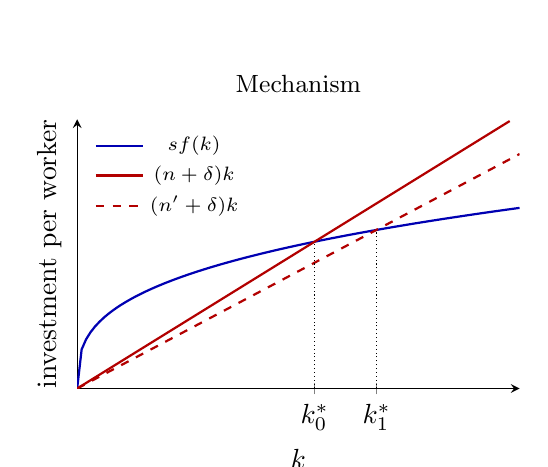
\begin{tikzpicture}
\begin{axis}[width=7.2cm,height=5cm,axis lines=left,xmin=0,xmax=9,ymin=0,ymax=0.62,
  xlabel={$k$},ylabel={investment per worker},xtick={4.83,6.09},xticklabels={$k^\ast_0$,$k^\ast_1$},
  ytick=\empty,title={\small Mechanism},legend style={font=\scriptsize,at={(0.02,0.98)},anchor=north west,draw=none}]
\addplot[thick,blue!70!black,domain=0:9,samples=100]{0.2*x^(1/3)};
\addplot[thick,red!70!black,domain=0:8.8]{0.07*x};
\addplot[thick,red!70!black,dashed,domain=0:9]{0.06*x};
\legend{$sf(k)$,$(n+\delta)k$,$(n'+\delta)k$}
\draw[densely dotted] (axis cs:4.83,0)--(axis cs:4.83,0.338);
\draw[densely dotted] (axis cs:6.09,0)--(axis cs:6.09,0.365);
\end{axis}
\end{tikzpicture}\quad
\begin{tikzpicture}
\begin{axis}[width=7.2cm,height=5cm,axis lines=left,xmin=-10,xmax=60,ymin=0.5,ymax=0.63,
  xlabel={time},ylabel={$\ln y$},xtick={0},xticklabels={$t_0$},ytick={0.525,0.602},
  yticklabels={$\ln y^\ast_0$,$\ln y^\ast_1$},title={\small Time path}]
\addplot[thick,blue!70!black,domain=-10:0]{0.5249};
\addplot[thick,blue!70!black,domain=0:60,samples=60]{0.6019-(0.6019-0.5249)*exp(-0.04*x)};
\addplot[densely dotted,domain=-10:60]{0.6019};
\end{axis}
\end{tikzpicture}
\end{center}
{\footnotesize Left: $n$ falls, the break-even ray rotates down, $k^\ast$ rises. Right: $\ln y$ rises
during the transition and flattens; $\ln Y$ (not drawn) has slope $n=2\%$ before and $n'=1\%$ after.}
\refbib{Kurlat ch.~4, \S4.2 (comparative statics), pp.~59--61.}
\end{sol}

\medskip
\textbf{b)} (3 points) Same model with $\alpha=0.35$ and $n+\delta=0.07$; Brazil saves 17\% of GDP.
Which statement is correct about the golden-rule saving rate and the effect on steady-state
consumption per worker of raising $s$ from 0.17 to 0.25?
\begin{alternativas}
\item $s_{GR}=0.65$; raising $s$ from 0.17 to 0.25 lowers steady-state consumption per worker.
\item $s_{GR}=0.35$; raising $s$ from 0.17 to 0.25 raises steady-state consumption per worker.
\item $s_{GR}=0.35$; raising $s$ from 0.17 to 0.25 lowers steady-state consumption per worker.
\item $s_{GR}=1.00$; raising $s$ from 0.17 to 0.25 raises steady-state consumption per worker.
\end{alternativas}
\gabarito{B.}
\begin{sol}
$c^\ast=f(k^\ast)-(n+\delta)k^\ast$ is maximised at $f'(k_{GR})=n+\delta$; with Cobb--Douglas
$\alpha k^{\alpha-1}=n+\delta$ and $s\,k^{\alpha-1}=n+\delta$ give $\boxed{s_{GR}=\alpha=0.35}$.
$c^\ast(s)=(1-s)\left(\frac{s}{0.07}\right)^{0.35/0.65}$: $c^\ast(0.17)=1.338<c^\ast(0.25)=1.488$.
Below the golden rule a higher $s$ raises long-run consumption (after an initial fall). A uses
$1-\alpha$; C reads only the $(1-s)$ factor; D maximises $k^\ast$, not $c^\ast$.
\refbib{Kurlat ch.~4, \S4.3 (golden rule), pp.~61--63.}
\end{sol}

\medskip
\textbf{c)} (2 points, T or F) Of two economies with the same technology, depreciation and population
growth, the one with lower capital per worker necessarily grows faster.
\gabarito{F.}
\begin{sol}
Convergence is \emph{conditional}: $g_k=s\,k^{\alpha-1}-(n+\delta)$ depends on the distance to each
economy's own steady state, which depends on $s$. With $\alpha=1/3$, $n+\delta=0.07$: $X$ with $k=3$,
$s=0.10$ has $g_k=-2.2\%$; $Z$ with $k=5$, $s=0.30$ has $g_k=+3.3\%$.
\refbib{Kurlat ch.~5, \S5.1--\S5.3 (convergence), pp.~75--86.}
\end{sol}

\medskip
\textbf{d)} (2 points, T or F) If a country's national accounts show a capital share of income of one
third, the same as in undistorted economies with $\alpha=1/3$, then its measured TFP reflects only
technology.
\gabarito{F.}
\begin{sol}
Normal factor shares do not rule out distortions. A requirement to hold unproductive capital recorded
as capital leaves $rK/Y=\alpha$ exactly and puts the whole distortion in the residual,
$\hat A=A(1+\theta)^{-\alpha}$ (Question 4).
\refbib{Kurlat ch.~5, \S5.4--\S5.5 (growth and development accounting), pp.~86--95.}
\gap{Lista 1, 4(b): a Solow comparative static in $n$ left blank; Lista 1, 4(a): aggregate vs per
capita (item a). Item (d) previews Lista 2, 2(c).}
\end{sol}

% -----------------------------------------------------------------------------
\questao{(15 points) ``Custo Brasil'' in the growth accounts.
Output is $Y=AK_P^{\alpha}L^{1-\alpha}$ with $\alpha=0.4$, where $K_P$ is productive capital.
Regulation, legal uncertainty and crime force every firm to hold $\theta$ units of \emph{compliance
capital} (duplicate tax-filing systems, armoured vehicles, walls, back-up generators) for each unit of
productive capital. Compliance capital produces nothing, but the national accounts record it as capital
like any other, so measured capital is $K=K_P+\theta K_P$. Capital is rented at $r$ and labour hired
at $w$ in competitive markets. Today $\theta=0.6$.}

\textbf{a)} (5 points) Write aggregate output as a function of $A,K,L,\theta$. What share of measured
capital is unproductive? How much output is lost relative to an economy with $\theta=0$ and the same
$A,K,L$? State the base of your percentage.
\resolespaco
\begin{sol}
\passo{1 --- composition}{$K=(1+\theta)K_P\Rightarrow K_P=K/(1+\theta)$.}
\passo{2 --- output}{$Y=A\left(\dfrac{K}{1+\theta}\right)^{\alpha}L^{1-\alpha}
\;\Rightarrow\;\boxed{Y=\underbrace{A(1+\theta)^{-\alpha}}_{\text{wedge on TFP}}K^{\alpha}L^{1-\alpha}}$.}
\passo{3 --- unproductive share}{$\dfrac{\theta K_P}{(1+\theta)K_P}=\dfrac{0.6}{1.6}=\boxed{37.5\%}$.}
\passo{4 --- output lost}{$\dfrac{Y(\theta)}{Y(0)}=(1.6)^{-0.4}=e^{-0.4\ln1.6}=e^{-0.4\cdot0.4700}=e^{-0.1880}=0.8286$.
\boxed{\text{Output is }17.1\%\text{ below the undistorted level}} (base: $Y(0)$). Equivalently,
removing $\theta$ would raise output by $1/0.8286-1=\boxed{20.7\%}$ (base: $Y(\theta)$).
\#~Careful with the chosen base.}
\intuicao{A third of the capital stock does no work, but output falls by less than a third because
capital has diminishing returns and a share of only 0.4.}
\refbib{Kurlat ch.~5, \S5.4--\S5.5, pp.~86--95.}
\rubrica{
\item $K_P=K/(1+\theta)$ and the boxed $Y$ with the wedge named: 2 pts.
\item Share 37.5\%: 1 pt.
\item Loss 17.1\% (or gain 20.7\%) with the base stated: 2 pts; no base stated: $-1$ pt.
\item Loss computed as $\theta/(1+\theta)=37.5\%$ of output: max.\ 2 pts on the item.
}
\end{sol}

\textbf{b)} (5 points) Write the representative firm's problem and first-order conditions and derive
the measured factor shares $rK/Y$ and $wL/Y$. A development accountant has data on $Y$, $K$, $L$ and
factor payments only. What does she conclude about $\alpha$ and about TFP? Who bears the cost of
$\theta$?
\resolespaco
\begin{sol}
\passo{1 --- problem}{To use $K_P$ productive units the firm must rent $(1+\theta)K_P$:
$\max_{K_P,L}\;AK_P^{\alpha}L^{1-\alpha}-r(1+\theta)K_P-wL$.}
\passo{2 --- FOCs}{$\alpha\dfrac{Y}{K_P}=r(1+\theta)$ and $(1-\alpha)\dfrac{Y}{L}=w$.}
\passo{3 --- shares}{Using $(1+\theta)K_P=K$: $r=\dfrac{\alpha Y}{(1+\theta)K_P}=\alpha\dfrac{Y}{K}$, so
$\boxed{rK/Y=\alpha=0.4}$ and $\boxed{wL/Y=1-\alpha=0.6}$: \emph{undistorted}.}
\passo{4 --- the accountant}{She sets $\hat\alpha=rK/Y=0.4=\alpha$ (correct) and computes
$\hat A=\dfrac{Y}{K^{\hat\alpha}L^{1-\hat\alpha}}=\boxed{A(1+\theta)^{-\alpha}=0.83A}$.
She concludes that Brazil has 17\% lower \emph{technology}. Wrong: technology is $A$; the gap is a
wasted-capital distortion that the data classify as productivity.}
\passo{5 --- incidence}{The rental rate $r=\alpha Y/K$ and the wage
$w=(1-\alpha)\hat A(K/L)^{\alpha}$ are both lower at given $K/L$ by the factor $(1+\theta)^{-\alpha}$.
\#~Workers are also affected: capital and labour are complements.}
\intuicao{Each productive machine drags $\theta$ idle ones with it, so capital looks less productive
by exactly the amount it is paid less: the share is untouched, the level is not.}
\refbib{Kurlat ch.~5, \S5.4 (factor shares and TFP), pp.~86--92.}
\rubrica{
\item Problem with cost $r(1+\theta)K_P$ and both FOCs: 1.5 pts.
\item $rK/Y=\alpha$, $wL/Y=1-\alpha$: 1.5 pts.
\item $\hat\alpha=\alpha$ and $\hat A=A(1+\theta)^{-\alpha}$, read as distortion, not technology: 1.5 pts.
\item Workers also bear the cost: 0.5 pt.
\item Claiming the capital share is distorted ($\hat\alpha\neq\alpha$): max.\ 2 pts on the item.
}
\end{sol}

\textbf{c)} (5 points) A reform (tax simplification, digital filing, lower crime) cuts $\theta$ from
0.6 to 0.28 gradually over the decade 2027--2036, while true $A$ stays constant; $K$ and $L$ grow at
whatever rates they grow. Write the growth-accounting decomposition, compute the average annual Solow
residual, say what it would show if $\theta$ instead \emph{rose} from 0.28 to 0.6, and explain why
this is consistent with Kurlat's reading of the residual.
\resolespaco
\begin{sol}
\passo{1 --- decomposition}{From $Y_t=A(1+\theta_t)^{-\alpha}K_t^{\alpha}L_t^{1-\alpha}$, in logs over the decade:
$\Delta\ln Y=\alpha\,\Delta\ln K+(1-\alpha)\Delta\ln L+\underbrace{\Delta\ln A}_{=0}\underbrace{-\alpha\,\Delta\ln(1+\theta)}_{\Delta\theta}$.
The accountant computes $\text{residual}=\Delta\ln Y-\alpha\Delta\ln K-(1-\alpha)\Delta\ln L=\underbrace{g_{\text{TFP}}+\Delta\theta\text{ term}}_{\text{Solow residual}}$.}
\passo{2 --- number}{$\alpha\ln\dfrac{1+\theta}{1+\theta'}=0.4\ln\dfrac{1.6}{1.28}=0.4\ln1.25=0.4\cdot0.2231=0.0893$
over ten years, i.e.\ $\boxed{\approx0.89\text{ pp per year}}$ of measured ``TFP growth'' with zero
technical progress. $\ln\hat A$ goes from $-0.188$ to $-0.099$.}
\passo{3 --- the reverse}{If $\theta$ rose from 0.28 to 0.6 the residual would be
$\boxed{-0.89\text{ pp per year}}$: measured technological regress with unchanged technology.}
\passo{4 --- check}{$K$ and $L$ are subtracted with the right weights (shares are undistorted, (b)),
so the $\theta$ effect lands entirely in the residual whatever $K$ and $L$ do.}
\passo{5 --- Kurlat's reading}{The residual is whatever output growth the measured inputs do not
explain --- ``a measure of our ignorance''. It contains technology \emph{and} the efficiency with which
measured inputs are used (regulation, institutions, misallocation). A falling $\theta$ is exactly an
efficiency gain in the use of measured capital, so it belongs in the residual.}
\begin{center}
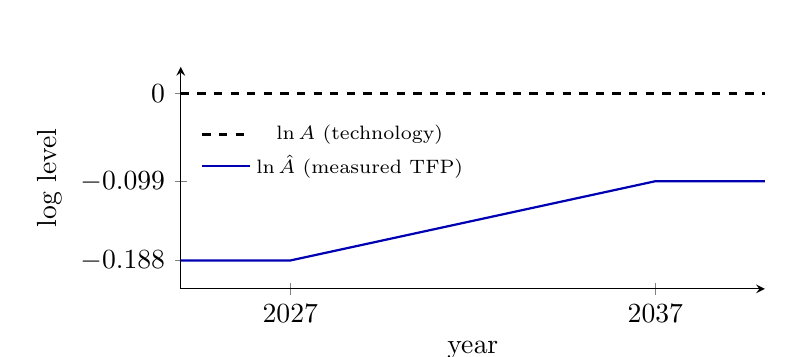
\begin{tikzpicture}
\begin{axis}[width=9cm,height=4.4cm,axis lines=left,xmin=2024,xmax=2040,ymin=-0.22,ymax=0.03,
  xlabel={year},ylabel={log level},xtick={2027,2037},xticklabels={2027,2037},
  ytick={-0.188,-0.099,0},yticklabels={$-0.188$,$-0.099$,$0$},
  legend style={font=\scriptsize,at={(0.02,0.62)},anchor=west,draw=none},
  x tick label style={/pgf/number format/1000 sep=}]
\addplot[thick,dashed,black,domain=2024:2040]{0};
\addplot[thick,blue!70!black] coordinates {(2024,-0.188) (2027,-0.188) (2037,-0.0987) (2040,-0.0987)};
\legend{$\ln A$ (technology),$\ln\hat A$ (measured TFP)}
\end{axis}
\end{tikzpicture}\\
{\footnotesize Measured TFP rises 0.89 pp a year during the reform and stops when $\theta$ stops falling; true $A$ never moves.}
\end{center}
\intuicao{The reform does not invent anything; it releases capital that was already paid for. The
data see more output from the same measured inputs and call it productivity.}
\refbib{Kurlat ch.~5, \S5.4--\S5.5 (growth accounting and what the residual contains), pp.~86--95.}
\rubrica{
\item Decomposition with the residual split into $g_{\text{TFP}}$ and the $\theta$ term: 1.5 pts.
\item $0.4\ln1.25=0.089$, about 0.89 pp per year: 1.5 pts (arithmetic slip: $-1$ pt).
\item Reverse case with the sign: 1 pt.
\item Kurlat's reading of the residual: 1 pt.
\item Residual set to zero ``because $A$ is constant'': max.\ 1 pt on the item.
}
\gap{Lista 2, 2(d), left blank: the growth-accounting residual when a capital-wasting distortion
falls. Items (a)--(c) of Lista 2 were right; this question re-asks (d) with new numbers.}
\end{sol}

% =============================================================================
\bloco{III}{Microfoundations: consumption, labour and general equilibrium}{Lectures 4--6 \,\textbullet\, 25 points}

\questao{(10 points) Objective items.}

\textbf{a)} (3 points) A two-period household (Kurlat ch.~6) has $u=\ln c_1+\beta\ln c_2$ with
$\beta=1$, faces $r=0$, can borrow and lend freely and earns $y_1=y_2=10{,}000$ reais. Consider three
separate scenarios, each against this baseline: (i) a one-off bonus of 1{,}000 today (an extraordinary
FGTS withdrawal); (ii) a credible announcement today of a raise of 1{,}000 paid in period 2 only;
(iii) a permanent raise of 1{,}000 in both periods. The changes in $c_1$ in (i), (ii), (iii) are:
\begin{alternativas}
\item 1{,}000; \ 0; \ 1{,}000
\item 500; \ 0; \ 1{,}000
\item 500; \ 500; \ 1{,}000
\item 500; \ 500; \ 500
\item 1{,}000; \ 500; \ 2{,}000
\end{alternativas}
\gabarito{C.}
\begin{sol}
With log utility $c_1=\dfrac{y_1+y_2/(1+r)}{1+\beta}=\dfrac{y_1+y_2}{2}$. (i) $\Delta W=1{,}000\Rightarrow\Delta c_1=500$;
(ii) $\Delta W=1{,}000/(1+0)=1{,}000\Rightarrow\Delta c_1=500$: news about future income moves
consumption \emph{today}, financed by borrowing; (iii) $\Delta W=2{,}000\Rightarrow\Delta c_1=1{,}000$.
\boxed{500;\ 500;\ 1{,}000}. A is Keynesian (current income only); B ignores the news.
\refbib{Kurlat ch.~6, \S6.2--\S6.3 (permanent income), pp.~105--120.}
\end{sol}

\medskip
\textbf{b)} (3 points) The government must raise a given revenue from households that save. It can tax
interest income or levy a lump-sum tax in period 2 that raises the same revenue. With CRRA utility,
which statement is correct?
\begin{alternativas}
\item Only the tax on interest changes $c_2/c_1$, through the net return in the Euler equation; at equal revenue the lump sum gives higher utility.
\item Both taxes lower $c_2/c_1$ by the same amount, because they raise the same revenue in present value and so lower wealth equally.
\item Only the lump-sum tax changes $c_2/c_1$, because it lowers wealth; the tax on interest is neutral once its revenue is fixed.
\item Only the tax on interest changes $c_2/c_1$, through the net return in the Euler equation; at equal revenue both give the same utility.
\end{alternativas}
\gabarito{A.}
\begin{sol}
Euler: $u'(c_1)=\beta[1+r(1-\tau)]u'(c_2)\Rightarrow c_2/c_1=\{\beta[1+r(1-\tau)]\}^{1/\sigma}$: the
\emph{intertemporal margin} is distorted. The lump sum shifts the budget line in parallel and leaves
$c_2/c_1=[\beta(1+r)]^{1/\sigma}$. At equal revenue $T=\tau ra$, the plan chosen under the interest tax
costs exactly $y_1+(y_2-T)/(1+r)$ at market prices, so it was affordable under the lump sum and not
chosen: \boxed{U^{\text{lump sum}}>U^{\text{interest tax}}}, the difference being deadweight loss
(D misses this).
\refbib{Kurlat ch.~6, \S6.2--\S6.4 (taxes in the two-period model), pp.~105--126.}
\end{sol}

\medskip
\textbf{c)} (2 points, T or F) A household with $u=\ln c_1+\beta\ln c_2$ earns $y_1>0$ in period 1 and
nothing in period 2 (no taxes), so it is a net saver. When $r$ rises it raises $c_1$, because for a
saver the income effect of a higher return dominates the substitution effect.
\gabarito{F.}
\begin{sol}
$c_1=\dfrac{y_1}{1+\beta}$, independent of $r$: with $\sigma=1$ and no future income to revalue, the
income and substitution effects cancel \emph{exactly}. The sign of $\partial c_1/\partial r$ is that
of $\sigma-1$; the income effect wins only if $\sigma>1$.
\refbib{Kurlat ch.~6, \S6.2 (the effect of interest rates), pp.~108--115.}
\end{sol}

\medskip
\textbf{d)} (2 points, T or F) With $u=\ln c-\chi\,h^{1+\eta}/(1+\eta)$ and no non-labour income, hours
do not respond to a permanent change in the wage (the Marshallian elasticity is zero). Therefore a
temporary, anticipated wage rise within a life of given wealth leaves hours unchanged too: the Frisch
elasticity is also zero.
\gabarito{F.}
\begin{sol}
Marshallian: $\chi h^{\eta}=w/c=w/(wh)=1/h$, hours constant. Frisch (marginal utility of wealth
$\mu$ fixed): $\chi h^{\eta}=\mu w\Rightarrow\varepsilon^F=1/\eta>0$. The ordering is
$\varepsilon^F\ge\varepsilon^H\ge\varepsilon^M$; a zero Marshallian elasticity means two effects
cancel, not that labour supply is unresponsive.
\refbib{Kurlat ch.~7, \S7.3--\S7.4, pp.~137--142.}
\gap{Lista 3, 1(b): no permanent-income story for a rise in expected $y_2$ (item a). Lista 3, 2(d): the
equal-revenue lump-sum comparison and the distorted margin were never stated (item b).}
\end{sol}

% -----------------------------------------------------------------------------
\questao{(15 points) An agribusiness productivity boom in general equilibrium.
A one-period economy has a fixed capital stock $\bar K$. The representative household owns $\bar K$ and
the firm, has one unit of time and utility $u=\dfrac{c^{1-\sigma}}{1-\sigma}+\psi\ln(1-L)$ with
$\psi=2/3$ ($\sigma$ is the curvature of utility; $1/\sigma$ the elasticity of substitution).
The competitive firm produces $Y=A\bar K^{\alpha}L^{1-\alpha}$ with $\alpha=1/3$. At the baseline
$A\bar K^{\alpha}=2^{2/3}$ and $\sigma=2$. New seed varieties raise $A$ in agriculture, which we treat
as a rise in aggregate $A$.}

\textbf{a)} (5 points) Write the household's and the firm's problems, the first-order conditions and the
market-clearing conditions. Show that profits are zero. Reduce the equilibrium to one equation in $L$,
verify that $L=1/2$ at the baseline, and compute $c$, $w$ and $r^K\bar K$.
\resolespaco
\begin{sol}
\passo{1 --- household}{$\max_{c,L}\ \frac{c^{1-\sigma}}{1-\sigma}+\psi\ln(1-L)$ s.t.\
$c=wL+r^K\bar K+\Pi$. FOC: $\boxed{\dfrac{\psi}{1-L}=w\,c^{-\sigma}}$ (MRS between leisure and
consumption $=$ real wage).}
\passo{2 --- firm}{$\max_L\ A\bar K^{\alpha}L^{1-\alpha}-wL-r^K\bar K$:
$w=(1-\alpha)\dfrac{Y}{L}$ (MPL), $r^K=\alpha\dfrac{Y}{\bar K}$ (MPK).
$\Pi=Y-(1-\alpha)Y-\alpha Y=0$ (constant returns, Euler's theorem).}
\passo{3 --- clearing}{Goods: $c=Y$ (no investment, no government). Capital: supply fixed at $\bar K$.}
\passo{4 --- one equation}{Let $\tilde A=A\bar K^{\alpha}$, so $c=\tilde AL^{1-\alpha}$ and
$w=(1-\alpha)\tilde AL^{-\alpha}$. Substituting into Step 1:
$\boxed{\psi\dfrac{L^{\alpha+(1-\alpha)\sigma}}{1-L}=(1-\alpha)\tilde A^{1-\sigma}}$ (MRS $=$ MPL).
The left side rises in $L$, so the solution is unique.}
\passo{5 --- verify}{$\sigma=2$: exponent $\tfrac13+\tfrac43=\tfrac53$. LHS at $L=\tfrac12$:
$\tfrac23\cdot\dfrac{2^{-5/3}}{2^{-1}}=\tfrac23\,2^{-2/3}$. RHS: $\tfrac23(2^{2/3})^{-1}=\tfrac23\,2^{-2/3}$ \checkmark.
Then $\boxed{c=Y=2^{2/3}\,2^{-2/3}=1}$, $\boxed{w=\tfrac23\cdot1/\tfrac12=\tfrac43}$,
$\boxed{r^K\bar K=\tfrac13}$; check $wL+r^K\bar K=\tfrac23+\tfrac13=1=Y$.}
\refbib{Kurlat ch.~9, \S9.1--\S9.2 (competitive equilibrium), pp.~165--180; ch.~7, \S7.2.}
\rubrica{
\item Both problems and FOCs, including MRS $=w$: 2 pts.
\item Zero profits and $c=Y$: 1 pt.
\item Equation in $L$ and the baseline check with $c,w,r^K\bar K$: 2 pts.
\item Adding the principal $\bar K$ to household income: $-1$ pt (budget no longer matches $c=Y$).
}
\end{sol}

\textbf{b)} (5 points) Derive $d\ln L/d\ln A$ in general and sign it by $\sigma$. Evaluate it at the
baseline and give the first-order effects of a 10\% rise in $A$ on $L$, $w$, $r^K$ and $c$. Explain in
words that match the sign.
\resolespaco
\begin{sol}
\passo{1 --- differentiate}{Log of the equation in (a):
$\ln\psi+[\alpha+(1-\alpha)\sigma]\ln L-\ln(1-L)=\ln(1-\alpha)+(1-\sigma)\ln\tilde A$.
Differentiating, with $d\ln\tilde A=d\ln A$:
$\boxed{\dfrac{d\ln L}{d\ln A}=\dfrac{1-\sigma}{\alpha+(1-\alpha)\sigma+\frac{L}{1-L}}}$.}
\passo{2 --- sign}{The denominator is positive, so the sign is that of $1-\sigma$:
$\sigma<1\Rightarrow L\uparrow$; $\sigma=1\Rightarrow L$ unchanged; $\sigma>1\Rightarrow L\downarrow$.}
\passo{3 --- baseline}{$\sigma=2$, $L=\tfrac12$: $\dfrac{-1}{\frac13+\frac43+1}=\dfrac{-1}{8/3}=\boxed{-0.375}$.}
\passo{4 --- 10\% boom}{$d\ln L=-3.75\%$. $d\ln w=d\ln A-\alpha\,d\ln L=10+\tfrac13(3.75)=\boxed{+11.25\%}$.
$d\ln r^K=d\ln A+(1-\alpha)d\ln L=10-\tfrac23(3.75)=\boxed{+7.5\%}$.
$d\ln c=d\ln Y=d\ln A+(1-\alpha)d\ln L=\boxed{+7.5\%}$.}
\passo{5 --- words}{$A\uparrow\rightarrow w\uparrow$: leisure is dearer (substitution effect, work more)
but the household is richer (income effect, enjoy more leisure). With $\sigma=2$ marginal utility of
consumption falls fast as $c$ rises, so the \emph{income effect dominates} and hours fall. Output and
consumption still rise, by less than $A$.}
\intuicao{$\sigma$ measures how fast extra consumption loses value. Above one, a richer household
prefers to take part of its gain as leisure; at exactly one the two effects cancel.}
\refbib{Kurlat ch.~7, \S7.2 (income and substitution effects), pp.~131--137; ch.~9, \S9.2.}
\rubrica{
\item Correct derivative: 2 pts. Sign by $\sigma$ with the three cases: 1 pt.
\item $-0.375$ and the four effects: 1 pt (arithmetic slip: $-1$ pt, non-cumulative).
\item Words matching the sign: 1 pt.
\item Words describing only the substitution effect (``higher wage, so they work more'') when the derivative is negative: max.\ 3 pts on the item.
}
\end{sol}

\textbf{c)} (5 points) Now set $\sigma=1$. The government taxes labour income at $\tau=0.25$.
Compute equilibrium hours without the tax and in two cases: (i) the revenue is rebated lump sum;
(ii) the revenue is thrown away (spent on something with no value to the household). Explain why hours
fall in (i) even with log utility, why they fall less in (ii), and what happens in (ii) if $\alpha\to0$.
\resolespaco
\begin{sol}
\passo{1 --- FOC with the tax}{Budget $c=(1-\tau)wL+r^K\bar K+T$; FOC
$\dfrac{\psi}{1-L}=\dfrac{(1-\tau)w}{c}$, with $w=(1-\alpha)Y/L$.}
\passo{2 --- no tax}{$c=Y$: $\psi\dfrac{L}{1-L}=1-\alpha\Rightarrow\tfrac23\dfrac{L}{1-L}=\tfrac23\Rightarrow\boxed{L=\tfrac12}$.}
\passo{3 --- (i) rebate}{$T=\tau wL\Rightarrow c=Y$:
$\psi\dfrac{L}{1-L}=(1-\tau)(1-\alpha)=0.75\cdot\tfrac23=0.5\Rightarrow
L=\dfrac{0.5}{\frac23+0.5}=\boxed{\tfrac37\approx0.429}$.}
\passo{4 --- (ii) thrown away}{$c=Y-\tau wL=Y[1-\tau(1-\alpha)]$:
$\psi\dfrac{L}{1-L}=\dfrac{(1-\tau)(1-\alpha)}{1-\tau(1-\alpha)}=\dfrac{0.5}{5/6}=0.6\Rightarrow
\dfrac{L}{1-L}=0.9\Rightarrow\boxed{L=\tfrac{9}{19}\approx0.474}$.}
\passo{5 --- why (i) falls}{The rebate hands back the revenue: total income is unchanged ($c=Y$) but the
price of leisure falls to $(1-\tau)w$. The transfer is non-labour income that does not shrink with
the net wage, so the tax acts as a \emph{compensated} wage cut: a pure substitution effect $\Rightarrow$
hours fall, with log utility or not.}
\passo{6 --- why (ii) falls less, and $\alpha\to0$}{Without the rebate the household is poorer. On
labour income, log utility makes the income and substitution effects cancel; only the capital rents
$r^K\bar K$ (share $\alpha$), unearned income that does not fall with the net wage, leave a residual
effect. As $\alpha\to0$ the right side tends to $(1-\tau)/(1-\tau)=1$ and
\boxed{L\text{ is independent of }\tau}.}
\intuicao{With log consumption utility, a wage tax changes hours only through non-labour income ---
the transfer and the capital rents. Set that income to zero and the effect vanishes; the story must
therefore be about the transfer.}
\refbib{Kurlat ch.~7, \S7.2 (taxes and labour supply), pp.~131--137; ch.~9, \S9.2.}
\rubrica{
\item FOC with $(1-\tau)w$: 1 pt. $L=\tfrac12$, $\tfrac37$, $\tfrac{9}{19}$: 2 pts (slip: $-1$ pt).
\item Rebate $=$ compensated change, substitution effect only: 1 pt.
\item Role of non-labour income in (ii) and the $\alpha\to0$ limit: 1 pt.
\item Explaining (i) by ``the tax lowers the wage, so leisure is cheaper'' with no role for the transfer, and claiming the same in (ii): max.\ 2 pts on the item.
}
\gap{Lista 4, 1(b): with log utility labour responds to a wage tax only through the transfer, but the
words described the substitution effect. Lista 5, Q1: the sign of $d\ln L/d\ln A$ is that of
$1-\sigma$ and the words must match it.}
\end{sol}

% =============================================================================
\bloco{IV}{Money, inflation and the New-Keynesian AS--AD model}{Lectures 7--9 \,\textbullet\, 25 points}

\questao{(10 points) Objective items.}

\textbf{a)} (3 points) A flexible-price economy (Kurlat ch.~11) has real money demand $M/P=Y\,\ell(i)$,
$\ell'<0$, with $Y$ and $r$ fixed by the real side. Which statement is correct?
\begin{alternativas}
\item A one-off 10\% rise in $M$ raises $P$ by 10\% and leaves $Y$, $r$ and $M/P$ unchanged; a permanent rise in money growth also leaves $M/P$ unchanged, as money is superneutral.
\item A one-off 10\% rise in $M$ raises $P$ by 10\% and leaves $Y$, $r$ and $M/P$ unchanged; a permanent rise in money growth raises $i$ and lowers $M/P$.
\item A one-off 10\% rise in $M$ lowers $i$ through a liquidity effect and raises $Y$ for good; a permanent rise in money growth raises $i$ and lowers $M/P$.
\item A one-off 10\% rise in $M$ raises $P$ by 10\% and leaves $Y$, $r$ and $M/P$ unchanged; under a Selic target the Copom fixes both $i$ and $M$ independently.
\end{alternativas}
\gabarito{B.}
\begin{sol}
Level change: neutrality, $P$ moves one for one. Growth change: $\pi\uparrow\Rightarrow i=r+\pi\uparrow
\Rightarrow\ell(i)\downarrow$: money is neutral but \emph{not superneutral} (A). C is IS--LM with
flexible prices. D: with $i$ as the instrument, $M=P\,Y\ell(\bar\imath)$ is \emph{determined} by the
money market; the bank cannot also choose $M$.
\refbib{Kurlat ch.~11, \S11.1--\S11.2, pp.~205--215; ch.~10 on the instrument.}
\end{sol}

\medskip
\textbf{b)} (3 points) Real money demand is $M/P=0.10\,Y\,e^{-4\pi}$ (Cagan form, $\pi$ in decimal per
year), $Y$ is constant and in steady state $\pi$ equals money growth. The inflation rate that maximises
seigniorage, and seigniorage at that rate, are:
\begin{alternativas}
\item $\pi=12.5\%$; seigniorage $0.76\%$ of GDP
\item $\pi=25\%$; seigniorage $2.50\%$ of GDP
\item $\pi=50\%$; seigniorage $0.68\%$ of GDP
\item $\pi=25\%$; seigniorage $0.92\%$ of GDP
\end{alternativas}
\gabarito{D.}
\begin{sol}
$S/Y=\pi\cdot0.10e^{-4\pi}$; $\frac{d}{d\pi}=0.10e^{-4\pi}(1-4\pi)=0\Rightarrow\boxed{\pi=1/a=25\%}$;
$S/Y=0.25\cdot0.10\cdot e^{-1}=\boxed{0.92\%}$. B ignores the erosion of the base ($0.25\times0.10$);
A and C are off the peak ($0.76\%$, $0.68\%$).
\refbib{Kurlat ch.~11, \S11.3 (seigniorage) and Exercise 11.6 (Cagan), pp.~215--222.}
\end{sol}

\medskip
\textbf{c)} (2 points, T or F) In Benigno's AS--AD model, a cut in the Selic moves the economy along the
AS curve.
\gabarito{T.}
\begin{sol}
$i$ enters only AD. The cut shifts AD up and to the right; AS (anchored at $(p^e,y_n)$) does not move,
so the new equilibrium lies further up the same AS: $y\uparrow$, $p\uparrow$.
\refbib{Benigno (2015), \S5, Figs.~3--5, pp.~509--511.}
\end{sol}

\medskip
\textbf{d)} (2 points, T or F) In Benigno's model, natural output $y_n$ differs from efficient output
$y_e$ because a fraction of prices is sticky.
\gabarito{F.}
\begin{sol}
$y_n$ is the flexible-price equilibrium, $y_e$ the planner's choice; the stickiness share $\alpha$ is
in neither. The gap is the mark-up wedge (market power and taxes): $y_n-y_e=-\mu/(\sigma^{-1}+\eta)$.
Stickiness explains $y\neq y_n$.
\refbib{Benigno (2015), \S4.2--\S4.4, eqs.~(15), (19), pp.~508--509.}
\gap{Lista 6, 1(c)--(d): flexible prices $\Rightarrow$ neutrality; under an interest-rate instrument
the money market determines $M$ (item a). Lista 7 traps 1 and 4 (items c, d).}
\end{sol}

% -----------------------------------------------------------------------------
\questao{(15 points) A mark-up shock in fuel distribution.
A merger wave concentrates fuel distribution and raises firms' desired mark-up by 4.4\% for one period
only. Use Benigno's model in log deviations from an efficient steady state, with no public spending
($g=0$), no tax changes, $\bar p=p^e=0$ and $\bar y_n=0$:
\[
\text{AS: } p-p^e=\kappa(y-y_n),\quad \kappa=\frac{(1-\alpha)(\sigma^{-1}+\eta)}{\alpha};\qquad
\text{AD: } y=\bar y_n-\sigma\left[i-(\bar p-p)-\rho\right].
\]
Calibration: $\alpha=0.66$ (share of sticky prices), $\sigma=0.5$, $\eta=0.2$, $\theta=8$, $\rho=5\%$.
Before the shock $i=\rho$, $y=y_n=y_e=0$ and $p=p^e$. At first the Copom keeps the Selic at 5\%.}

\textbf{a)} (5 points) Which curve shifts and which does not, and why? Find $y$ and $p$, and the signs
of $y-y_n$ and $y-y_e$. Draw the AS--AD diagram and the time path of $y$ and $p$ over the short run
(period 1) and the long run (period 2).
\resolespaco
\begin{sol}
\passo{1 --- slope}{$\kappa=\dfrac{0.34\cdot(2+0.2)}{0.66}=\dfrac{0.748}{0.66}=1.133$; $\sigma\kappa=0.567$.}
\passo{2 --- what shifts}{$y_n=\dfrac{(1+\eta)a-\mu}{\sigma^{-1}+\eta}\Rightarrow dy_n=-\dfrac{4.4}{2.2}=\boxed{-2\%}$;
$y_e$ has no $\mu$, $dy_e=0$. \boxed{\text{AS shifts up/left}} through $(p^e,y_n'=-2)$, by
$\kappa\cdot2=2.27$ pp at given $y$ ($=\frac{1-\alpha}{\alpha}d\mu=0.515\cdot4.4$ \checkmark).
\boxed{\text{AD does not shift}}: $\mu$ is not in AD, $i$ is unchanged, and a \emph{temporary} shock leaves $\bar y_n$ unchanged.}
\passo{3 --- equilibrium}{AD with $i=\rho$: $p=-y/\sigma=-2y$. AS: $p=1.133(y+2)$.
$-2y=1.133y+2.267\Rightarrow y=-\dfrac{2.267}{3.133}=\boxed{-0.72\%}$, $\boxed{p=+1.45\%}$: stagflation.
(Closed form: $dy=\frac{\sigma\kappa}{1+\sigma\kappa}dy_n$, $dp=-\frac{\kappa}{1+\sigma\kappa}dy_n$.)}
\passo{4 --- two gaps}{$\boxed{y-y_n=-0.72+2=+1.28>0}$ (why prices rise: AS responds to $y-y_n$);
$\boxed{y-y_e=-0.72<0}$ (why welfare falls).}
\passo{5 --- chain}{$\mu\uparrow\rightarrow$ adjusting firms raise prices $\rightarrow p\uparrow
\rightarrow$ real rate $i-(\bar p-p)\uparrow\rightarrow c\downarrow\rightarrow y\downarrow$ along AD.
LR: the shock is over, all firms reset, $y=\bar y_n=0$, $p=\bar p=0$.}
\begin{center}
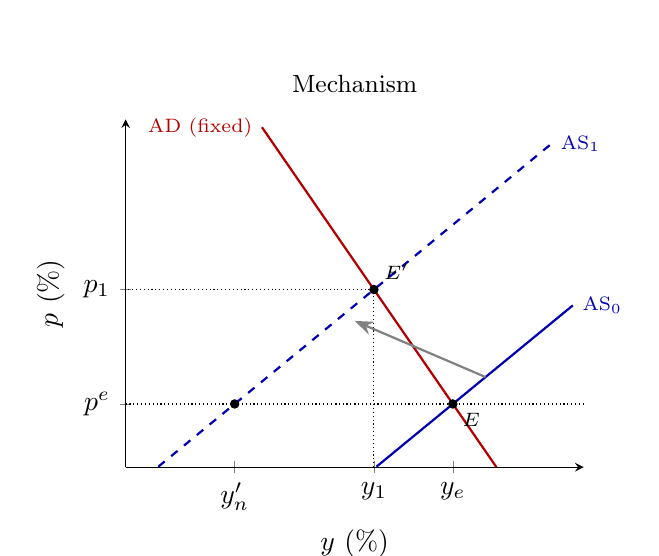
\begin{tikzpicture}
\begin{axis}[width=7.4cm,height=6cm,axis lines=left,xmin=-3,xmax=1.2,ymin=-0.8,ymax=3.6,clip=false,
  xlabel={$y$ (\%)},ylabel={$p$ (\%)},xtick={-2,-0.7234,0},xticklabels={$y_n'$,$y_1$,$y_e$},
  ytick={0,1.4468},yticklabels={$p^e$,$p_1$},title={\small Mechanism}]
\addplot[densely dotted,domain=-3:1.2]{0};
\addplot[thick,blue!70!black,domain=-0.7:1.1]{1.1333*x};
\addplot[thick,blue!70!black,dashed,domain=-2.7:0.9]{1.1333*(x+2)};
\addplot[thick,red!70!black,domain=-1.75:0.4]{-2*x};
\node[font=\scriptsize,blue!70!black,anchor=west] at (axis cs:1.1,1.25) {AS$_0$};
\node[font=\scriptsize,blue!70!black,anchor=west] at (axis cs:0.9,3.29) {AS$_1$};
\node[font=\scriptsize,red!70!black,anchor=east] at (axis cs:-1.75,3.5) {AD (fixed)};
\addplot[only marks,mark=*,mark size=1.5pt] coordinates {(0,0) (-0.7234,1.4468) (-2,0)};
\node[font=\scriptsize,anchor=north west] at (axis cs:0,0) {$E$};
\node[font=\scriptsize,anchor=south west] at (axis cs:-0.72,1.45) {$E'$};
\draw[densely dotted] (axis cs:-0.7234,-0.8)--(axis cs:-0.7234,1.4468)--(axis cs:-3,1.4468);
\draw[-{Stealth},thick,gray] (axis cs:0.3,0.34)--(axis cs:-0.9,1.05);
\end{axis}
\end{tikzpicture}\quad
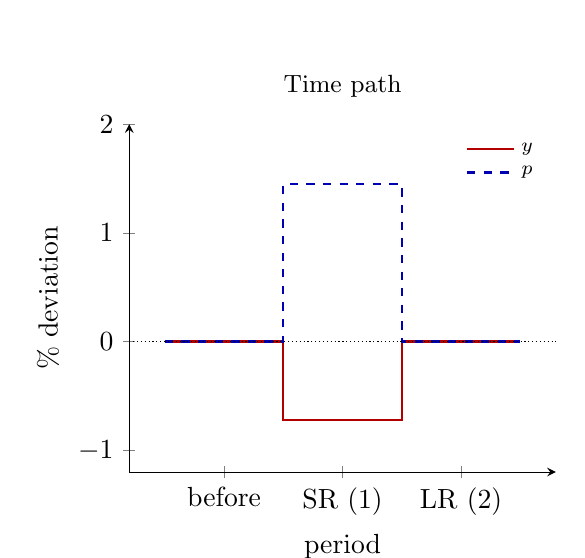
\begin{tikzpicture}
\begin{axis}[width=7cm,height=6cm,axis lines=left,xmin=-0.3,xmax=3.3,ymin=-1.2,ymax=2,
  xlabel={period},xtick={0.5,1.5,2.5},xticklabels={before,SR (1),LR (2)},ylabel={\% deviation},
  title={\small Time path},legend style={font=\scriptsize,draw=none,at={(0.98,0.98)},anchor=north east}]
\addplot[thick,red!70!black,const plot] coordinates {(0,0) (1,-0.7234) (2,0) (3,0)};
\addplot[thick,blue!70!black,dashed,const plot] coordinates {(0,0) (1,1.4468) (2,0) (3,0)};
\addplot[densely dotted,domain=-0.3:3.3]{0};
\legend{$y$,$p$}
\end{axis}
\end{tikzpicture}
\end{center}
\intuicao{The mark-up raises prices at any output; with $\bar p$ anchored, a higher $p$ is a higher real
rate, so demand falls along AD. Output does not fall all the way to $y_n'$ because the sticky firms keep
selling at $p^e$.}
\refbib{Benigno (2015), \S7, Fig.~9, pp.~513--514; \S5, eqs.~(20)--(21).}
\rubrica{
\item AS shifts up/left and AD explicitly does \emph{not} move, with reasons: 1.5 pts.
\item $y=-0.72$, $p=+1.45$: 1 pt (slip: $-1$ pt).
\item Both gaps with opposite signs: 1 pt.
\item Diagram: axes, AS$_0$, AS$_1$ and the unmoved AD labelled, direction of shift: 1 pt; time path SR/LR: 0.5 pt.
\item Shifting AD: max.\ 2 pts on the item. Reporting a single ``output gap'': max.\ 3.5 pts.
}
\end{sol}

\textbf{b)} (5 points) With $u(C)=\dfrac{C^{1-1/\sigma}}{1-1/\sigma}$, $v(L)=\dfrac{L^{1+\eta}}{1+\eta}$,
$Y=AL$ and $C=Y$, the market's labour-supply condition is $\text{MRS}=A/(1+\mu)$ and the planner's is
$\text{MRS}=A$. Derive both, log-linearise, and show $y_n-y_e=-\mu/(\sigma^{-1}+\eta)$. Explain why sticky
prices play no role, and evaluate the gap for this shock.
\resolespaco
\begin{sol}
\passo{1 --- planner}{$\max_Y u(Y)-v(Y/A)$: $u'(Y)=v'(L)/A\Rightarrow\boxed{\dfrac{v'(L)}{u'(C)}=A}$
(MRS $=$ MRT).}
\passo{2 --- market}{Flexible-price firms set $P=(1+\mu)W/A\Rightarrow W/P=A/(1+\mu)$; the household sets
MRS $=W/P$: $\boxed{\dfrac{v'(L)}{u'(C)}=\dfrac{A}{1+\mu}}$. Same condition up to the wedge $1+\mu$.}
\passo{3 --- logs}{$\ln v'=\eta l=\eta(y-a)$; $\ln u'=-\sigma^{-1}c=-\sigma^{-1}y$. So
$\ln\text{MRS}=\eta(y-a)+\sigma^{-1}y$. Planner: $=a\Rightarrow y_e=\dfrac{(1+\eta)a}{\sigma^{-1}+\eta}$.
Market: $=a-\mu\Rightarrow y_n=\dfrac{(1+\eta)a-\mu}{\sigma^{-1}+\eta}$.}
\passo{4 --- subtract}{$\boxed{y_n-y_e=-\dfrac{\mu}{\sigma^{-1}+\eta}}=-\dfrac{4.4}{2.2}=\boxed{-2\%}$.}
\passo{5 --- no stickiness}{$\alpha$ appears in neither condition: $y_n$ is the equilibrium when
\emph{all} prices are flexible; $y_e$ is the planner's, with no prices at all. \#~Stickiness explains
$y\neq y_n$ (it sits in $\kappa$); market power and taxes explain $y_n\neq y_e$. A productivity shock
moves both by $(1+\eta)/(\sigma^{-1}+\eta)$: efficient, no gap.}
\intuicao{A firm with market power pays labour $A/(1+\mu)$ of what it produces; households work until
their MRS equals what they are paid, not what they produce, so the market works and produces too little.}
\refbib{Benigno (2015), \S4.1--\S4.4, eqs.~(14), (15), (19), pp.~507--509.}
\rubrica{
\item Planner MRS $=A$ and market MRS $=A/(1+\mu)$ derived: 2 pts.
\item Log-linearisation and the boxed gap: 1.5 pts; $-2\%$: 0.5 pt.
\item Why stickiness plays no role: 1 pt.
\item Attributing $y_n\neq y_e$ to sticky prices: max.\ 2 pts on the item.
}
\end{sol}

\textbf{c)} (5 points) The Copom minimises $\mathcal L=\phi_y(y-y_e)^2+\phi_p(p-p^e)^2$ with Benigno's
welfare weights $\phi_y=\tfrac12$, $\phi_p=\theta/(2\kappa)$, subject to AS. Derive the targeting rule by
substitution, the optimal $y$ and $p$ and the split of the shock, and the Selic that implements it.
Explain why AS and not AD is the constraint, and what the money market does. Is the optimal response a
rise or a cut relative to doing nothing, and on what does that sign depend?
\resolespaco
\begin{sol}
\passo{1 --- substitute AS}{$\mathcal L(y)=\phi_y y^2+\phi_p\kappa^2(y-y_n)^2$ (with $y_e=0$).
FOC: $\phi_y y+\phi_p\kappa^2(y-y_n)=0$; using $\kappa(y-y_n)=p-p^e$:
$\boxed{\phi_y(y-y_e)+\kappa\phi_p(p-p^e)=0}$; with the welfare weights, $(y-y_e)+\theta(p-p^e)=0$.}
\passo{2 --- optimum}{$\phi_p\kappa^2/\phi_y=\theta\kappa=8\cdot1.133=9.067$.
$y^o=\dfrac{\theta\kappa}{1+\theta\kappa}y_n=0.901\cdot(-2)=\boxed{-1.80\%}$;
$y^o-y_n=\dfrac{2}{1+\theta\kappa}=0.199$; $p^o-p^e=\kappa\cdot0.199=\boxed{+0.23\%}$.
Split: $1/(1+\theta\kappa)=9.9\%$ of the distance $y_e-y_n$ is accepted as output above $y_n$ (hence
prices); $90.1\%$ is absorbed as an output loss. Check: $-1.80+8(0.225)=0$ \checkmark.}
\passo{3 --- the Selic}{Combining AS and AD: $y-y_n=\dfrac{\sigma}{1+\sigma\kappa}(r_n-i)$, with
$r_n=\rho+\sigma^{-1}(\bar y_n-y_n)=5+2\cdot2=9\%$. So
$i^o=9-\dfrac{1.567}{0.5}(0.199)=9-0.623=\boxed{8.38\%}$. Check on AD: $p=5-8.38+2(1.80)=0.23$ \checkmark.
Strict price stability needs $i=r_n=9\%$; strict output stabilisation $i=9-3.133\cdot2=2.73\%$.
Loss: 1.80 at the optimum vs 7.65 with $i=5\%$.}
\passo{4 --- why AS}{One instrument, $i$, which appears only in AD. For any point on AS there is an $i$
that puts AD through it, so AD restricts nothing: it is how the choice is \emph{implemented}. AS is
private pricing behaviour with $p^e$ predetermined, which policy cannot move within the period: it is
the feasible set, like a budget line. The money market has no role in the choice: with $i$ fixed, the
central bank supplies whatever $M=P\,\ell(Y,i)$ is demanded, so it only determines $M$ --- which is why
the model has no LM curve.}
\passo{5 --- sign}{With $i=5\%$, $y-y_n=\dfrac{y_e-y_n}{1+\sigma\kappa}=1.28$; optimum
$\dfrac{y_e-y_n}{1+\theta\kappa}=0.20$. Lower $y-y_n$ needs a higher rate:
\boxed{\text{a rise of }3.38\text{ pp}}. It is a rise iff $\theta\kappa>\sigma\kappa\iff\theta>\sigma$
(general weights: $(\phi_p/\phi_y)\kappa>\sigma$), i.e.\ iff the IT line (slope $-1/\theta$) is flatter
than AD (slope $-1/\sigma$). A dovish bank with $(\phi_p/\phi_y)\kappa<\sigma$ would \emph{cut}.}
\begin{center}
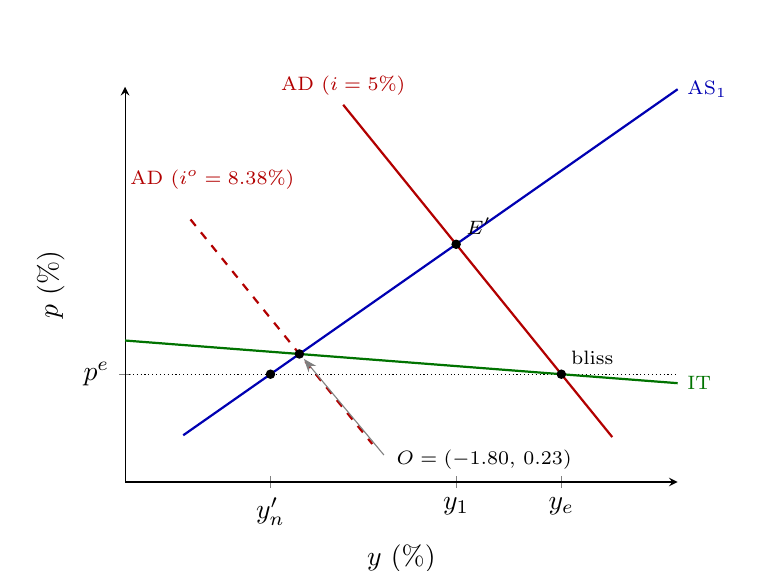
\begin{tikzpicture}
\begin{axis}[width=8.6cm,height=6.6cm,axis lines=left,xmin=-3,xmax=0.8,ymin=-1.2,ymax=3.2,clip=false,
  xlabel={$y$ (\%)},ylabel={$p$ (\%)},xtick={-2,-0.7234,0},xticklabels={$y_n'$,$y_1$,$y_e$},
  ytick={0},yticklabels={$p^e$}]
\addplot[densely dotted,domain=-3:0.8]{0};
\addplot[thick,blue!70!black,domain=-2.6:0.8]{1.1333*(x+2)};
\addplot[thick,green!45!black,domain=-3:0.8]{-x/8};
\addplot[thick,red!70!black,domain=-1.5:0.35]{-2*x};
\addplot[thick,red!70!black,dashed,domain=-2.55:-1.3]{-3.377-2*x};
\node[font=\scriptsize,blue!70!black,anchor=west] at (axis cs:0.8,3.17) {AS$_1$};
\node[font=\scriptsize,green!45!black,anchor=west] at (axis cs:0.8,-0.1) {IT};
\node[font=\scriptsize,red!70!black,anchor=south] at (axis cs:-1.5,3.0) {AD ($i=5\%$)};
\node[font=\scriptsize,red!70!black,anchor=south] at (axis cs:-2.4,1.95) {AD ($i^o=8.38\%$)};
\addplot[only marks,mark=*,mark size=1.5pt] coordinates {(-0.7234,1.4468) (-1.8013,0.2252) (0,0) (-2,0)};
\node[font=\scriptsize,anchor=south west] at (axis cs:-0.72,1.45) {$E'$};
\node[font=\scriptsize,anchor=west] at (axis cs:-1.2,-0.95) {$O=(-1.80,\,0.23)$};
\draw[-{Stealth},gray] (axis cs:-1.22,-0.9)--(axis cs:-1.77,0.17);
\node[font=\scriptsize,anchor=south west] at (axis cs:0,0) {bliss};
\end{axis}
\end{tikzpicture}\\
{\footnotesize The optimum $O$ is where AS$_1$ meets the IT line $(y-y_e)+\theta(p-p^e)=0$; the Copom raises $i$ so that AD shifts
down/left from $E'$ to $O$. AS does not move with policy.}
\end{center}
\intuicao{A mark-up shock moves $y_n$ but not $y_e$, so no rate delivers both targets. Convex losses
make the bank spread the miss; with welfare weights, relative-price dispersion is so costly
($\theta=8$) that it lets only a tenth of the shock into prices.}
\refbib{Benigno (2015), \S11, eqs.~(33)--(35), Fig.~14, pp.~521--523; \S3 on the interest-rate instrument.}
\rubrica{
\item Targeting rule by substitution: 1.5 pts.
\item $y^o=-1.80$, $p^o=+0.23$, split $1/(1+\theta\kappa)$: 1 pt (slip: $-1$ pt).
\item $i^o=8.38\%$ via $r_n=9\%$: 0.5 pt.
\item Why AS is the constraint and the money market determines $M$: 1 pt.
\item Sign relative to no policy with the condition $\theta>\sigma$: 1 pt.
\item Using AD as the constraint: max.\ 2 pts on the item. Targeting $y_n$ instead of $y_e$: max.\ 2.5 pts.
}
\gap{Lista 7 (latest content): a temporary mark-up shock moves only AS; $y-y_n$ vs $y-y_e$; why
$y_n\neq y_e$ (wedge, not stickiness); optimal policy subject to AS and why AD is not a constraint.
Lista 6, 1(d): under a rate instrument the money market determines $M$.}
\end{sol}

\ifsolucoes\else
\vfill
\begin{center}\footnotesize\textit{End of exam.}\end{center}
\fi

\end{document}
"   (run twice)
% Check fonts: pdffonts <file>.pdf  (all Type 1).
% Every number in the key: python simulado_codigo/check_simulado_02.py
% =============================================================================
\documentclass[11pt,a4paper]{article}
\usepackage[utf8]{inputenc}
\usepackage[T1]{fontenc}
\usepackage{lmodern}   % Type 1 vector fonts (replaces PK bitmaps)
\usepackage{cmap}      % ToUnicode CMap -> copyable text and accents
\usepackage[english]{babel}
\usepackage{amsmath,amssymb,amsfonts}
\usepackage[a4paper,margin=2.2cm]{geometry}
\usepackage{enumitem}
\usepackage{fancyhdr}
\usepackage{comment}
\usepackage{xcolor}
\usepackage{microtype}
\usepackage{booktabs}
\usepackage{needspace}
\usepackage{pgfplots}
\pgfplotsset{compat=1.18}
\usetikzlibrary{arrows.meta}

% ====================== CONFIGURATION ======================
\newif\ifsolucoes
\ifdefined\withsolutions\solucoestrue\else\solucoesfalse\fi

\newcommand{\disciplina}{Macroeconomics I --- MPE Insper}
\newcommand{\listatema}{Mock Final Exam 2}
\newcommand{\espacoresol}{6.5cm}

% ====================== MACHINERY ======================
\ifsolucoes\includecomment{sol}\else\excludecomment{sol}\fi

\pagestyle{fancy}\fancyhf{}
\lhead{\footnotesize\disciplina}
\rhead{\footnotesize \listatema\ifsolucoes{} --- Solutions and Rubric\fi}
\cfoot{\footnotesize\thepage}
\renewcommand{\headrulewidth}{0.3pt}
\setlength{\headheight}{14pt}

\setlist{topsep=2pt,itemsep=2pt}
\newcounter{questao}

\newcommand{\bloco}[3]{\Needspace{10\baselineskip}\bigskip\noindent
  {\large\bfseries\color{blue!55!black}Block #1 --- #2}\hfill\textit{(#3)}\par
  \noindent\rule{\linewidth}{0.3pt}\smallskip}
\newcommand{\questao}[1]{\refstepcounter{questao}\medskip\noindent
  \textbf{Question \thequestao.}~#1\par}
\newenvironment{alternativas}{\begin{enumerate}[label=\Alph*.,leftmargin=2.2em,topsep=1pt]}{\end{enumerate}}
\newcommand{\gabarito}[1]{\ifsolucoes\par\noindent\textbf{Answer:}~#1\fi}
\newcommand{\resolespaco}{\ifsolucoes\else\par\textit{Solution:}\vspace{\espacoresol}\par\fi}
\newcommand{\passo}[2]{\par\smallskip\noindent\textbf{Step #1.}~#2}
\newcommand{\intuicao}[1]{\par\smallskip\noindent\textit{Intuition.}~#1}
\newcommand{\refbib}[1]{\par\smallskip\noindent{\footnotesize\color{black!60}\textbf{Ref:} #1}}
\newcommand{\gap}[1]{\par\smallskip\noindent{\footnotesize\color{red!55!black}\textbf{Gap targeted:} #1}}
\newcommand{\trap}[1]{\par\smallskip\noindent{\small\color{red!55!black}\#~#1}}
\newcommand{\rubrica}[1]{\par\smallskip\noindent\textbf{Grading rubric.}\begin{itemize}[leftmargin=1.4em,topsep=1pt]#1\end{itemize}}

% =============================================================================
\begin{document}
\begin{center}
  {\Large\bfseries \disciplina}\\[2pt]
  {\large \listatema\ (Simulado 2) --- 2026, 3rd term}\ifsolucoes\\[2pt]\textit{Solutions and Grading Rubric}\fi
\end{center}
\vspace{2pt}

{\footnotesize\noindent\textbf{Instructions.} Four blocks of 25 points (100 in total). Duration: 3 hours,
closed book, non-programmable calculator allowed. Each block has one objective question (10 points)
and one discursive question (15 points).
\emph{Multiple choice} (items a, b): mark the single correct option; no penalty for a wrong answer.
\emph{True/False} (items c, d): the score of the T/F items is
$\max\{0,\ \text{correct}-\text{wrong}/2\}\times$ item value, i.e.\ every two wrong items cancel one
correct item; blank items do not count as wrong.
\emph{Discursive questions}: show every step; box final answers; sign every derivative before
interpreting it; label axes and curves in diagrams. Notation: Kurlat (2020) in Blocks I--III, Benigno
(2015) in Block IV. All numbers are illustrative.\par}

\ifsolucoes
\medskip
{\footnotesize\noindent\textbf{How the rubric works.} Conceptual caps (``max.\ $x$ pts'') bound an
item whatever else is right. Light penalties ($-1$ pt) apply to arithmetic slips with a correct method.
Caps and penalties are \emph{not cumulative}: when a cap applies, the penalties inside it are ignored.
Each question ends with the graded mistake it retests (``Gap targeted''). Every number below is
recomputed by \texttt{simulado\_codigo/check\_simulado\_02.py}.\par}
\fi

% =============================================================================
\bloco{I}{Measurement and national accounts}{Lecture 1 \,\textbullet\, 25 points}

\questao{(10 points) Objective items.}

\textbf{a)} (3 points) A soy chain in Mato Grosso, one year, values in R\$ million. A fertiliser
producer, which uses no intermediate inputs, sells its whole output, 30, to a soy farm. The farm
harvests soy worth 100: it sells 70 to a crushing plant and exports 30 to China. The crusher sells
soybean oil worth 150 to Brazilian households. By the production (value-added) approach, the chain's
contribution to Brazil's GDP is:
\begin{alternativas}
\item 150
\item 280
\item 180
\item 210
\item 250
\end{alternativas}
\gabarito{C.}
\begin{sol}
Value added $=(30-0)+(100-30)+(150-70)=30+70+80=\boxed{180}$. Check by expenditure:
$C+X=150+30=180$. B (280) is gross production, which counts the intermediate inputs 30 and 70 twice;
A (150) forgets the exports; D (210) subtracts only the soy input; E (250) adds the last two sales.
\refbib{Kurlat ch.~1, \S1.1 (the three approaches), pp.~15--21.}
\end{sol}

\medskip
\textbf{b)} (3 points) IBGE data for a year, in R\$ billion: GDP is 10{,}000; wages earned by
Brazilian residents on short assignments abroad, 50; profits of foreign-owned plants in Brazil sent to
their parent companies, 300; interest on Brazilian bonds held by non-residents, 150; personal transfers
sent home by Brazilians who live permanently abroad, 40. Using Kurlat's definition,
$\text{GNI}=\text{GDP}+F^{\text{out}}-F^{\text{in}}$, where $F^{\text{out}}$ is factor income earned
abroad by residents and $F^{\text{in}}$ factor income earned at home by non-residents, Brazil's GNI is:
\begin{alternativas}
\item 9{,}640
\item 10{,}400
\item 9{,}750
\item 9{,}600
\item 10{,}000
\end{alternativas}
\gabarito{D.}
\begin{sol}
$\text{GNI}=10{,}000+50-300-150=\boxed{9{,}600}$. Profits and interest are \emph{factor} income of
non-residents; the 40 are transfers, not payments to a factor of production, so they are not in GNI
(A adds them). B flips the signs; C leaves the interest out; E confuses territory (GDP) with
ownership (GNI).
\refbib{Kurlat ch.~1, \S1.1, GDP vs GNP.}
\end{sol}

\medskip
\textbf{c)} (2 points, T or F) In a year in which Brazil's gross fixed capital formation equals
17\% of GDP, Brazil's stock of fixed capital rises by 17\% of GDP.
\gabarito{F.}
\begin{sol}
Investment is a gross \emph{flow}; the stock changes by the net flow, $K_{t+1}-K_t=I_t-\delta K_t$.
With, say, $K/Y=3$ and $\delta=4\%$, $\delta K=12\%$ of GDP is replacement, and the stock rises by
only $17-12=5\%$ of GDP.
\refbib{Kurlat ch.~1, eq.~(1.2) and the depreciation discussion, p.~21.}
\end{sol}

\medskip
\textbf{d)} (2 points, T or F) In 2015 Brazil's nominal GDP grew by about 3.8\% while real GDP fell by
about 3.5\%. Hence the GDP deflator rose by less than 3.8\% that year.
\gabarito{F.}
\begin{sol}
$1+\pi_{\text{defl}}=\dfrac{1+g_{\text{nominal}}}{1+g_{\text{real}}}=\dfrac{1.038}{0.965}=1.0756$, so
$\boxed{\pi_{\text{defl}}\approx7.6\%>3.8\%}$. When real output falls, the deflator must grow
\emph{faster} than nominal GDP, not slower.
\refbib{Kurlat ch.~1, \S1.2 (real vs nominal), pp.~22--25.}
\end{sol}
\begin{sol}
\gap{Lista 1, 1(b)--(c): both lost marks were numbers that changed between the line computing them
and the line using them. Items (a) and (d) reward copying each intermediate result exactly.}
\end{sol}

% -----------------------------------------------------------------------------
\questao{(15 points) Brazil and Portugal: exchange rates, prices and welfare.
A think tank compares living standards in Brazil and Portugal with a two-good economy. Per-capita
annual quantities and local prices are:}

\begin{center}\small
\begin{tabular}{@{}lcccc@{}}
\toprule
& \multicolumn{2}{c}{Traded good $T$ (grains, manufactures)} & \multicolumn{2}{c}{Non-traded good $N$ (housing, haircuts, services)}\\
& quantity & price & quantity & price \\
\midrule
Brazil & 5 & 10 reais & 10 & 4 reais \\
Portugal & 10 & 2 euros & 15 & 2 euros \\
\bottomrule
\end{tabular}
\end{center}
\noindent The traded good obeys the law of one price at the market exchange rate. Output per worker is
$A_T=2$, $A_N=5$ in Brazil and $A_T=A_N=5$ in Portugal; within each country labour moves freely between
sectors and firms are competitive.

\textbf{a)} (5 points) Find the market exchange rate (reais per euro), Brazil's GDP per capita in
euros at the market rate and at PPP (Brazil's quantities valued at Portuguese prices), the
Brazil/Portugal ratio under each conversion, the PPP exchange rate and Brazil's price level relative
to Portugal's.
\resolespaco
\begin{sol}
\passo{1 --- market rate}{Law of one price in $T$: 10 reais $=$ 2 euros, so
$\boxed{e=5\text{ reais per euro}}$.}
\passo{2 --- nominal GDP per capita}{Brazil: $5\cdot10+10\cdot4=50+40=90$ reais. Portugal:
$10\cdot2+15\cdot2=20+30=50$ euros.}
\passo{3 --- market-rate conversion}{Brazil $=90/5=18$ euros; ratio $18/50=\boxed{0.36}$.}
\passo{4 --- PPP conversion}{Brazil at Portuguese prices: $5\cdot2+10\cdot2=10+20=30$ euros; ratio
$30/50=\boxed{0.60}$.}
\passo{5 --- PPP rate and price level}{$e^{\text{PPP}}=90/30=\boxed{3\text{ reais per euro}}$.
Relative price level $=e^{\text{PPP}}/e=3/5=\boxed{0.6}$: Brazil's basket costs 60\% of what it costs in
Portugal.}
\passo{6 --- check}{$0.60/0.36=1.667=1/0.6$: the two ratios differ exactly by the price level.}
\refbib{Kurlat ch.~1, \S1.2, international comparisons and PPP, pp.~25--27.}
\rubrica{
\item $e=5$: 1 pt. Market-rate ratio 0.36: 1 pt. PPP ratio 0.60: 1.5 pts. $e^{\text{PPP}}=3$ and price level 0.6: 1.5 pts.
\item Valuing Portugal at Brazilian prices instead is a legitimate PPP (ratio $90/(10\cdot10+15\cdot4)=0.5625$) if stated: full marks for that part; unstated mix of bases: max.\ 3 pts.
\item Arithmetic slip with correct method: $-1$ pt.
}
\end{sol}

\textbf{b)} (5 points) Which good drives the gap between the two ratios? Derive the relative price of
the non-traded good in each country from the firms' and workers' conditions, explain the direction of
the bias of the market-rate comparison (Balassa--Samuelson), and explain why ``transport and trade
costs'' is \emph{not} the explanation here.
\resolespaco
\begin{sol}
\passo{1 --- split Brazil's output by good}{Traded: $50/5=10$ euros at the market rate and
$5\cdot2=10$ euros at PPP --- identical. Non-traded: $40/5=8$ euros at the market rate and
$10\cdot2=20$ euros at PPP. \boxed{\text{The whole 12-euro gap comes from the non-traded good.}}}
\passo{2 --- wage equalisation}{Competitive firms pay the value of the marginal product and workers
move until wages are equal: $W=p_TA_T=p_NA_N\;\Rightarrow\;\boxed{p_N/p_T=A_T/A_N}$.
Brazil: $2/5=0.4=4/10$ \checkmark. Portugal: $5/5=1=2/2$ \checkmark.}
\passo{3 --- mechanism}{$A_T^{BR}/A_T^{PT}=0.4$ while $A_N^{BR}/A_N^{PT}=1$: Brazil's productivity gap
is in traded goods.
$A_T\downarrow\;\rightarrow\;W=p_TA_T\downarrow$ (with $p_T$ tied to the world price)
$\rightarrow\;p_N=W/A_N\downarrow\;\rightarrow$ non-traded goods are cheap in Brazil
$\rightarrow$ the market rate values Brazil's non-traded output at a price nobody pays in Portugal.}
\passo{4 --- direction}{\boxed{\text{The market rate understates Brazil's real output}} (0.36 vs 0.60),
and more so the larger the productivity gap in $T$ relative to $N$. A uniform gap in both sectors
would leave $A_T/A_N$ and hence the price level unchanged.}
\passo{5 --- why not trade costs}{Trade costs are frictions on \emph{traded} goods, and in this
economy the law of one price holds exactly for $T$ --- where the market rate works perfectly (Step 1).
The bias sits in the good that is never traded, for which there is no arbitrage at \emph{any} trade
cost. Trade costs would also push the importer's price up, not produce a systematic ``poorer is
cheaper'' pattern.}
\intuicao{Wages are set by productivity in the sector that faces world prices, and the same wage is
paid to haircutters whose productivity is the same everywhere. Cheap services in poor countries are a
wage fact, not a transport fact.}
\refbib{Kurlat ch.~1, \S1.2, pp.~25--27; Balassa--Samuelson as derived in the course notes
(\texttt{Map/aula-01-mensuracao/04}).}
\rubrica{
\item Decomposition showing the gap is entirely in $N$: 1.5 pts.
\item $p_N/p_T=A_T/A_N$ from wage equalisation, both countries checked: 1.5 pts.
\item Direction (understates) with the mechanism in words: 1 pt.
\item Why trade costs fail: 1 pt.
\item Explaining the gap by trade/import costs: max.\ 2 pts on the item (conceptual cap).
}
\end{sol}

\textbf{c)} (5 points) Welfare beyond GDP. Use Kurlat's consumption-equivalent (Jones--Klenow)
measure with log utility ($\sigma=1$), lognormal consumption within each country and equal leisure
(set the leisure term to zero). A person lives in a country with probability $e=\text{LE}/100$ and then
enjoys $\bar u+\mathbb E[\ln c]$. Data: Brazil's mean consumption per capita is 60\% of Portugal's
(normalise Portugal's to 1); the standard deviation of log consumption is $s_{BR}=0.9$ and
$s_{PT}=0.5$; life expectancy is 76 and 81 years; $\bar u=5$. Find $\lambda$, the factor applied to
Portuguese consumption that makes a person behind the veil indifferent between the two countries,
decompose $\ln\lambda$ into consumption, inequality and life-expectancy terms, and compare with (a).
\resolespaco
\begin{sol}
\passo{1 --- set-up}{Indifference:
$e_{PT}\left[\bar u+\ln\lambda+\mathbb E\ln c_{PT}\right]=e_{BR}\left[\bar u+\mathbb E\ln c_{BR}\right]$.
Lognormal: $\mathbb E\ln c=\ln\bar c-\tfrac12s^2$.}
\passo{2 --- ingredients}{$\mathbb E\ln c_{PT}=0-\tfrac12(0.25)=-0.125$;
$\mathbb E\ln c_{BR}=\ln0.6-\tfrac12(0.81)=-0.5108-0.405=-0.9158$.
Flow values: $v_{PT}=5-0.125=4.875$, $v_{BR}=5-0.9158=4.0842$.}
\passo{3 --- solve}{$\ln\lambda=\dfrac{e_{BR}}{e_{PT}}v_{BR}-v_{PT}=\dfrac{76}{81}(4.0842)-4.875
=0.93827\cdot4.0842-4.875=3.8321-4.875=\boxed{-1.043}$, so $\boxed{\lambda=e^{-1.043}\approx0.35}$.}
\passo{4 --- decomposition}{$\ln\lambda=\underbrace{\ln0.6}_{\text{consumption}}
\underbrace{-\tfrac12(0.81-0.25)}_{\text{inequality}}
+\underbrace{\left(\tfrac{76}{81}-1\right)4.0842}_{\text{life expectancy}}
=-0.511-0.280-0.252=-1.043$ \checkmark\ (exact, not an approximation).}
\passo{5 --- comparison}{The PPP ratio 0.60 is the right GDP benchmark; welfare is lower, 0.35,
because inequality and shorter lives add $0.53$ log points to the gap. That 0.35 is close to the
market-rate ratio 0.36 is a coincidence: the market rate is wrong for a price reason (b); $\lambda$ is
low for inequality and mortality reasons.}
\intuicao{Behind the veil, inequality is risk, and log utility prices it at half the log variance;
a shorter life scales down every year's utility, weighted by the value of being alive, $\bar u$.}
\refbib{Kurlat ch.~2, \S2.2 (Jones--Klenow), eqs.~(2.2.1)--(2.2.3), pp.~33--41.}
\rubrica{
\item Indifference condition written with $e$ multiplying the whole bracket: 1.5 pts.
\item $\mathbb E\ln c=\ln\bar c-s^2/2$ used for both countries: 1 pt.
\item $\ln\lambda=-1.043$, $\lambda\approx0.35$: 1 pt; three terms: 1 pt.
\item Comparison with 0.60 (not 0.36) as the benchmark: 0.5 pt.
\item Treating life expectancy additively (not as a probability weight): max.\ 2.5 pts.
\item Reading $\lambda\approx0.36$ as vindicating the market rate: $-1$ pt.
}
\gap{Lista 1, 1(e): the PPP gap was explained with import/export costs; the mark is for
non-tradables and Balassa--Samuelson. Also Lista 1's rule ``answer every object'': (a) asks for five
numbers.}
\end{sol}

% =============================================================================
\bloco{II}{Long-run growth and the Solow model}{Lectures 2--3 \,\textbullet\, 25 points}

\questao{(10 points) Objective items.}

\textbf{a)} (3 points) Solow model in \emph{per-worker} terms, no technological progress,
$Y=K^{1/3}L^{2/3}$, $s=0.20$, $\delta=0.05$. Starting from its steady state, Brazil's population growth
falls permanently from 2\% to 1\% a year (the demographic transition). Which statement about
steady-state output per worker $y^\ast$, the growth of $y$ during the transition and the growth of
aggregate $Y$ in the new steady state is correct?
\begin{alternativas}
\item $y^\ast$ rises by about 26.0\%; $g_y>0$ only during the transition; $g_Y$ falls from 2\% to 1\%.
\item $y^\ast$ rises by about 8.0\%; $g_y>0$ only during the transition; $g_Y$ stays at 2\%.
\item $y^\ast$ rises by about 8.0\%; $g_y$ is permanently higher than before; $g_Y$ stays at 2\%.
\item $y^\ast$ rises by about 16.7\%; $g_y>0$ only during the transition; $g_Y$ falls from 2\% to 1\%.
\item $y^\ast$ rises by about 8.0\%; $g_y>0$ only during the transition; $g_Y$ falls from 2\% to 1\%.
\end{alternativas}
\gabarito{E.}
\begin{sol}
$k^\ast=\left(\dfrac{s}{n+\delta}\right)^{\frac{1}{1-\alpha}}$, $y^\ast=\left(\dfrac{s}{n+\delta}\right)^{\frac{\alpha}{1-\alpha}}
=\left(\dfrac{s}{n+\delta}\right)^{1/2}$, so
$\dfrac{y^\ast_{new}}{y^\ast_{old}}=\left(\dfrac{0.07}{0.06}\right)^{1/2}=1.080$: $\boxed{+8.0\%}$.
The flatter break-even line $(n'+\delta)k$ leaves $sf(k)>(n'+\delta)k$ at the old $k^\ast$, so $k$ and
$y$ grow until the new steady state and then $g_y=0$ again. Aggregate $Y=yL$ grows at $g_y+n$: $n$
before, $n'$ after. \#~Higher level, same (zero) steady-state per-worker growth, higher growth during
convergence, \emph{lower} aggregate growth. A uses $k^\ast$ ($+26.0\%$); D uses the ratio of
break-even slopes ($+16.7\%$); B and C forget aggregate vs per worker.
\end{sol}
\begin{sol}
\begin{center}
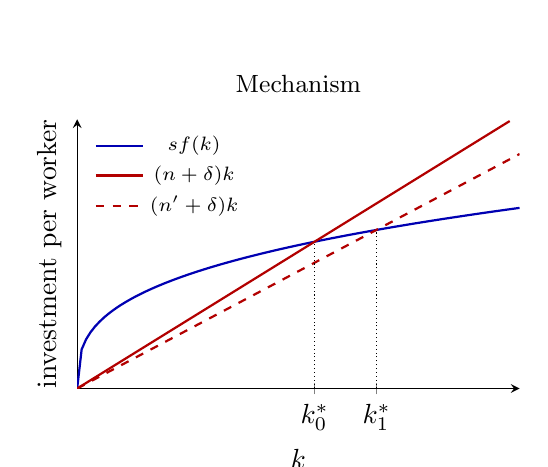
\begin{tikzpicture}
\begin{axis}[width=7.2cm,height=5cm,axis lines=left,xmin=0,xmax=9,ymin=0,ymax=0.62,
  xlabel={$k$},ylabel={investment per worker},xtick={4.83,6.09},xticklabels={$k^\ast_0$,$k^\ast_1$},
  ytick=\empty,title={\small Mechanism},legend style={font=\scriptsize,at={(0.02,0.98)},anchor=north west,draw=none}]
\addplot[thick,blue!70!black,domain=0:9,samples=100]{0.2*x^(1/3)};
\addplot[thick,red!70!black,domain=0:8.8]{0.07*x};
\addplot[thick,red!70!black,dashed,domain=0:9]{0.06*x};
\legend{$sf(k)$,$(n+\delta)k$,$(n'+\delta)k$}
\draw[densely dotted] (axis cs:4.83,0)--(axis cs:4.83,0.338);
\draw[densely dotted] (axis cs:6.09,0)--(axis cs:6.09,0.365);
\end{axis}
\end{tikzpicture}\quad
\begin{tikzpicture}
\begin{axis}[width=7.2cm,height=5cm,axis lines=left,xmin=-10,xmax=60,ymin=0.5,ymax=0.63,
  xlabel={time},ylabel={$\ln y$},xtick={0},xticklabels={$t_0$},ytick={0.525,0.602},
  yticklabels={$\ln y^\ast_0$,$\ln y^\ast_1$},title={\small Time path}]
\addplot[thick,blue!70!black,domain=-10:0]{0.5249};
\addplot[thick,blue!70!black,domain=0:60,samples=60]{0.6019-(0.6019-0.5249)*exp(-0.04*x)};
\addplot[densely dotted,domain=-10:60]{0.6019};
\end{axis}
\end{tikzpicture}
\end{center}
{\footnotesize Left: $n$ falls, the break-even ray rotates down, $k^\ast$ rises. Right: $\ln y$ rises
during the transition and flattens; $\ln Y$ (not drawn) has slope $n=2\%$ before and $n'=1\%$ after.}
\refbib{Kurlat ch.~4, \S4.2 (comparative statics), pp.~59--61.}
\end{sol}

\medskip
\textbf{b)} (3 points) Same model with $\alpha=0.35$ and $n+\delta=0.07$; Brazil saves 17\% of GDP.
Which statement is correct about the golden-rule saving rate and the effect on steady-state
consumption per worker of raising $s$ from 0.17 to 0.25?
\begin{alternativas}
\item $s_{GR}=0.65$; raising $s$ from 0.17 to 0.25 lowers steady-state consumption per worker.
\item $s_{GR}=0.35$; raising $s$ from 0.17 to 0.25 raises steady-state consumption per worker.
\item $s_{GR}=0.35$; raising $s$ from 0.17 to 0.25 lowers steady-state consumption per worker.
\item $s_{GR}=1.00$; raising $s$ from 0.17 to 0.25 raises steady-state consumption per worker.
\end{alternativas}
\gabarito{B.}
\begin{sol}
$c^\ast=f(k^\ast)-(n+\delta)k^\ast$ is maximised at $f'(k_{GR})=n+\delta$; with Cobb--Douglas
$\alpha k^{\alpha-1}=n+\delta$ and $s\,k^{\alpha-1}=n+\delta$ give $\boxed{s_{GR}=\alpha=0.35}$.
$c^\ast(s)=(1-s)\left(\frac{s}{0.07}\right)^{0.35/0.65}$: $c^\ast(0.17)=1.338<c^\ast(0.25)=1.488$.
Below the golden rule a higher $s$ raises long-run consumption (after an initial fall). A uses
$1-\alpha$; C reads only the $(1-s)$ factor; D maximises $k^\ast$, not $c^\ast$.
\refbib{Kurlat ch.~4, \S4.3 (golden rule), pp.~61--63.}
\end{sol}

\medskip
\textbf{c)} (2 points, T or F) Of two economies with the same technology, depreciation and population
growth, the one with lower capital per worker necessarily grows faster.
\gabarito{F.}
\begin{sol}
Convergence is \emph{conditional}: $g_k=s\,k^{\alpha-1}-(n+\delta)$ depends on the distance to each
economy's own steady state, which depends on $s$. With $\alpha=1/3$, $n+\delta=0.07$: $X$ with $k=3$,
$s=0.10$ has $g_k=-2.2\%$; $Z$ with $k=5$, $s=0.30$ has $g_k=+3.3\%$.
\refbib{Kurlat ch.~5, \S5.1--\S5.3 (convergence), pp.~75--86.}
\end{sol}

\medskip
\textbf{d)} (2 points, T or F) If a country's national accounts show a capital share of income of one
third, the same as in undistorted economies with $\alpha=1/3$, then its measured TFP reflects only
technology.
\gabarito{F.}
\begin{sol}
Normal factor shares do not rule out distortions. A requirement to hold unproductive capital recorded
as capital leaves $rK/Y=\alpha$ exactly and puts the whole distortion in the residual,
$\hat A=A(1+\theta)^{-\alpha}$ (Question 4).
\refbib{Kurlat ch.~5, \S5.4--\S5.5 (growth and development accounting), pp.~86--95.}
\gap{Lista 1, 4(b): a Solow comparative static in $n$ left blank; Lista 1, 4(a): aggregate vs per
capita (item a). Item (d) previews Lista 2, 2(c).}
\end{sol}

% -----------------------------------------------------------------------------
\questao{(15 points) ``Custo Brasil'' in the growth accounts.
Output is $Y=AK_P^{\alpha}L^{1-\alpha}$ with $\alpha=0.4$, where $K_P$ is productive capital.
Regulation, legal uncertainty and crime force every firm to hold $\theta$ units of \emph{compliance
capital} (duplicate tax-filing systems, armoured vehicles, walls, back-up generators) for each unit of
productive capital. Compliance capital produces nothing, but the national accounts record it as capital
like any other, so measured capital is $K=K_P+\theta K_P$. Capital is rented at $r$ and labour hired
at $w$ in competitive markets. Today $\theta=0.6$.}

\textbf{a)} (5 points) Write aggregate output as a function of $A,K,L,\theta$. What share of measured
capital is unproductive? How much output is lost relative to an economy with $\theta=0$ and the same
$A,K,L$? State the base of your percentage.
\resolespaco
\begin{sol}
\passo{1 --- composition}{$K=(1+\theta)K_P\Rightarrow K_P=K/(1+\theta)$.}
\passo{2 --- output}{$Y=A\left(\dfrac{K}{1+\theta}\right)^{\alpha}L^{1-\alpha}
\;\Rightarrow\;\boxed{Y=\underbrace{A(1+\theta)^{-\alpha}}_{\text{wedge on TFP}}K^{\alpha}L^{1-\alpha}}$.}
\passo{3 --- unproductive share}{$\dfrac{\theta K_P}{(1+\theta)K_P}=\dfrac{0.6}{1.6}=\boxed{37.5\%}$.}
\passo{4 --- output lost}{$\dfrac{Y(\theta)}{Y(0)}=(1.6)^{-0.4}=e^{-0.4\ln1.6}=e^{-0.4\cdot0.4700}=e^{-0.1880}=0.8286$.
\boxed{\text{Output is }17.1\%\text{ below the undistorted level}} (base: $Y(0)$). Equivalently,
removing $\theta$ would raise output by $1/0.8286-1=\boxed{20.7\%}$ (base: $Y(\theta)$).
\#~Careful with the chosen base.}
\intuicao{A third of the capital stock does no work, but output falls by less than a third because
capital has diminishing returns and a share of only 0.4.}
\refbib{Kurlat ch.~5, \S5.4--\S5.5, pp.~86--95.}
\rubrica{
\item $K_P=K/(1+\theta)$ and the boxed $Y$ with the wedge named: 2 pts.
\item Share 37.5\%: 1 pt.
\item Loss 17.1\% (or gain 20.7\%) with the base stated: 2 pts; no base stated: $-1$ pt.
\item Loss computed as $\theta/(1+\theta)=37.5\%$ of output: max.\ 2 pts on the item.
}
\end{sol}

\textbf{b)} (5 points) Write the representative firm's problem and first-order conditions and derive
the measured factor shares $rK/Y$ and $wL/Y$. A development accountant has data on $Y$, $K$, $L$ and
factor payments only. What does she conclude about $\alpha$ and about TFP? Who bears the cost of
$\theta$?
\resolespaco
\begin{sol}
\passo{1 --- problem}{To use $K_P$ productive units the firm must rent $(1+\theta)K_P$:
$\max_{K_P,L}\;AK_P^{\alpha}L^{1-\alpha}-r(1+\theta)K_P-wL$.}
\passo{2 --- FOCs}{$\alpha\dfrac{Y}{K_P}=r(1+\theta)$ and $(1-\alpha)\dfrac{Y}{L}=w$.}
\passo{3 --- shares}{Using $(1+\theta)K_P=K$: $r=\dfrac{\alpha Y}{(1+\theta)K_P}=\alpha\dfrac{Y}{K}$, so
$\boxed{rK/Y=\alpha=0.4}$ and $\boxed{wL/Y=1-\alpha=0.6}$: \emph{undistorted}.}
\passo{4 --- the accountant}{She sets $\hat\alpha=rK/Y=0.4=\alpha$ (correct) and computes
$\hat A=\dfrac{Y}{K^{\hat\alpha}L^{1-\hat\alpha}}=\boxed{A(1+\theta)^{-\alpha}=0.83A}$.
She concludes that Brazil has 17\% lower \emph{technology}. Wrong: technology is $A$; the gap is a
wasted-capital distortion that the data classify as productivity.}
\passo{5 --- incidence}{The rental rate $r=\alpha Y/K$ and the wage
$w=(1-\alpha)\hat A(K/L)^{\alpha}$ are both lower at given $K/L$ by the factor $(1+\theta)^{-\alpha}$.
\#~Workers are also affected: capital and labour are complements.}
\intuicao{Each productive machine drags $\theta$ idle ones with it, so capital looks less productive
by exactly the amount it is paid less: the share is untouched, the level is not.}
\refbib{Kurlat ch.~5, \S5.4 (factor shares and TFP), pp.~86--92.}
\rubrica{
\item Problem with cost $r(1+\theta)K_P$ and both FOCs: 1.5 pts.
\item $rK/Y=\alpha$, $wL/Y=1-\alpha$: 1.5 pts.
\item $\hat\alpha=\alpha$ and $\hat A=A(1+\theta)^{-\alpha}$, read as distortion, not technology: 1.5 pts.
\item Workers also bear the cost: 0.5 pt.
\item Claiming the capital share is distorted ($\hat\alpha\neq\alpha$): max.\ 2 pts on the item.
}
\end{sol}

\textbf{c)} (5 points) A reform (tax simplification, digital filing, lower crime) cuts $\theta$ from
0.6 to 0.28 gradually over the decade 2027--2036, while true $A$ stays constant; $K$ and $L$ grow at
whatever rates they grow. Write the growth-accounting decomposition, compute the average annual Solow
residual, say what it would show if $\theta$ instead \emph{rose} from 0.28 to 0.6, and explain why
this is consistent with Kurlat's reading of the residual.
\resolespaco
\begin{sol}
\passo{1 --- decomposition}{From $Y_t=A(1+\theta_t)^{-\alpha}K_t^{\alpha}L_t^{1-\alpha}$, in logs over the decade:
$\Delta\ln Y=\alpha\,\Delta\ln K+(1-\alpha)\Delta\ln L+\underbrace{\Delta\ln A}_{=0}\underbrace{-\alpha\,\Delta\ln(1+\theta)}_{\Delta\theta}$.
The accountant computes $\text{residual}=\Delta\ln Y-\alpha\Delta\ln K-(1-\alpha)\Delta\ln L=\underbrace{g_{\text{TFP}}+\Delta\theta\text{ term}}_{\text{Solow residual}}$.}
\passo{2 --- number}{$\alpha\ln\dfrac{1+\theta}{1+\theta'}=0.4\ln\dfrac{1.6}{1.28}=0.4\ln1.25=0.4\cdot0.2231=0.0893$
over ten years, i.e.\ $\boxed{\approx0.89\text{ pp per year}}$ of measured ``TFP growth'' with zero
technical progress. $\ln\hat A$ goes from $-0.188$ to $-0.099$.}
\passo{3 --- the reverse}{If $\theta$ rose from 0.28 to 0.6 the residual would be
$\boxed{-0.89\text{ pp per year}}$: measured technological regress with unchanged technology.}
\passo{4 --- check}{$K$ and $L$ are subtracted with the right weights (shares are undistorted, (b)),
so the $\theta$ effect lands entirely in the residual whatever $K$ and $L$ do.}
\passo{5 --- Kurlat's reading}{The residual is whatever output growth the measured inputs do not
explain --- ``a measure of our ignorance''. It contains technology \emph{and} the efficiency with which
measured inputs are used (regulation, institutions, misallocation). A falling $\theta$ is exactly an
efficiency gain in the use of measured capital, so it belongs in the residual.}
\begin{center}
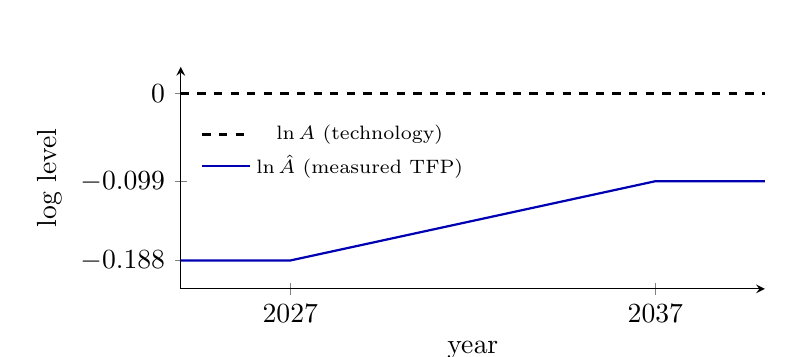
\begin{tikzpicture}
\begin{axis}[width=9cm,height=4.4cm,axis lines=left,xmin=2024,xmax=2040,ymin=-0.22,ymax=0.03,
  xlabel={year},ylabel={log level},xtick={2027,2037},xticklabels={2027,2037},
  ytick={-0.188,-0.099,0},yticklabels={$-0.188$,$-0.099$,$0$},
  legend style={font=\scriptsize,at={(0.02,0.62)},anchor=west,draw=none},
  x tick label style={/pgf/number format/1000 sep=}]
\addplot[thick,dashed,black,domain=2024:2040]{0};
\addplot[thick,blue!70!black] coordinates {(2024,-0.188) (2027,-0.188) (2037,-0.0987) (2040,-0.0987)};
\legend{$\ln A$ (technology),$\ln\hat A$ (measured TFP)}
\end{axis}
\end{tikzpicture}\\
{\footnotesize Measured TFP rises 0.89 pp a year during the reform and stops when $\theta$ stops falling; true $A$ never moves.}
\end{center}
\intuicao{The reform does not invent anything; it releases capital that was already paid for. The
data see more output from the same measured inputs and call it productivity.}
\refbib{Kurlat ch.~5, \S5.4--\S5.5 (growth accounting and what the residual contains), pp.~86--95.}
\rubrica{
\item Decomposition with the residual split into $g_{\text{TFP}}$ and the $\theta$ term: 1.5 pts.
\item $0.4\ln1.25=0.089$, about 0.89 pp per year: 1.5 pts (arithmetic slip: $-1$ pt).
\item Reverse case with the sign: 1 pt.
\item Kurlat's reading of the residual: 1 pt.
\item Residual set to zero ``because $A$ is constant'': max.\ 1 pt on the item.
}
\gap{Lista 2, 2(d), left blank: the growth-accounting residual when a capital-wasting distortion
falls. Items (a)--(c) of Lista 2 were right; this question re-asks (d) with new numbers.}
\end{sol}

% =============================================================================
\bloco{III}{Microfoundations: consumption, labour and general equilibrium}{Lectures 4--6 \,\textbullet\, 25 points}

\questao{(10 points) Objective items.}

\textbf{a)} (3 points) A two-period household (Kurlat ch.~6) has $u=\ln c_1+\beta\ln c_2$ with
$\beta=1$, faces $r=0$, can borrow and lend freely and earns $y_1=y_2=10{,}000$ reais. Consider three
separate scenarios, each against this baseline: (i) a one-off bonus of 1{,}000 today (an extraordinary
FGTS withdrawal); (ii) a credible announcement today of a raise of 1{,}000 paid in period 2 only;
(iii) a permanent raise of 1{,}000 in both periods. The changes in $c_1$ in (i), (ii), (iii) are:
\begin{alternativas}
\item 1{,}000; \ 0; \ 1{,}000
\item 500; \ 0; \ 1{,}000
\item 500; \ 500; \ 1{,}000
\item 500; \ 500; \ 500
\item 1{,}000; \ 500; \ 2{,}000
\end{alternativas}
\gabarito{C.}
\begin{sol}
With log utility $c_1=\dfrac{y_1+y_2/(1+r)}{1+\beta}=\dfrac{y_1+y_2}{2}$. (i) $\Delta W=1{,}000\Rightarrow\Delta c_1=500$;
(ii) $\Delta W=1{,}000/(1+0)=1{,}000\Rightarrow\Delta c_1=500$: news about future income moves
consumption \emph{today}, financed by borrowing; (iii) $\Delta W=2{,}000\Rightarrow\Delta c_1=1{,}000$.
\boxed{500;\ 500;\ 1{,}000}. A is Keynesian (current income only); B ignores the news.
\refbib{Kurlat ch.~6, \S6.2--\S6.3 (permanent income), pp.~105--120.}
\end{sol}

\medskip
\textbf{b)} (3 points) The government must raise a given revenue from households that save. It can tax
interest income or levy a lump-sum tax in period 2 that raises the same revenue. With CRRA utility,
which statement is correct?
\begin{alternativas}
\item Only the tax on interest changes $c_2/c_1$, through the net return in the Euler equation; at equal revenue the lump sum gives higher utility.
\item Both taxes lower $c_2/c_1$ by the same amount, because they raise the same revenue in present value and so lower wealth equally.
\item Only the lump-sum tax changes $c_2/c_1$, because it lowers wealth; the tax on interest is neutral once its revenue is fixed.
\item Only the tax on interest changes $c_2/c_1$, through the net return in the Euler equation; at equal revenue both give the same utility.
\end{alternativas}
\gabarito{A.}
\begin{sol}
Euler: $u'(c_1)=\beta[1+r(1-\tau)]u'(c_2)\Rightarrow c_2/c_1=\{\beta[1+r(1-\tau)]\}^{1/\sigma}$: the
\emph{intertemporal margin} is distorted. The lump sum shifts the budget line in parallel and leaves
$c_2/c_1=[\beta(1+r)]^{1/\sigma}$. At equal revenue $T=\tau ra$, the plan chosen under the interest tax
costs exactly $y_1+(y_2-T)/(1+r)$ at market prices, so it was affordable under the lump sum and not
chosen: \boxed{U^{\text{lump sum}}>U^{\text{interest tax}}}, the difference being deadweight loss
(D misses this).
\refbib{Kurlat ch.~6, \S6.2--\S6.4 (taxes in the two-period model), pp.~105--126.}
\end{sol}

\medskip
\textbf{c)} (2 points, T or F) A household with $u=\ln c_1+\beta\ln c_2$ earns $y_1>0$ in period 1 and
nothing in period 2 (no taxes), so it is a net saver. When $r$ rises it raises $c_1$, because for a
saver the income effect of a higher return dominates the substitution effect.
\gabarito{F.}
\begin{sol}
$c_1=\dfrac{y_1}{1+\beta}$, independent of $r$: with $\sigma=1$ and no future income to revalue, the
income and substitution effects cancel \emph{exactly}. The sign of $\partial c_1/\partial r$ is that
of $\sigma-1$; the income effect wins only if $\sigma>1$.
\refbib{Kurlat ch.~6, \S6.2 (the effect of interest rates), pp.~108--115.}
\end{sol}

\medskip
\textbf{d)} (2 points, T or F) With $u=\ln c-\chi\,h^{1+\eta}/(1+\eta)$ and no non-labour income, hours
do not respond to a permanent change in the wage (the Marshallian elasticity is zero). Therefore a
temporary, anticipated wage rise within a life of given wealth leaves hours unchanged too: the Frisch
elasticity is also zero.
\gabarito{F.}
\begin{sol}
Marshallian: $\chi h^{\eta}=w/c=w/(wh)=1/h$, hours constant. Frisch (marginal utility of wealth
$\mu$ fixed): $\chi h^{\eta}=\mu w\Rightarrow\varepsilon^F=1/\eta>0$. The ordering is
$\varepsilon^F\ge\varepsilon^H\ge\varepsilon^M$; a zero Marshallian elasticity means two effects
cancel, not that labour supply is unresponsive.
\refbib{Kurlat ch.~7, \S7.3--\S7.4, pp.~137--142.}
\gap{Lista 3, 1(b): no permanent-income story for a rise in expected $y_2$ (item a). Lista 3, 2(d): the
equal-revenue lump-sum comparison and the distorted margin were never stated (item b).}
\end{sol}

% -----------------------------------------------------------------------------
\questao{(15 points) An agribusiness productivity boom in general equilibrium.
A one-period economy has a fixed capital stock $\bar K$. The representative household owns $\bar K$ and
the firm, has one unit of time and utility $u=\dfrac{c^{1-\sigma}}{1-\sigma}+\psi\ln(1-L)$ with
$\psi=2/3$ ($\sigma$ is the curvature of utility; $1/\sigma$ the elasticity of substitution).
The competitive firm produces $Y=A\bar K^{\alpha}L^{1-\alpha}$ with $\alpha=1/3$. At the baseline
$A\bar K^{\alpha}=2^{2/3}$ and $\sigma=2$. New seed varieties raise $A$ in agriculture, which we treat
as a rise in aggregate $A$.}

\textbf{a)} (5 points) Write the household's and the firm's problems, the first-order conditions and the
market-clearing conditions. Show that profits are zero. Reduce the equilibrium to one equation in $L$,
verify that $L=1/2$ at the baseline, and compute $c$, $w$ and $r^K\bar K$.
\resolespaco
\begin{sol}
\passo{1 --- household}{$\max_{c,L}\ \frac{c^{1-\sigma}}{1-\sigma}+\psi\ln(1-L)$ s.t.\
$c=wL+r^K\bar K+\Pi$. FOC: $\boxed{\dfrac{\psi}{1-L}=w\,c^{-\sigma}}$ (MRS between leisure and
consumption $=$ real wage).}
\passo{2 --- firm}{$\max_L\ A\bar K^{\alpha}L^{1-\alpha}-wL-r^K\bar K$:
$w=(1-\alpha)\dfrac{Y}{L}$ (MPL), $r^K=\alpha\dfrac{Y}{\bar K}$ (MPK).
$\Pi=Y-(1-\alpha)Y-\alpha Y=0$ (constant returns, Euler's theorem).}
\passo{3 --- clearing}{Goods: $c=Y$ (no investment, no government). Capital: supply fixed at $\bar K$.}
\passo{4 --- one equation}{Let $\tilde A=A\bar K^{\alpha}$, so $c=\tilde AL^{1-\alpha}$ and
$w=(1-\alpha)\tilde AL^{-\alpha}$. Substituting into Step 1:
$\boxed{\psi\dfrac{L^{\alpha+(1-\alpha)\sigma}}{1-L}=(1-\alpha)\tilde A^{1-\sigma}}$ (MRS $=$ MPL).
The left side rises in $L$, so the solution is unique.}
\passo{5 --- verify}{$\sigma=2$: exponent $\tfrac13+\tfrac43=\tfrac53$. LHS at $L=\tfrac12$:
$\tfrac23\cdot\dfrac{2^{-5/3}}{2^{-1}}=\tfrac23\,2^{-2/3}$. RHS: $\tfrac23(2^{2/3})^{-1}=\tfrac23\,2^{-2/3}$ \checkmark.
Then $\boxed{c=Y=2^{2/3}\,2^{-2/3}=1}$, $\boxed{w=\tfrac23\cdot1/\tfrac12=\tfrac43}$,
$\boxed{r^K\bar K=\tfrac13}$; check $wL+r^K\bar K=\tfrac23+\tfrac13=1=Y$.}
\refbib{Kurlat ch.~9, \S9.1--\S9.2 (competitive equilibrium), pp.~165--180; ch.~7, \S7.2.}
\rubrica{
\item Both problems and FOCs, including MRS $=w$: 2 pts.
\item Zero profits and $c=Y$: 1 pt.
\item Equation in $L$ and the baseline check with $c,w,r^K\bar K$: 2 pts.
\item Adding the principal $\bar K$ to household income: $-1$ pt (budget no longer matches $c=Y$).
}
\end{sol}

\textbf{b)} (5 points) Derive $d\ln L/d\ln A$ in general and sign it by $\sigma$. Evaluate it at the
baseline and give the first-order effects of a 10\% rise in $A$ on $L$, $w$, $r^K$ and $c$. Explain in
words that match the sign.
\resolespaco
\begin{sol}
\passo{1 --- differentiate}{Log of the equation in (a):
$\ln\psi+[\alpha+(1-\alpha)\sigma]\ln L-\ln(1-L)=\ln(1-\alpha)+(1-\sigma)\ln\tilde A$.
Differentiating, with $d\ln\tilde A=d\ln A$:
$\boxed{\dfrac{d\ln L}{d\ln A}=\dfrac{1-\sigma}{\alpha+(1-\alpha)\sigma+\frac{L}{1-L}}}$.}
\passo{2 --- sign}{The denominator is positive, so the sign is that of $1-\sigma$:
$\sigma<1\Rightarrow L\uparrow$; $\sigma=1\Rightarrow L$ unchanged; $\sigma>1\Rightarrow L\downarrow$.}
\passo{3 --- baseline}{$\sigma=2$, $L=\tfrac12$: $\dfrac{-1}{\frac13+\frac43+1}=\dfrac{-1}{8/3}=\boxed{-0.375}$.}
\passo{4 --- 10\% boom}{$d\ln L=-3.75\%$. $d\ln w=d\ln A-\alpha\,d\ln L=10+\tfrac13(3.75)=\boxed{+11.25\%}$.
$d\ln r^K=d\ln A+(1-\alpha)d\ln L=10-\tfrac23(3.75)=\boxed{+7.5\%}$.
$d\ln c=d\ln Y=d\ln A+(1-\alpha)d\ln L=\boxed{+7.5\%}$.}
\passo{5 --- words}{$A\uparrow\rightarrow w\uparrow$: leisure is dearer (substitution effect, work more)
but the household is richer (income effect, enjoy more leisure). With $\sigma=2$ marginal utility of
consumption falls fast as $c$ rises, so the \emph{income effect dominates} and hours fall. Output and
consumption still rise, by less than $A$.}
\intuicao{$\sigma$ measures how fast extra consumption loses value. Above one, a richer household
prefers to take part of its gain as leisure; at exactly one the two effects cancel.}
\refbib{Kurlat ch.~7, \S7.2 (income and substitution effects), pp.~131--137; ch.~9, \S9.2.}
\rubrica{
\item Correct derivative: 2 pts. Sign by $\sigma$ with the three cases: 1 pt.
\item $-0.375$ and the four effects: 1 pt (arithmetic slip: $-1$ pt, non-cumulative).
\item Words matching the sign: 1 pt.
\item Words describing only the substitution effect (``higher wage, so they work more'') when the derivative is negative: max.\ 3 pts on the item.
}
\end{sol}

\textbf{c)} (5 points) Now set $\sigma=1$. The government taxes labour income at $\tau=0.25$.
Compute equilibrium hours without the tax and in two cases: (i) the revenue is rebated lump sum;
(ii) the revenue is thrown away (spent on something with no value to the household). Explain why hours
fall in (i) even with log utility, why they fall less in (ii), and what happens in (ii) if $\alpha\to0$.
\resolespaco
\begin{sol}
\passo{1 --- FOC with the tax}{Budget $c=(1-\tau)wL+r^K\bar K+T$; FOC
$\dfrac{\psi}{1-L}=\dfrac{(1-\tau)w}{c}$, with $w=(1-\alpha)Y/L$.}
\passo{2 --- no tax}{$c=Y$: $\psi\dfrac{L}{1-L}=1-\alpha\Rightarrow\tfrac23\dfrac{L}{1-L}=\tfrac23\Rightarrow\boxed{L=\tfrac12}$.}
\passo{3 --- (i) rebate}{$T=\tau wL\Rightarrow c=Y$:
$\psi\dfrac{L}{1-L}=(1-\tau)(1-\alpha)=0.75\cdot\tfrac23=0.5\Rightarrow
L=\dfrac{0.5}{\frac23+0.5}=\boxed{\tfrac37\approx0.429}$.}
\passo{4 --- (ii) thrown away}{$c=Y-\tau wL=Y[1-\tau(1-\alpha)]$:
$\psi\dfrac{L}{1-L}=\dfrac{(1-\tau)(1-\alpha)}{1-\tau(1-\alpha)}=\dfrac{0.5}{5/6}=0.6\Rightarrow
\dfrac{L}{1-L}=0.9\Rightarrow\boxed{L=\tfrac{9}{19}\approx0.474}$.}
\passo{5 --- why (i) falls}{The rebate hands back the revenue: total income is unchanged ($c=Y$) but the
price of leisure falls to $(1-\tau)w$. The transfer is non-labour income that does not shrink with
the net wage, so the tax acts as a \emph{compensated} wage cut: a pure substitution effect $\Rightarrow$
hours fall, with log utility or not.}
\passo{6 --- why (ii) falls less, and $\alpha\to0$}{Without the rebate the household is poorer. On
labour income, log utility makes the income and substitution effects cancel; only the capital rents
$r^K\bar K$ (share $\alpha$), unearned income that does not fall with the net wage, leave a residual
effect. As $\alpha\to0$ the right side tends to $(1-\tau)/(1-\tau)=1$ and
\boxed{L\text{ is independent of }\tau}.}
\intuicao{With log consumption utility, a wage tax changes hours only through non-labour income ---
the transfer and the capital rents. Set that income to zero and the effect vanishes; the story must
therefore be about the transfer.}
\refbib{Kurlat ch.~7, \S7.2 (taxes and labour supply), pp.~131--137; ch.~9, \S9.2.}
\rubrica{
\item FOC with $(1-\tau)w$: 1 pt. $L=\tfrac12$, $\tfrac37$, $\tfrac{9}{19}$: 2 pts (slip: $-1$ pt).
\item Rebate $=$ compensated change, substitution effect only: 1 pt.
\item Role of non-labour income in (ii) and the $\alpha\to0$ limit: 1 pt.
\item Explaining (i) by ``the tax lowers the wage, so leisure is cheaper'' with no role for the transfer, and claiming the same in (ii): max.\ 2 pts on the item.
}
\gap{Lista 4, 1(b): with log utility labour responds to a wage tax only through the transfer, but the
words described the substitution effect. Lista 5, Q1: the sign of $d\ln L/d\ln A$ is that of
$1-\sigma$ and the words must match it.}
\end{sol}

% =============================================================================
\bloco{IV}{Money, inflation and the New-Keynesian AS--AD model}{Lectures 7--9 \,\textbullet\, 25 points}

\questao{(10 points) Objective items.}

\textbf{a)} (3 points) A flexible-price economy (Kurlat ch.~11) has real money demand $M/P=Y\,\ell(i)$,
$\ell'<0$, with $Y$ and $r$ fixed by the real side. Which statement is correct?
\begin{alternativas}
\item A one-off 10\% rise in $M$ raises $P$ by 10\% and leaves $Y$, $r$ and $M/P$ unchanged; a permanent rise in money growth also leaves $M/P$ unchanged, as money is superneutral.
\item A one-off 10\% rise in $M$ raises $P$ by 10\% and leaves $Y$, $r$ and $M/P$ unchanged; a permanent rise in money growth raises $i$ and lowers $M/P$.
\item A one-off 10\% rise in $M$ lowers $i$ through a liquidity effect and raises $Y$ for good; a permanent rise in money growth raises $i$ and lowers $M/P$.
\item A one-off 10\% rise in $M$ raises $P$ by 10\% and leaves $Y$, $r$ and $M/P$ unchanged; under a Selic target the Copom fixes both $i$ and $M$ independently.
\end{alternativas}
\gabarito{B.}
\begin{sol}
Level change: neutrality, $P$ moves one for one. Growth change: $\pi\uparrow\Rightarrow i=r+\pi\uparrow
\Rightarrow\ell(i)\downarrow$: money is neutral but \emph{not superneutral} (A). C is IS--LM with
flexible prices. D: with $i$ as the instrument, $M=P\,Y\ell(\bar\imath)$ is \emph{determined} by the
money market; the bank cannot also choose $M$.
\refbib{Kurlat ch.~11, \S11.1--\S11.2, pp.~205--215; ch.~10 on the instrument.}
\end{sol}

\medskip
\textbf{b)} (3 points) Real money demand is $M/P=0.10\,Y\,e^{-4\pi}$ (Cagan form, $\pi$ in decimal per
year), $Y$ is constant and in steady state $\pi$ equals money growth. The inflation rate that maximises
seigniorage, and seigniorage at that rate, are:
\begin{alternativas}
\item $\pi=12.5\%$; seigniorage $0.76\%$ of GDP
\item $\pi=25\%$; seigniorage $2.50\%$ of GDP
\item $\pi=50\%$; seigniorage $0.68\%$ of GDP
\item $\pi=25\%$; seigniorage $0.92\%$ of GDP
\end{alternativas}
\gabarito{D.}
\begin{sol}
$S/Y=\pi\cdot0.10e^{-4\pi}$; $\frac{d}{d\pi}=0.10e^{-4\pi}(1-4\pi)=0\Rightarrow\boxed{\pi=1/a=25\%}$;
$S/Y=0.25\cdot0.10\cdot e^{-1}=\boxed{0.92\%}$. B ignores the erosion of the base ($0.25\times0.10$);
A and C are off the peak ($0.76\%$, $0.68\%$).
\refbib{Kurlat ch.~11, \S11.3 (seigniorage) and Exercise 11.6 (Cagan), pp.~215--222.}
\end{sol}

\medskip
\textbf{c)} (2 points, T or F) In Benigno's AS--AD model, a cut in the Selic moves the economy along the
AS curve.
\gabarito{T.}
\begin{sol}
$i$ enters only AD. The cut shifts AD up and to the right; AS (anchored at $(p^e,y_n)$) does not move,
so the new equilibrium lies further up the same AS: $y\uparrow$, $p\uparrow$.
\refbib{Benigno (2015), \S5, Figs.~3--5, pp.~509--511.}
\end{sol}

\medskip
\textbf{d)} (2 points, T or F) In Benigno's model, natural output $y_n$ differs from efficient output
$y_e$ because a fraction of prices is sticky.
\gabarito{F.}
\begin{sol}
$y_n$ is the flexible-price equilibrium, $y_e$ the planner's choice; the stickiness share $\alpha$ is
in neither. The gap is the mark-up wedge (market power and taxes): $y_n-y_e=-\mu/(\sigma^{-1}+\eta)$.
Stickiness explains $y\neq y_n$.
\refbib{Benigno (2015), \S4.2--\S4.4, eqs.~(15), (19), pp.~508--509.}
\gap{Lista 6, 1(c)--(d): flexible prices $\Rightarrow$ neutrality; under an interest-rate instrument
the money market determines $M$ (item a). Lista 7 traps 1 and 4 (items c, d).}
\end{sol}

% -----------------------------------------------------------------------------
\questao{(15 points) A mark-up shock in fuel distribution.
A merger wave concentrates fuel distribution and raises firms' desired mark-up by 4.4\% for one period
only. Use Benigno's model in log deviations from an efficient steady state, with no public spending
($g=0$), no tax changes, $\bar p=p^e=0$ and $\bar y_n=0$:
\[
\text{AS: } p-p^e=\kappa(y-y_n),\quad \kappa=\frac{(1-\alpha)(\sigma^{-1}+\eta)}{\alpha};\qquad
\text{AD: } y=\bar y_n-\sigma\left[i-(\bar p-p)-\rho\right].
\]
Calibration: $\alpha=0.66$ (share of sticky prices), $\sigma=0.5$, $\eta=0.2$, $\theta=8$, $\rho=5\%$.
Before the shock $i=\rho$, $y=y_n=y_e=0$ and $p=p^e$. At first the Copom keeps the Selic at 5\%.}

\textbf{a)} (5 points) Which curve shifts and which does not, and why? Find $y$ and $p$, and the signs
of $y-y_n$ and $y-y_e$. Draw the AS--AD diagram and the time path of $y$ and $p$ over the short run
(period 1) and the long run (period 2).
\resolespaco
\begin{sol}
\passo{1 --- slope}{$\kappa=\dfrac{0.34\cdot(2+0.2)}{0.66}=\dfrac{0.748}{0.66}=1.133$; $\sigma\kappa=0.567$.}
\passo{2 --- what shifts}{$y_n=\dfrac{(1+\eta)a-\mu}{\sigma^{-1}+\eta}\Rightarrow dy_n=-\dfrac{4.4}{2.2}=\boxed{-2\%}$;
$y_e$ has no $\mu$, $dy_e=0$. \boxed{\text{AS shifts up/left}} through $(p^e,y_n'=-2)$, by
$\kappa\cdot2=2.27$ pp at given $y$ ($=\frac{1-\alpha}{\alpha}d\mu=0.515\cdot4.4$ \checkmark).
\boxed{\text{AD does not shift}}: $\mu$ is not in AD, $i$ is unchanged, and a \emph{temporary} shock leaves $\bar y_n$ unchanged.}
\passo{3 --- equilibrium}{AD with $i=\rho$: $p=-y/\sigma=-2y$. AS: $p=1.133(y+2)$.
$-2y=1.133y+2.267\Rightarrow y=-\dfrac{2.267}{3.133}=\boxed{-0.72\%}$, $\boxed{p=+1.45\%}$: stagflation.
(Closed form: $dy=\frac{\sigma\kappa}{1+\sigma\kappa}dy_n$, $dp=-\frac{\kappa}{1+\sigma\kappa}dy_n$.)}
\passo{4 --- two gaps}{$\boxed{y-y_n=-0.72+2=+1.28>0}$ (why prices rise: AS responds to $y-y_n$);
$\boxed{y-y_e=-0.72<0}$ (why welfare falls).}
\passo{5 --- chain}{$\mu\uparrow\rightarrow$ adjusting firms raise prices $\rightarrow p\uparrow
\rightarrow$ real rate $i-(\bar p-p)\uparrow\rightarrow c\downarrow\rightarrow y\downarrow$ along AD.
LR: the shock is over, all firms reset, $y=\bar y_n=0$, $p=\bar p=0$.}
\begin{center}
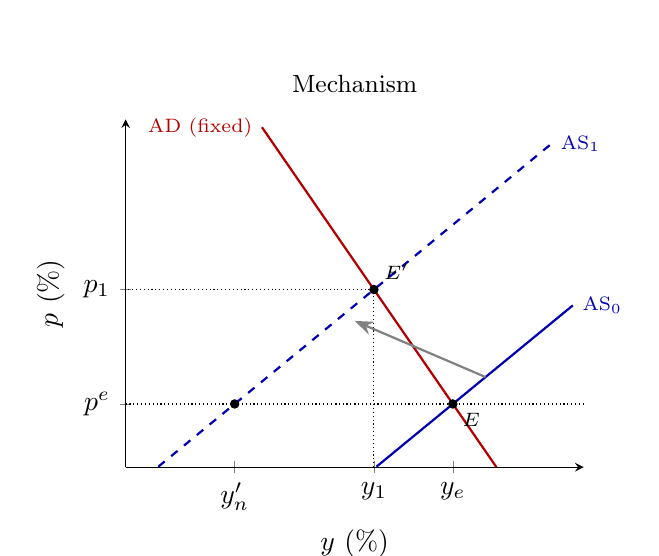
\begin{tikzpicture}
\begin{axis}[width=7.4cm,height=6cm,axis lines=left,xmin=-3,xmax=1.2,ymin=-0.8,ymax=3.6,clip=false,
  xlabel={$y$ (\%)},ylabel={$p$ (\%)},xtick={-2,-0.7234,0},xticklabels={$y_n'$,$y_1$,$y_e$},
  ytick={0,1.4468},yticklabels={$p^e$,$p_1$},title={\small Mechanism}]
\addplot[densely dotted,domain=-3:1.2]{0};
\addplot[thick,blue!70!black,domain=-0.7:1.1]{1.1333*x};
\addplot[thick,blue!70!black,dashed,domain=-2.7:0.9]{1.1333*(x+2)};
\addplot[thick,red!70!black,domain=-1.75:0.4]{-2*x};
\node[font=\scriptsize,blue!70!black,anchor=west] at (axis cs:1.1,1.25) {AS$_0$};
\node[font=\scriptsize,blue!70!black,anchor=west] at (axis cs:0.9,3.29) {AS$_1$};
\node[font=\scriptsize,red!70!black,anchor=east] at (axis cs:-1.75,3.5) {AD (fixed)};
\addplot[only marks,mark=*,mark size=1.5pt] coordinates {(0,0) (-0.7234,1.4468) (-2,0)};
\node[font=\scriptsize,anchor=north west] at (axis cs:0,0) {$E$};
\node[font=\scriptsize,anchor=south west] at (axis cs:-0.72,1.45) {$E'$};
\draw[densely dotted] (axis cs:-0.7234,-0.8)--(axis cs:-0.7234,1.4468)--(axis cs:-3,1.4468);
\draw[-{Stealth},thick,gray] (axis cs:0.3,0.34)--(axis cs:-0.9,1.05);
\end{axis}
\end{tikzpicture}\quad
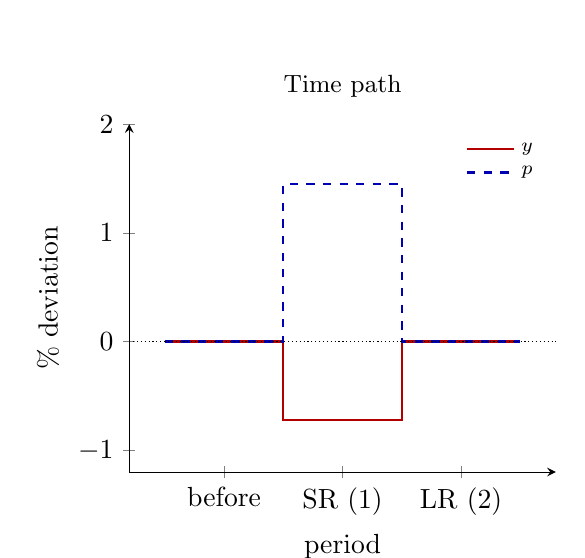
\begin{tikzpicture}
\begin{axis}[width=7cm,height=6cm,axis lines=left,xmin=-0.3,xmax=3.3,ymin=-1.2,ymax=2,
  xlabel={period},xtick={0.5,1.5,2.5},xticklabels={before,SR (1),LR (2)},ylabel={\% deviation},
  title={\small Time path},legend style={font=\scriptsize,draw=none,at={(0.98,0.98)},anchor=north east}]
\addplot[thick,red!70!black,const plot] coordinates {(0,0) (1,-0.7234) (2,0) (3,0)};
\addplot[thick,blue!70!black,dashed,const plot] coordinates {(0,0) (1,1.4468) (2,0) (3,0)};
\addplot[densely dotted,domain=-0.3:3.3]{0};
\legend{$y$,$p$}
\end{axis}
\end{tikzpicture}
\end{center}
\intuicao{The mark-up raises prices at any output; with $\bar p$ anchored, a higher $p$ is a higher real
rate, so demand falls along AD. Output does not fall all the way to $y_n'$ because the sticky firms keep
selling at $p^e$.}
\refbib{Benigno (2015), \S7, Fig.~9, pp.~513--514; \S5, eqs.~(20)--(21).}
\rubrica{
\item AS shifts up/left and AD explicitly does \emph{not} move, with reasons: 1.5 pts.
\item $y=-0.72$, $p=+1.45$: 1 pt (slip: $-1$ pt).
\item Both gaps with opposite signs: 1 pt.
\item Diagram: axes, AS$_0$, AS$_1$ and the unmoved AD labelled, direction of shift: 1 pt; time path SR/LR: 0.5 pt.
\item Shifting AD: max.\ 2 pts on the item. Reporting a single ``output gap'': max.\ 3.5 pts.
}
\end{sol}

\textbf{b)} (5 points) With $u(C)=\dfrac{C^{1-1/\sigma}}{1-1/\sigma}$, $v(L)=\dfrac{L^{1+\eta}}{1+\eta}$,
$Y=AL$ and $C=Y$, the market's labour-supply condition is $\text{MRS}=A/(1+\mu)$ and the planner's is
$\text{MRS}=A$. Derive both, log-linearise, and show $y_n-y_e=-\mu/(\sigma^{-1}+\eta)$. Explain why sticky
prices play no role, and evaluate the gap for this shock.
\resolespaco
\begin{sol}
\passo{1 --- planner}{$\max_Y u(Y)-v(Y/A)$: $u'(Y)=v'(L)/A\Rightarrow\boxed{\dfrac{v'(L)}{u'(C)}=A}$
(MRS $=$ MRT).}
\passo{2 --- market}{Flexible-price firms set $P=(1+\mu)W/A\Rightarrow W/P=A/(1+\mu)$; the household sets
MRS $=W/P$: $\boxed{\dfrac{v'(L)}{u'(C)}=\dfrac{A}{1+\mu}}$. Same condition up to the wedge $1+\mu$.}
\passo{3 --- logs}{$\ln v'=\eta l=\eta(y-a)$; $\ln u'=-\sigma^{-1}c=-\sigma^{-1}y$. So
$\ln\text{MRS}=\eta(y-a)+\sigma^{-1}y$. Planner: $=a\Rightarrow y_e=\dfrac{(1+\eta)a}{\sigma^{-1}+\eta}$.
Market: $=a-\mu\Rightarrow y_n=\dfrac{(1+\eta)a-\mu}{\sigma^{-1}+\eta}$.}
\passo{4 --- subtract}{$\boxed{y_n-y_e=-\dfrac{\mu}{\sigma^{-1}+\eta}}=-\dfrac{4.4}{2.2}=\boxed{-2\%}$.}
\passo{5 --- no stickiness}{$\alpha$ appears in neither condition: $y_n$ is the equilibrium when
\emph{all} prices are flexible; $y_e$ is the planner's, with no prices at all. \#~Stickiness explains
$y\neq y_n$ (it sits in $\kappa$); market power and taxes explain $y_n\neq y_e$. A productivity shock
moves both by $(1+\eta)/(\sigma^{-1}+\eta)$: efficient, no gap.}
\intuicao{A firm with market power pays labour $A/(1+\mu)$ of what it produces; households work until
their MRS equals what they are paid, not what they produce, so the market works and produces too little.}
\refbib{Benigno (2015), \S4.1--\S4.4, eqs.~(14), (15), (19), pp.~507--509.}
\rubrica{
\item Planner MRS $=A$ and market MRS $=A/(1+\mu)$ derived: 2 pts.
\item Log-linearisation and the boxed gap: 1.5 pts; $-2\%$: 0.5 pt.
\item Why stickiness plays no role: 1 pt.
\item Attributing $y_n\neq y_e$ to sticky prices: max.\ 2 pts on the item.
}
\end{sol}

\textbf{c)} (5 points) The Copom minimises $\mathcal L=\phi_y(y-y_e)^2+\phi_p(p-p^e)^2$ with Benigno's
welfare weights $\phi_y=\tfrac12$, $\phi_p=\theta/(2\kappa)$, subject to AS. Derive the targeting rule by
substitution, the optimal $y$ and $p$ and the split of the shock, and the Selic that implements it.
Explain why AS and not AD is the constraint, and what the money market does. Is the optimal response a
rise or a cut relative to doing nothing, and on what does that sign depend?
\resolespaco
\begin{sol}
\passo{1 --- substitute AS}{$\mathcal L(y)=\phi_y y^2+\phi_p\kappa^2(y-y_n)^2$ (with $y_e=0$).
FOC: $\phi_y y+\phi_p\kappa^2(y-y_n)=0$; using $\kappa(y-y_n)=p-p^e$:
$\boxed{\phi_y(y-y_e)+\kappa\phi_p(p-p^e)=0}$; with the welfare weights, $(y-y_e)+\theta(p-p^e)=0$.}
\passo{2 --- optimum}{$\phi_p\kappa^2/\phi_y=\theta\kappa=8\cdot1.133=9.067$.
$y^o=\dfrac{\theta\kappa}{1+\theta\kappa}y_n=0.901\cdot(-2)=\boxed{-1.80\%}$;
$y^o-y_n=\dfrac{2}{1+\theta\kappa}=0.199$; $p^o-p^e=\kappa\cdot0.199=\boxed{+0.23\%}$.
Split: $1/(1+\theta\kappa)=9.9\%$ of the distance $y_e-y_n$ is accepted as output above $y_n$ (hence
prices); $90.1\%$ is absorbed as an output loss. Check: $-1.80+8(0.225)=0$ \checkmark.}
\passo{3 --- the Selic}{Combining AS and AD: $y-y_n=\dfrac{\sigma}{1+\sigma\kappa}(r_n-i)$, with
$r_n=\rho+\sigma^{-1}(\bar y_n-y_n)=5+2\cdot2=9\%$. So
$i^o=9-\dfrac{1.567}{0.5}(0.199)=9-0.623=\boxed{8.38\%}$. Check on AD: $p=5-8.38+2(1.80)=0.23$ \checkmark.
Strict price stability needs $i=r_n=9\%$; strict output stabilisation $i=9-3.133\cdot2=2.73\%$.
Loss: 1.80 at the optimum vs 7.65 with $i=5\%$.}
\passo{4 --- why AS}{One instrument, $i$, which appears only in AD. For any point on AS there is an $i$
that puts AD through it, so AD restricts nothing: it is how the choice is \emph{implemented}. AS is
private pricing behaviour with $p^e$ predetermined, which policy cannot move within the period: it is
the feasible set, like a budget line. The money market has no role in the choice: with $i$ fixed, the
central bank supplies whatever $M=P\,\ell(Y,i)$ is demanded, so it only determines $M$ --- which is why
the model has no LM curve.}
\passo{5 --- sign}{With $i=5\%$, $y-y_n=\dfrac{y_e-y_n}{1+\sigma\kappa}=1.28$; optimum
$\dfrac{y_e-y_n}{1+\theta\kappa}=0.20$. Lower $y-y_n$ needs a higher rate:
\boxed{\text{a rise of }3.38\text{ pp}}. It is a rise iff $\theta\kappa>\sigma\kappa\iff\theta>\sigma$
(general weights: $(\phi_p/\phi_y)\kappa>\sigma$), i.e.\ iff the IT line (slope $-1/\theta$) is flatter
than AD (slope $-1/\sigma$). A dovish bank with $(\phi_p/\phi_y)\kappa<\sigma$ would \emph{cut}.}
\begin{center}
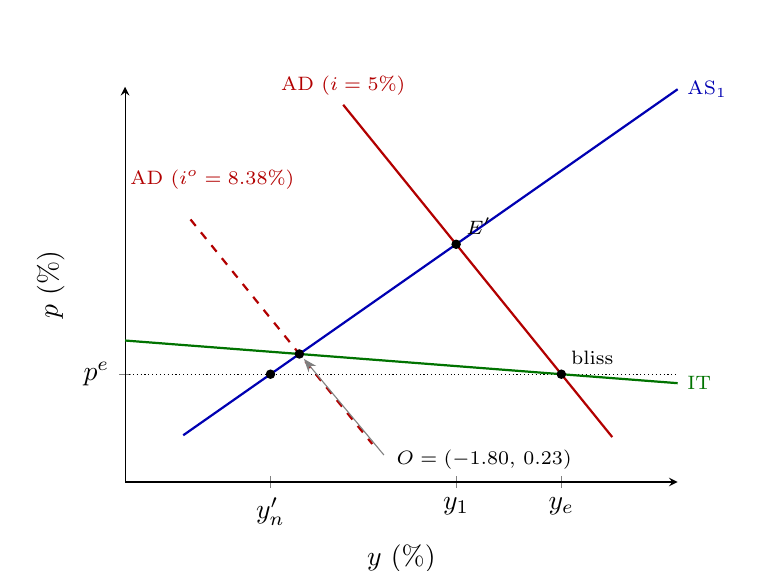
\begin{tikzpicture}
\begin{axis}[width=8.6cm,height=6.6cm,axis lines=left,xmin=-3,xmax=0.8,ymin=-1.2,ymax=3.2,clip=false,
  xlabel={$y$ (\%)},ylabel={$p$ (\%)},xtick={-2,-0.7234,0},xticklabels={$y_n'$,$y_1$,$y_e$},
  ytick={0},yticklabels={$p^e$}]
\addplot[densely dotted,domain=-3:0.8]{0};
\addplot[thick,blue!70!black,domain=-2.6:0.8]{1.1333*(x+2)};
\addplot[thick,green!45!black,domain=-3:0.8]{-x/8};
\addplot[thick,red!70!black,domain=-1.5:0.35]{-2*x};
\addplot[thick,red!70!black,dashed,domain=-2.55:-1.3]{-3.377-2*x};
\node[font=\scriptsize,blue!70!black,anchor=west] at (axis cs:0.8,3.17) {AS$_1$};
\node[font=\scriptsize,green!45!black,anchor=west] at (axis cs:0.8,-0.1) {IT};
\node[font=\scriptsize,red!70!black,anchor=south] at (axis cs:-1.5,3.0) {AD ($i=5\%$)};
\node[font=\scriptsize,red!70!black,anchor=south] at (axis cs:-2.4,1.95) {AD ($i^o=8.38\%$)};
\addplot[only marks,mark=*,mark size=1.5pt] coordinates {(-0.7234,1.4468) (-1.8013,0.2252) (0,0) (-2,0)};
\node[font=\scriptsize,anchor=south west] at (axis cs:-0.72,1.45) {$E'$};
\node[font=\scriptsize,anchor=west] at (axis cs:-1.2,-0.95) {$O=(-1.80,\,0.23)$};
\draw[-{Stealth},gray] (axis cs:-1.22,-0.9)--(axis cs:-1.77,0.17);
\node[font=\scriptsize,anchor=south west] at (axis cs:0,0) {bliss};
\end{axis}
\end{tikzpicture}\\
{\footnotesize The optimum $O$ is where AS$_1$ meets the IT line $(y-y_e)+\theta(p-p^e)=0$; the Copom raises $i$ so that AD shifts
down/left from $E'$ to $O$. AS does not move with policy.}
\end{center}
\intuicao{A mark-up shock moves $y_n$ but not $y_e$, so no rate delivers both targets. Convex losses
make the bank spread the miss; with welfare weights, relative-price dispersion is so costly
($\theta=8$) that it lets only a tenth of the shock into prices.}
\refbib{Benigno (2015), \S11, eqs.~(33)--(35), Fig.~14, pp.~521--523; \S3 on the interest-rate instrument.}
\rubrica{
\item Targeting rule by substitution: 1.5 pts.
\item $y^o=-1.80$, $p^o=+0.23$, split $1/(1+\theta\kappa)$: 1 pt (slip: $-1$ pt).
\item $i^o=8.38\%$ via $r_n=9\%$: 0.5 pt.
\item Why AS is the constraint and the money market determines $M$: 1 pt.
\item Sign relative to no policy with the condition $\theta>\sigma$: 1 pt.
\item Using AD as the constraint: max.\ 2 pts on the item. Targeting $y_n$ instead of $y_e$: max.\ 2.5 pts.
}
\gap{Lista 7 (latest content): a temporary mark-up shock moves only AS; $y-y_n$ vs $y-y_e$; why
$y_n\neq y_e$ (wedge, not stickiness); optimal policy subject to AS and why AD is not a constraint.
Lista 6, 1(d): under a rate instrument the money market determines $M$.}
\end{sol}

\ifsolucoes\else
\vfill
\begin{center}\footnotesize\textit{End of exam.}\end{center}
\fi

\end{document}
"   (run twice)
% Check fonts: pdffonts <file>.pdf  (all Type 1).
% Every number in the key: python simulado_codigo/check_simulado_02.py
% =============================================================================
\documentclass[11pt,a4paper]{article}
\usepackage[utf8]{inputenc}
\usepackage[T1]{fontenc}
\usepackage{lmodern}   % Type 1 vector fonts (replaces PK bitmaps)
\usepackage{cmap}      % ToUnicode CMap -> copyable text and accents
\usepackage[english]{babel}
\usepackage{amsmath,amssymb,amsfonts}
\usepackage[a4paper,margin=2.2cm]{geometry}
\usepackage{enumitem}
\usepackage{fancyhdr}
\usepackage{comment}
\usepackage{xcolor}
\usepackage{microtype}
\usepackage{booktabs}
\usepackage{needspace}
\usepackage{pgfplots}
\pgfplotsset{compat=1.18}
\usetikzlibrary{arrows.meta}

% ====================== CONFIGURATION ======================
\newif\ifsolucoes
\ifdefined\withsolutions\solucoestrue\else\solucoesfalse\fi

\newcommand{\disciplina}{Macroeconomics I --- MPE Insper}
\newcommand{\listatema}{Mock Final Exam 2}
\newcommand{\espacoresol}{6.5cm}

% ====================== MACHINERY ======================
\ifsolucoes\includecomment{sol}\else\excludecomment{sol}\fi

\pagestyle{fancy}\fancyhf{}
\lhead{\footnotesize\disciplina}
\rhead{\footnotesize \listatema\ifsolucoes{} --- Solutions and Rubric\fi}
\cfoot{\footnotesize\thepage}
\renewcommand{\headrulewidth}{0.3pt}
\setlength{\headheight}{14pt}

\setlist{topsep=2pt,itemsep=2pt}
\newcounter{questao}

\newcommand{\bloco}[3]{\Needspace{10\baselineskip}\bigskip\noindent
  {\large\bfseries\color{blue!55!black}Block #1 --- #2}\hfill\textit{(#3)}\par
  \noindent\rule{\linewidth}{0.3pt}\smallskip}
\newcommand{\questao}[1]{\refstepcounter{questao}\medskip\noindent
  \textbf{Question \thequestao.}~#1\par}
\newenvironment{alternativas}{\begin{enumerate}[label=\Alph*.,leftmargin=2.2em,topsep=1pt]}{\end{enumerate}}
\newcommand{\gabarito}[1]{\ifsolucoes\par\noindent\textbf{Answer:}~#1\fi}
\newcommand{\resolespaco}{\ifsolucoes\else\par\textit{Solution:}\vspace{\espacoresol}\par\fi}
\newcommand{\passo}[2]{\par\smallskip\noindent\textbf{Step #1.}~#2}
\newcommand{\intuicao}[1]{\par\smallskip\noindent\textit{Intuition.}~#1}
\newcommand{\refbib}[1]{\par\smallskip\noindent{\footnotesize\color{black!60}\textbf{Ref:} #1}}
\newcommand{\gap}[1]{\par\smallskip\noindent{\footnotesize\color{red!55!black}\textbf{Gap targeted:} #1}}
\newcommand{\trap}[1]{\par\smallskip\noindent{\small\color{red!55!black}\#~#1}}
\newcommand{\rubrica}[1]{\par\smallskip\noindent\textbf{Grading rubric.}\begin{itemize}[leftmargin=1.4em,topsep=1pt]#1\end{itemize}}

% =============================================================================
\begin{document}
\begin{center}
  {\Large\bfseries \disciplina}\\[2pt]
  {\large \listatema\ (Simulado 2) --- 2026, 3rd term}\ifsolucoes\\[2pt]\textit{Solutions and Grading Rubric}\fi
\end{center}
\vspace{2pt}

{\footnotesize\noindent\textbf{Instructions.} Four blocks of 25 points (100 in total). Duration: 3 hours,
closed book, non-programmable calculator allowed. Each block has one objective question (10 points)
and one discursive question (15 points).
\emph{Multiple choice} (items a, b): mark the single correct option; no penalty for a wrong answer.
\emph{True/False} (items c, d): the score of the T/F items is
$\max\{0,\ \text{correct}-\text{wrong}/2\}\times$ item value, i.e.\ every two wrong items cancel one
correct item; blank items do not count as wrong.
\emph{Discursive questions}: show every step; box final answers; sign every derivative before
interpreting it; label axes and curves in diagrams. Notation: Kurlat (2020) in Blocks I--III, Benigno
(2015) in Block IV. All numbers are illustrative.\par}

\ifsolucoes
\medskip
{\footnotesize\noindent\textbf{How the rubric works.} Conceptual caps (``max.\ $x$ pts'') bound an
item whatever else is right. Light penalties ($-1$ pt) apply to arithmetic slips with a correct method.
Caps and penalties are \emph{not cumulative}: when a cap applies, the penalties inside it are ignored.
Each question ends with the graded mistake it retests (``Gap targeted''). Every number below is
recomputed by \texttt{simulado\_codigo/check\_simulado\_02.py}.\par}
\fi

% =============================================================================
\bloco{I}{Measurement and national accounts}{Lecture 1 \,\textbullet\, 25 points}

\questao{(10 points) Objective items.}

\textbf{a)} (3 points) A soy chain in Mato Grosso, one year, values in R\$ million. A fertiliser
producer, which uses no intermediate inputs, sells its whole output, 30, to a soy farm. The farm
harvests soy worth 100: it sells 70 to a crushing plant and exports 30 to China. The crusher sells
soybean oil worth 150 to Brazilian households. By the production (value-added) approach, the chain's
contribution to Brazil's GDP is:
\begin{alternativas}
\item 150
\item 280
\item 180
\item 210
\item 250
\end{alternativas}
\gabarito{C.}
\begin{sol}
Value added $=(30-0)+(100-30)+(150-70)=30+70+80=\boxed{180}$. Check by expenditure:
$C+X=150+30=180$. B (280) is gross production, which counts the intermediate inputs 30 and 70 twice;
A (150) forgets the exports; D (210) subtracts only the soy input; E (250) adds the last two sales.
\refbib{Kurlat ch.~1, \S1.1 (the three approaches), pp.~15--21.}
\end{sol}

\medskip
\textbf{b)} (3 points) IBGE data for a year, in R\$ billion: GDP is 10{,}000; wages earned by
Brazilian residents on short assignments abroad, 50; profits of foreign-owned plants in Brazil sent to
their parent companies, 300; interest on Brazilian bonds held by non-residents, 150; personal transfers
sent home by Brazilians who live permanently abroad, 40. Using Kurlat's definition,
$\text{GNI}=\text{GDP}+F^{\text{out}}-F^{\text{in}}$, where $F^{\text{out}}$ is factor income earned
abroad by residents and $F^{\text{in}}$ factor income earned at home by non-residents, Brazil's GNI is:
\begin{alternativas}
\item 9{,}640
\item 10{,}400
\item 9{,}750
\item 9{,}600
\item 10{,}000
\end{alternativas}
\gabarito{D.}
\begin{sol}
$\text{GNI}=10{,}000+50-300-150=\boxed{9{,}600}$. Profits and interest are \emph{factor} income of
non-residents; the 40 are transfers, not payments to a factor of production, so they are not in GNI
(A adds them). B flips the signs; C leaves the interest out; E confuses territory (GDP) with
ownership (GNI).
\refbib{Kurlat ch.~1, \S1.1, GDP vs GNP.}
\end{sol}

\medskip
\textbf{c)} (2 points, T or F) In a year in which Brazil's gross fixed capital formation equals
17\% of GDP, Brazil's stock of fixed capital rises by 17\% of GDP.
\gabarito{F.}
\begin{sol}
Investment is a gross \emph{flow}; the stock changes by the net flow, $K_{t+1}-K_t=I_t-\delta K_t$.
With, say, $K/Y=3$ and $\delta=4\%$, $\delta K=12\%$ of GDP is replacement, and the stock rises by
only $17-12=5\%$ of GDP.
\refbib{Kurlat ch.~1, eq.~(1.2) and the depreciation discussion, p.~21.}
\end{sol}

\medskip
\textbf{d)} (2 points, T or F) In 2015 Brazil's nominal GDP grew by about 3.8\% while real GDP fell by
about 3.5\%. Hence the GDP deflator rose by less than 3.8\% that year.
\gabarito{F.}
\begin{sol}
$1+\pi_{\text{defl}}=\dfrac{1+g_{\text{nominal}}}{1+g_{\text{real}}}=\dfrac{1.038}{0.965}=1.0756$, so
$\boxed{\pi_{\text{defl}}\approx7.6\%>3.8\%}$. When real output falls, the deflator must grow
\emph{faster} than nominal GDP, not slower.
\refbib{Kurlat ch.~1, \S1.2 (real vs nominal), pp.~22--25.}
\end{sol}
\begin{sol}
\gap{Lista 1, 1(b)--(c): both lost marks were numbers that changed between the line computing them
and the line using them. Items (a) and (d) reward copying each intermediate result exactly.}
\end{sol}

% -----------------------------------------------------------------------------
\questao{(15 points) Brazil and Portugal: exchange rates, prices and welfare.
A think tank compares living standards in Brazil and Portugal with a two-good economy. Per-capita
annual quantities and local prices are:}

\begin{center}\small
\begin{tabular}{@{}lcccc@{}}
\toprule
& \multicolumn{2}{c}{Traded good $T$ (grains, manufactures)} & \multicolumn{2}{c}{Non-traded good $N$ (housing, haircuts, services)}\\
& quantity & price & quantity & price \\
\midrule
Brazil & 5 & 10 reais & 10 & 4 reais \\
Portugal & 10 & 2 euros & 15 & 2 euros \\
\bottomrule
\end{tabular}
\end{center}
\noindent The traded good obeys the law of one price at the market exchange rate. Output per worker is
$A_T=2$, $A_N=5$ in Brazil and $A_T=A_N=5$ in Portugal; within each country labour moves freely between
sectors and firms are competitive.

\textbf{a)} (5 points) Find the market exchange rate (reais per euro), Brazil's GDP per capita in
euros at the market rate and at PPP (Brazil's quantities valued at Portuguese prices), the
Brazil/Portugal ratio under each conversion, the PPP exchange rate and Brazil's price level relative
to Portugal's.
\resolespaco
\begin{sol}
\passo{1 --- market rate}{Law of one price in $T$: 10 reais $=$ 2 euros, so
$\boxed{e=5\text{ reais per euro}}$.}
\passo{2 --- nominal GDP per capita}{Brazil: $5\cdot10+10\cdot4=50+40=90$ reais. Portugal:
$10\cdot2+15\cdot2=20+30=50$ euros.}
\passo{3 --- market-rate conversion}{Brazil $=90/5=18$ euros; ratio $18/50=\boxed{0.36}$.}
\passo{4 --- PPP conversion}{Brazil at Portuguese prices: $5\cdot2+10\cdot2=10+20=30$ euros; ratio
$30/50=\boxed{0.60}$.}
\passo{5 --- PPP rate and price level}{$e^{\text{PPP}}=90/30=\boxed{3\text{ reais per euro}}$.
Relative price level $=e^{\text{PPP}}/e=3/5=\boxed{0.6}$: Brazil's basket costs 60\% of what it costs in
Portugal.}
\passo{6 --- check}{$0.60/0.36=1.667=1/0.6$: the two ratios differ exactly by the price level.}
\refbib{Kurlat ch.~1, \S1.2, international comparisons and PPP, pp.~25--27.}
\rubrica{
\item $e=5$: 1 pt. Market-rate ratio 0.36: 1 pt. PPP ratio 0.60: 1.5 pts. $e^{\text{PPP}}=3$ and price level 0.6: 1.5 pts.
\item Valuing Portugal at Brazilian prices instead is a legitimate PPP (ratio $90/(10\cdot10+15\cdot4)=0.5625$) if stated: full marks for that part; unstated mix of bases: max.\ 3 pts.
\item Arithmetic slip with correct method: $-1$ pt.
}
\end{sol}

\textbf{b)} (5 points) Which good drives the gap between the two ratios? Derive the relative price of
the non-traded good in each country from the firms' and workers' conditions, explain the direction of
the bias of the market-rate comparison (Balassa--Samuelson), and explain why ``transport and trade
costs'' is \emph{not} the explanation here.
\resolespaco
\begin{sol}
\passo{1 --- split Brazil's output by good}{Traded: $50/5=10$ euros at the market rate and
$5\cdot2=10$ euros at PPP --- identical. Non-traded: $40/5=8$ euros at the market rate and
$10\cdot2=20$ euros at PPP. \boxed{\text{The whole 12-euro gap comes from the non-traded good.}}}
\passo{2 --- wage equalisation}{Competitive firms pay the value of the marginal product and workers
move until wages are equal: $W=p_TA_T=p_NA_N\;\Rightarrow\;\boxed{p_N/p_T=A_T/A_N}$.
Brazil: $2/5=0.4=4/10$ \checkmark. Portugal: $5/5=1=2/2$ \checkmark.}
\passo{3 --- mechanism}{$A_T^{BR}/A_T^{PT}=0.4$ while $A_N^{BR}/A_N^{PT}=1$: Brazil's productivity gap
is in traded goods.
$A_T\downarrow\;\rightarrow\;W=p_TA_T\downarrow$ (with $p_T$ tied to the world price)
$\rightarrow\;p_N=W/A_N\downarrow\;\rightarrow$ non-traded goods are cheap in Brazil
$\rightarrow$ the market rate values Brazil's non-traded output at a price nobody pays in Portugal.}
\passo{4 --- direction}{\boxed{\text{The market rate understates Brazil's real output}} (0.36 vs 0.60),
and more so the larger the productivity gap in $T$ relative to $N$. A uniform gap in both sectors
would leave $A_T/A_N$ and hence the price level unchanged.}
\passo{5 --- why not trade costs}{Trade costs are frictions on \emph{traded} goods, and in this
economy the law of one price holds exactly for $T$ --- where the market rate works perfectly (Step 1).
The bias sits in the good that is never traded, for which there is no arbitrage at \emph{any} trade
cost. Trade costs would also push the importer's price up, not produce a systematic ``poorer is
cheaper'' pattern.}
\intuicao{Wages are set by productivity in the sector that faces world prices, and the same wage is
paid to haircutters whose productivity is the same everywhere. Cheap services in poor countries are a
wage fact, not a transport fact.}
\refbib{Kurlat ch.~1, \S1.2, pp.~25--27; Balassa--Samuelson as derived in the course notes
(\texttt{Map/aula-01-mensuracao/04}).}
\rubrica{
\item Decomposition showing the gap is entirely in $N$: 1.5 pts.
\item $p_N/p_T=A_T/A_N$ from wage equalisation, both countries checked: 1.5 pts.
\item Direction (understates) with the mechanism in words: 1 pt.
\item Why trade costs fail: 1 pt.
\item Explaining the gap by trade/import costs: max.\ 2 pts on the item (conceptual cap).
}
\end{sol}

\textbf{c)} (5 points) Welfare beyond GDP. Use Kurlat's consumption-equivalent (Jones--Klenow)
measure with log utility ($\sigma=1$), lognormal consumption within each country and equal leisure
(set the leisure term to zero). A person lives in a country with probability $e=\text{LE}/100$ and then
enjoys $\bar u+\mathbb E[\ln c]$. Data: Brazil's mean consumption per capita is 60\% of Portugal's
(normalise Portugal's to 1); the standard deviation of log consumption is $s_{BR}=0.9$ and
$s_{PT}=0.5$; life expectancy is 76 and 81 years; $\bar u=5$. Find $\lambda$, the factor applied to
Portuguese consumption that makes a person behind the veil indifferent between the two countries,
decompose $\ln\lambda$ into consumption, inequality and life-expectancy terms, and compare with (a).
\resolespaco
\begin{sol}
\passo{1 --- set-up}{Indifference:
$e_{PT}\left[\bar u+\ln\lambda+\mathbb E\ln c_{PT}\right]=e_{BR}\left[\bar u+\mathbb E\ln c_{BR}\right]$.
Lognormal: $\mathbb E\ln c=\ln\bar c-\tfrac12s^2$.}
\passo{2 --- ingredients}{$\mathbb E\ln c_{PT}=0-\tfrac12(0.25)=-0.125$;
$\mathbb E\ln c_{BR}=\ln0.6-\tfrac12(0.81)=-0.5108-0.405=-0.9158$.
Flow values: $v_{PT}=5-0.125=4.875$, $v_{BR}=5-0.9158=4.0842$.}
\passo{3 --- solve}{$\ln\lambda=\dfrac{e_{BR}}{e_{PT}}v_{BR}-v_{PT}=\dfrac{76}{81}(4.0842)-4.875
=0.93827\cdot4.0842-4.875=3.8321-4.875=\boxed{-1.043}$, so $\boxed{\lambda=e^{-1.043}\approx0.35}$.}
\passo{4 --- decomposition}{$\ln\lambda=\underbrace{\ln0.6}_{\text{consumption}}
\underbrace{-\tfrac12(0.81-0.25)}_{\text{inequality}}
+\underbrace{\left(\tfrac{76}{81}-1\right)4.0842}_{\text{life expectancy}}
=-0.511-0.280-0.252=-1.043$ \checkmark\ (exact, not an approximation).}
\passo{5 --- comparison}{The PPP ratio 0.60 is the right GDP benchmark; welfare is lower, 0.35,
because inequality and shorter lives add $0.53$ log points to the gap. That 0.35 is close to the
market-rate ratio 0.36 is a coincidence: the market rate is wrong for a price reason (b); $\lambda$ is
low for inequality and mortality reasons.}
\intuicao{Behind the veil, inequality is risk, and log utility prices it at half the log variance;
a shorter life scales down every year's utility, weighted by the value of being alive, $\bar u$.}
\refbib{Kurlat ch.~2, \S2.2 (Jones--Klenow), eqs.~(2.2.1)--(2.2.3), pp.~33--41.}
\rubrica{
\item Indifference condition written with $e$ multiplying the whole bracket: 1.5 pts.
\item $\mathbb E\ln c=\ln\bar c-s^2/2$ used for both countries: 1 pt.
\item $\ln\lambda=-1.043$, $\lambda\approx0.35$: 1 pt; three terms: 1 pt.
\item Comparison with 0.60 (not 0.36) as the benchmark: 0.5 pt.
\item Treating life expectancy additively (not as a probability weight): max.\ 2.5 pts.
\item Reading $\lambda\approx0.36$ as vindicating the market rate: $-1$ pt.
}
\gap{Lista 1, 1(e): the PPP gap was explained with import/export costs; the mark is for
non-tradables and Balassa--Samuelson. Also Lista 1's rule ``answer every object'': (a) asks for five
numbers.}
\end{sol}

% =============================================================================
\bloco{II}{Long-run growth and the Solow model}{Lectures 2--3 \,\textbullet\, 25 points}

\questao{(10 points) Objective items.}

\textbf{a)} (3 points) Solow model in \emph{per-worker} terms, no technological progress,
$Y=K^{1/3}L^{2/3}$, $s=0.20$, $\delta=0.05$. Starting from its steady state, Brazil's population growth
falls permanently from 2\% to 1\% a year (the demographic transition). Which statement about
steady-state output per worker $y^\ast$, the growth of $y$ during the transition and the growth of
aggregate $Y$ in the new steady state is correct?
\begin{alternativas}
\item $y^\ast$ rises by about 26.0\%; $g_y>0$ only during the transition; $g_Y$ falls from 2\% to 1\%.
\item $y^\ast$ rises by about 8.0\%; $g_y>0$ only during the transition; $g_Y$ stays at 2\%.
\item $y^\ast$ rises by about 8.0\%; $g_y$ is permanently higher than before; $g_Y$ stays at 2\%.
\item $y^\ast$ rises by about 16.7\%; $g_y>0$ only during the transition; $g_Y$ falls from 2\% to 1\%.
\item $y^\ast$ rises by about 8.0\%; $g_y>0$ only during the transition; $g_Y$ falls from 2\% to 1\%.
\end{alternativas}
\gabarito{E.}
\begin{sol}
$k^\ast=\left(\dfrac{s}{n+\delta}\right)^{\frac{1}{1-\alpha}}$, $y^\ast=\left(\dfrac{s}{n+\delta}\right)^{\frac{\alpha}{1-\alpha}}
=\left(\dfrac{s}{n+\delta}\right)^{1/2}$, so
$\dfrac{y^\ast_{new}}{y^\ast_{old}}=\left(\dfrac{0.07}{0.06}\right)^{1/2}=1.080$: $\boxed{+8.0\%}$.
The flatter break-even line $(n'+\delta)k$ leaves $sf(k)>(n'+\delta)k$ at the old $k^\ast$, so $k$ and
$y$ grow until the new steady state and then $g_y=0$ again. Aggregate $Y=yL$ grows at $g_y+n$: $n$
before, $n'$ after. \#~Higher level, same (zero) steady-state per-worker growth, higher growth during
convergence, \emph{lower} aggregate growth. A uses $k^\ast$ ($+26.0\%$); D uses the ratio of
break-even slopes ($+16.7\%$); B and C forget aggregate vs per worker.
\end{sol}
\begin{sol}
\begin{center}
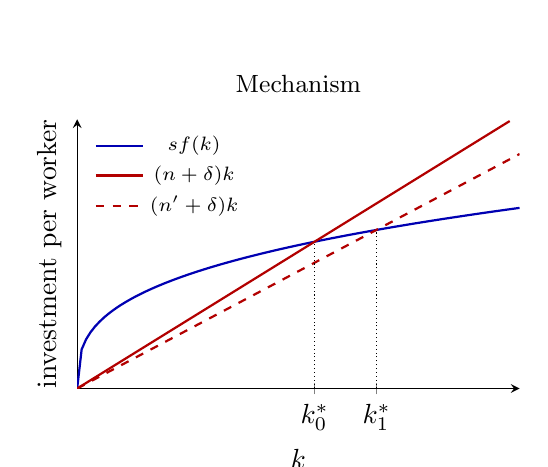
\begin{tikzpicture}
\begin{axis}[width=7.2cm,height=5cm,axis lines=left,xmin=0,xmax=9,ymin=0,ymax=0.62,
  xlabel={$k$},ylabel={investment per worker},xtick={4.83,6.09},xticklabels={$k^\ast_0$,$k^\ast_1$},
  ytick=\empty,title={\small Mechanism},legend style={font=\scriptsize,at={(0.02,0.98)},anchor=north west,draw=none}]
\addplot[thick,blue!70!black,domain=0:9,samples=100]{0.2*x^(1/3)};
\addplot[thick,red!70!black,domain=0:8.8]{0.07*x};
\addplot[thick,red!70!black,dashed,domain=0:9]{0.06*x};
\legend{$sf(k)$,$(n+\delta)k$,$(n'+\delta)k$}
\draw[densely dotted] (axis cs:4.83,0)--(axis cs:4.83,0.338);
\draw[densely dotted] (axis cs:6.09,0)--(axis cs:6.09,0.365);
\end{axis}
\end{tikzpicture}\quad
\begin{tikzpicture}
\begin{axis}[width=7.2cm,height=5cm,axis lines=left,xmin=-10,xmax=60,ymin=0.5,ymax=0.63,
  xlabel={time},ylabel={$\ln y$},xtick={0},xticklabels={$t_0$},ytick={0.525,0.602},
  yticklabels={$\ln y^\ast_0$,$\ln y^\ast_1$},title={\small Time path}]
\addplot[thick,blue!70!black,domain=-10:0]{0.5249};
\addplot[thick,blue!70!black,domain=0:60,samples=60]{0.6019-(0.6019-0.5249)*exp(-0.04*x)};
\addplot[densely dotted,domain=-10:60]{0.6019};
\end{axis}
\end{tikzpicture}
\end{center}
{\footnotesize Left: $n$ falls, the break-even ray rotates down, $k^\ast$ rises. Right: $\ln y$ rises
during the transition and flattens; $\ln Y$ (not drawn) has slope $n=2\%$ before and $n'=1\%$ after.}
\refbib{Kurlat ch.~4, \S4.2 (comparative statics), pp.~59--61.}
\end{sol}

\medskip
\textbf{b)} (3 points) Same model with $\alpha=0.35$ and $n+\delta=0.07$; Brazil saves 17\% of GDP.
Which statement is correct about the golden-rule saving rate and the effect on steady-state
consumption per worker of raising $s$ from 0.17 to 0.25?
\begin{alternativas}
\item $s_{GR}=0.65$; raising $s$ from 0.17 to 0.25 lowers steady-state consumption per worker.
\item $s_{GR}=0.35$; raising $s$ from 0.17 to 0.25 raises steady-state consumption per worker.
\item $s_{GR}=0.35$; raising $s$ from 0.17 to 0.25 lowers steady-state consumption per worker.
\item $s_{GR}=1.00$; raising $s$ from 0.17 to 0.25 raises steady-state consumption per worker.
\end{alternativas}
\gabarito{B.}
\begin{sol}
$c^\ast=f(k^\ast)-(n+\delta)k^\ast$ is maximised at $f'(k_{GR})=n+\delta$; with Cobb--Douglas
$\alpha k^{\alpha-1}=n+\delta$ and $s\,k^{\alpha-1}=n+\delta$ give $\boxed{s_{GR}=\alpha=0.35}$.
$c^\ast(s)=(1-s)\left(\frac{s}{0.07}\right)^{0.35/0.65}$: $c^\ast(0.17)=1.338<c^\ast(0.25)=1.488$.
Below the golden rule a higher $s$ raises long-run consumption (after an initial fall). A uses
$1-\alpha$; C reads only the $(1-s)$ factor; D maximises $k^\ast$, not $c^\ast$.
\refbib{Kurlat ch.~4, \S4.3 (golden rule), pp.~61--63.}
\end{sol}

\medskip
\textbf{c)} (2 points, T or F) Of two economies with the same technology, depreciation and population
growth, the one with lower capital per worker necessarily grows faster.
\gabarito{F.}
\begin{sol}
Convergence is \emph{conditional}: $g_k=s\,k^{\alpha-1}-(n+\delta)$ depends on the distance to each
economy's own steady state, which depends on $s$. With $\alpha=1/3$, $n+\delta=0.07$: $X$ with $k=3$,
$s=0.10$ has $g_k=-2.2\%$; $Z$ with $k=5$, $s=0.30$ has $g_k=+3.3\%$.
\refbib{Kurlat ch.~5, \S5.1--\S5.3 (convergence), pp.~75--86.}
\end{sol}

\medskip
\textbf{d)} (2 points, T or F) If a country's national accounts show a capital share of income of one
third, the same as in undistorted economies with $\alpha=1/3$, then its measured TFP reflects only
technology.
\gabarito{F.}
\begin{sol}
Normal factor shares do not rule out distortions. A requirement to hold unproductive capital recorded
as capital leaves $rK/Y=\alpha$ exactly and puts the whole distortion in the residual,
$\hat A=A(1+\theta)^{-\alpha}$ (Question 4).
\refbib{Kurlat ch.~5, \S5.4--\S5.5 (growth and development accounting), pp.~86--95.}
\gap{Lista 1, 4(b): a Solow comparative static in $n$ left blank; Lista 1, 4(a): aggregate vs per
capita (item a). Item (d) previews Lista 2, 2(c).}
\end{sol}

% -----------------------------------------------------------------------------
\questao{(15 points) ``Custo Brasil'' in the growth accounts.
Output is $Y=AK_P^{\alpha}L^{1-\alpha}$ with $\alpha=0.4$, where $K_P$ is productive capital.
Regulation, legal uncertainty and crime force every firm to hold $\theta$ units of \emph{compliance
capital} (duplicate tax-filing systems, armoured vehicles, walls, back-up generators) for each unit of
productive capital. Compliance capital produces nothing, but the national accounts record it as capital
like any other, so measured capital is $K=K_P+\theta K_P$. Capital is rented at $r$ and labour hired
at $w$ in competitive markets. Today $\theta=0.6$.}

\textbf{a)} (5 points) Write aggregate output as a function of $A,K,L,\theta$. What share of measured
capital is unproductive? How much output is lost relative to an economy with $\theta=0$ and the same
$A,K,L$? State the base of your percentage.
\resolespaco
\begin{sol}
\passo{1 --- composition}{$K=(1+\theta)K_P\Rightarrow K_P=K/(1+\theta)$.}
\passo{2 --- output}{$Y=A\left(\dfrac{K}{1+\theta}\right)^{\alpha}L^{1-\alpha}
\;\Rightarrow\;\boxed{Y=\underbrace{A(1+\theta)^{-\alpha}}_{\text{wedge on TFP}}K^{\alpha}L^{1-\alpha}}$.}
\passo{3 --- unproductive share}{$\dfrac{\theta K_P}{(1+\theta)K_P}=\dfrac{0.6}{1.6}=\boxed{37.5\%}$.}
\passo{4 --- output lost}{$\dfrac{Y(\theta)}{Y(0)}=(1.6)^{-0.4}=e^{-0.4\ln1.6}=e^{-0.4\cdot0.4700}=e^{-0.1880}=0.8286$.
\boxed{\text{Output is }17.1\%\text{ below the undistorted level}} (base: $Y(0)$). Equivalently,
removing $\theta$ would raise output by $1/0.8286-1=\boxed{20.7\%}$ (base: $Y(\theta)$).
\#~Careful with the chosen base.}
\intuicao{A third of the capital stock does no work, but output falls by less than a third because
capital has diminishing returns and a share of only 0.4.}
\refbib{Kurlat ch.~5, \S5.4--\S5.5, pp.~86--95.}
\rubrica{
\item $K_P=K/(1+\theta)$ and the boxed $Y$ with the wedge named: 2 pts.
\item Share 37.5\%: 1 pt.
\item Loss 17.1\% (or gain 20.7\%) with the base stated: 2 pts; no base stated: $-1$ pt.
\item Loss computed as $\theta/(1+\theta)=37.5\%$ of output: max.\ 2 pts on the item.
}
\end{sol}

\textbf{b)} (5 points) Write the representative firm's problem and first-order conditions and derive
the measured factor shares $rK/Y$ and $wL/Y$. A development accountant has data on $Y$, $K$, $L$ and
factor payments only. What does she conclude about $\alpha$ and about TFP? Who bears the cost of
$\theta$?
\resolespaco
\begin{sol}
\passo{1 --- problem}{To use $K_P$ productive units the firm must rent $(1+\theta)K_P$:
$\max_{K_P,L}\;AK_P^{\alpha}L^{1-\alpha}-r(1+\theta)K_P-wL$.}
\passo{2 --- FOCs}{$\alpha\dfrac{Y}{K_P}=r(1+\theta)$ and $(1-\alpha)\dfrac{Y}{L}=w$.}
\passo{3 --- shares}{Using $(1+\theta)K_P=K$: $r=\dfrac{\alpha Y}{(1+\theta)K_P}=\alpha\dfrac{Y}{K}$, so
$\boxed{rK/Y=\alpha=0.4}$ and $\boxed{wL/Y=1-\alpha=0.6}$: \emph{undistorted}.}
\passo{4 --- the accountant}{She sets $\hat\alpha=rK/Y=0.4=\alpha$ (correct) and computes
$\hat A=\dfrac{Y}{K^{\hat\alpha}L^{1-\hat\alpha}}=\boxed{A(1+\theta)^{-\alpha}=0.83A}$.
She concludes that Brazil has 17\% lower \emph{technology}. Wrong: technology is $A$; the gap is a
wasted-capital distortion that the data classify as productivity.}
\passo{5 --- incidence}{The rental rate $r=\alpha Y/K$ and the wage
$w=(1-\alpha)\hat A(K/L)^{\alpha}$ are both lower at given $K/L$ by the factor $(1+\theta)^{-\alpha}$.
\#~Workers are also affected: capital and labour are complements.}
\intuicao{Each productive machine drags $\theta$ idle ones with it, so capital looks less productive
by exactly the amount it is paid less: the share is untouched, the level is not.}
\refbib{Kurlat ch.~5, \S5.4 (factor shares and TFP), pp.~86--92.}
\rubrica{
\item Problem with cost $r(1+\theta)K_P$ and both FOCs: 1.5 pts.
\item $rK/Y=\alpha$, $wL/Y=1-\alpha$: 1.5 pts.
\item $\hat\alpha=\alpha$ and $\hat A=A(1+\theta)^{-\alpha}$, read as distortion, not technology: 1.5 pts.
\item Workers also bear the cost: 0.5 pt.
\item Claiming the capital share is distorted ($\hat\alpha\neq\alpha$): max.\ 2 pts on the item.
}
\end{sol}

\textbf{c)} (5 points) A reform (tax simplification, digital filing, lower crime) cuts $\theta$ from
0.6 to 0.28 gradually over the decade 2027--2036, while true $A$ stays constant; $K$ and $L$ grow at
whatever rates they grow. Write the growth-accounting decomposition, compute the average annual Solow
residual, say what it would show if $\theta$ instead \emph{rose} from 0.28 to 0.6, and explain why
this is consistent with Kurlat's reading of the residual.
\resolespaco
\begin{sol}
\passo{1 --- decomposition}{From $Y_t=A(1+\theta_t)^{-\alpha}K_t^{\alpha}L_t^{1-\alpha}$, in logs over the decade:
$\Delta\ln Y=\alpha\,\Delta\ln K+(1-\alpha)\Delta\ln L+\underbrace{\Delta\ln A}_{=0}\underbrace{-\alpha\,\Delta\ln(1+\theta)}_{\Delta\theta}$.
The accountant computes $\text{residual}=\Delta\ln Y-\alpha\Delta\ln K-(1-\alpha)\Delta\ln L=\underbrace{g_{\text{TFP}}+\Delta\theta\text{ term}}_{\text{Solow residual}}$.}
\passo{2 --- number}{$\alpha\ln\dfrac{1+\theta}{1+\theta'}=0.4\ln\dfrac{1.6}{1.28}=0.4\ln1.25=0.4\cdot0.2231=0.0893$
over ten years, i.e.\ $\boxed{\approx0.89\text{ pp per year}}$ of measured ``TFP growth'' with zero
technical progress. $\ln\hat A$ goes from $-0.188$ to $-0.099$.}
\passo{3 --- the reverse}{If $\theta$ rose from 0.28 to 0.6 the residual would be
$\boxed{-0.89\text{ pp per year}}$: measured technological regress with unchanged technology.}
\passo{4 --- check}{$K$ and $L$ are subtracted with the right weights (shares are undistorted, (b)),
so the $\theta$ effect lands entirely in the residual whatever $K$ and $L$ do.}
\passo{5 --- Kurlat's reading}{The residual is whatever output growth the measured inputs do not
explain --- ``a measure of our ignorance''. It contains technology \emph{and} the efficiency with which
measured inputs are used (regulation, institutions, misallocation). A falling $\theta$ is exactly an
efficiency gain in the use of measured capital, so it belongs in the residual.}
\begin{center}
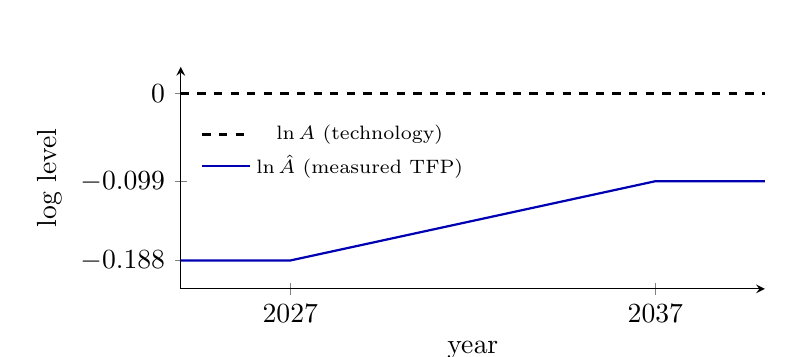
\begin{tikzpicture}
\begin{axis}[width=9cm,height=4.4cm,axis lines=left,xmin=2024,xmax=2040,ymin=-0.22,ymax=0.03,
  xlabel={year},ylabel={log level},xtick={2027,2037},xticklabels={2027,2037},
  ytick={-0.188,-0.099,0},yticklabels={$-0.188$,$-0.099$,$0$},
  legend style={font=\scriptsize,at={(0.02,0.62)},anchor=west,draw=none},
  x tick label style={/pgf/number format/1000 sep=}]
\addplot[thick,dashed,black,domain=2024:2040]{0};
\addplot[thick,blue!70!black] coordinates {(2024,-0.188) (2027,-0.188) (2037,-0.0987) (2040,-0.0987)};
\legend{$\ln A$ (technology),$\ln\hat A$ (measured TFP)}
\end{axis}
\end{tikzpicture}\\
{\footnotesize Measured TFP rises 0.89 pp a year during the reform and stops when $\theta$ stops falling; true $A$ never moves.}
\end{center}
\intuicao{The reform does not invent anything; it releases capital that was already paid for. The
data see more output from the same measured inputs and call it productivity.}
\refbib{Kurlat ch.~5, \S5.4--\S5.5 (growth accounting and what the residual contains), pp.~86--95.}
\rubrica{
\item Decomposition with the residual split into $g_{\text{TFP}}$ and the $\theta$ term: 1.5 pts.
\item $0.4\ln1.25=0.089$, about 0.89 pp per year: 1.5 pts (arithmetic slip: $-1$ pt).
\item Reverse case with the sign: 1 pt.
\item Kurlat's reading of the residual: 1 pt.
\item Residual set to zero ``because $A$ is constant'': max.\ 1 pt on the item.
}
\gap{Lista 2, 2(d), left blank: the growth-accounting residual when a capital-wasting distortion
falls. Items (a)--(c) of Lista 2 were right; this question re-asks (d) with new numbers.}
\end{sol}

% =============================================================================
\bloco{III}{Microfoundations: consumption, labour and general equilibrium}{Lectures 4--6 \,\textbullet\, 25 points}

\questao{(10 points) Objective items.}

\textbf{a)} (3 points) A two-period household (Kurlat ch.~6) has $u=\ln c_1+\beta\ln c_2$ with
$\beta=1$, faces $r=0$, can borrow and lend freely and earns $y_1=y_2=10{,}000$ reais. Consider three
separate scenarios, each against this baseline: (i) a one-off bonus of 1{,}000 today (an extraordinary
FGTS withdrawal); (ii) a credible announcement today of a raise of 1{,}000 paid in period 2 only;
(iii) a permanent raise of 1{,}000 in both periods. The changes in $c_1$ in (i), (ii), (iii) are:
\begin{alternativas}
\item 1{,}000; \ 0; \ 1{,}000
\item 500; \ 0; \ 1{,}000
\item 500; \ 500; \ 1{,}000
\item 500; \ 500; \ 500
\item 1{,}000; \ 500; \ 2{,}000
\end{alternativas}
\gabarito{C.}
\begin{sol}
With log utility $c_1=\dfrac{y_1+y_2/(1+r)}{1+\beta}=\dfrac{y_1+y_2}{2}$. (i) $\Delta W=1{,}000\Rightarrow\Delta c_1=500$;
(ii) $\Delta W=1{,}000/(1+0)=1{,}000\Rightarrow\Delta c_1=500$: news about future income moves
consumption \emph{today}, financed by borrowing; (iii) $\Delta W=2{,}000\Rightarrow\Delta c_1=1{,}000$.
\boxed{500;\ 500;\ 1{,}000}. A is Keynesian (current income only); B ignores the news.
\refbib{Kurlat ch.~6, \S6.2--\S6.3 (permanent income), pp.~105--120.}
\end{sol}

\medskip
\textbf{b)} (3 points) The government must raise a given revenue from households that save. It can tax
interest income or levy a lump-sum tax in period 2 that raises the same revenue. With CRRA utility,
which statement is correct?
\begin{alternativas}
\item Only the tax on interest changes $c_2/c_1$, through the net return in the Euler equation; at equal revenue the lump sum gives higher utility.
\item Both taxes lower $c_2/c_1$ by the same amount, because they raise the same revenue in present value and so lower wealth equally.
\item Only the lump-sum tax changes $c_2/c_1$, because it lowers wealth; the tax on interest is neutral once its revenue is fixed.
\item Only the tax on interest changes $c_2/c_1$, through the net return in the Euler equation; at equal revenue both give the same utility.
\end{alternativas}
\gabarito{A.}
\begin{sol}
Euler: $u'(c_1)=\beta[1+r(1-\tau)]u'(c_2)\Rightarrow c_2/c_1=\{\beta[1+r(1-\tau)]\}^{1/\sigma}$: the
\emph{intertemporal margin} is distorted. The lump sum shifts the budget line in parallel and leaves
$c_2/c_1=[\beta(1+r)]^{1/\sigma}$. At equal revenue $T=\tau ra$, the plan chosen under the interest tax
costs exactly $y_1+(y_2-T)/(1+r)$ at market prices, so it was affordable under the lump sum and not
chosen: \boxed{U^{\text{lump sum}}>U^{\text{interest tax}}}, the difference being deadweight loss
(D misses this).
\refbib{Kurlat ch.~6, \S6.2--\S6.4 (taxes in the two-period model), pp.~105--126.}
\end{sol}

\medskip
\textbf{c)} (2 points, T or F) A household with $u=\ln c_1+\beta\ln c_2$ earns $y_1>0$ in period 1 and
nothing in period 2 (no taxes), so it is a net saver. When $r$ rises it raises $c_1$, because for a
saver the income effect of a higher return dominates the substitution effect.
\gabarito{F.}
\begin{sol}
$c_1=\dfrac{y_1}{1+\beta}$, independent of $r$: with $\sigma=1$ and no future income to revalue, the
income and substitution effects cancel \emph{exactly}. The sign of $\partial c_1/\partial r$ is that
of $\sigma-1$; the income effect wins only if $\sigma>1$.
\refbib{Kurlat ch.~6, \S6.2 (the effect of interest rates), pp.~108--115.}
\end{sol}

\medskip
\textbf{d)} (2 points, T or F) With $u=\ln c-\chi\,h^{1+\eta}/(1+\eta)$ and no non-labour income, hours
do not respond to a permanent change in the wage (the Marshallian elasticity is zero). Therefore a
temporary, anticipated wage rise within a life of given wealth leaves hours unchanged too: the Frisch
elasticity is also zero.
\gabarito{F.}
\begin{sol}
Marshallian: $\chi h^{\eta}=w/c=w/(wh)=1/h$, hours constant. Frisch (marginal utility of wealth
$\mu$ fixed): $\chi h^{\eta}=\mu w\Rightarrow\varepsilon^F=1/\eta>0$. The ordering is
$\varepsilon^F\ge\varepsilon^H\ge\varepsilon^M$; a zero Marshallian elasticity means two effects
cancel, not that labour supply is unresponsive.
\refbib{Kurlat ch.~7, \S7.3--\S7.4, pp.~137--142.}
\gap{Lista 3, 1(b): no permanent-income story for a rise in expected $y_2$ (item a). Lista 3, 2(d): the
equal-revenue lump-sum comparison and the distorted margin were never stated (item b).}
\end{sol}

% -----------------------------------------------------------------------------
\questao{(15 points) An agribusiness productivity boom in general equilibrium.
A one-period economy has a fixed capital stock $\bar K$. The representative household owns $\bar K$ and
the firm, has one unit of time and utility $u=\dfrac{c^{1-\sigma}}{1-\sigma}+\psi\ln(1-L)$ with
$\psi=2/3$ ($\sigma$ is the curvature of utility; $1/\sigma$ the elasticity of substitution).
The competitive firm produces $Y=A\bar K^{\alpha}L^{1-\alpha}$ with $\alpha=1/3$. At the baseline
$A\bar K^{\alpha}=2^{2/3}$ and $\sigma=2$. New seed varieties raise $A$ in agriculture, which we treat
as a rise in aggregate $A$.}

\textbf{a)} (5 points) Write the household's and the firm's problems, the first-order conditions and the
market-clearing conditions. Show that profits are zero. Reduce the equilibrium to one equation in $L$,
verify that $L=1/2$ at the baseline, and compute $c$, $w$ and $r^K\bar K$.
\resolespaco
\begin{sol}
\passo{1 --- household}{$\max_{c,L}\ \frac{c^{1-\sigma}}{1-\sigma}+\psi\ln(1-L)$ s.t.\
$c=wL+r^K\bar K+\Pi$. FOC: $\boxed{\dfrac{\psi}{1-L}=w\,c^{-\sigma}}$ (MRS between leisure and
consumption $=$ real wage).}
\passo{2 --- firm}{$\max_L\ A\bar K^{\alpha}L^{1-\alpha}-wL-r^K\bar K$:
$w=(1-\alpha)\dfrac{Y}{L}$ (MPL), $r^K=\alpha\dfrac{Y}{\bar K}$ (MPK).
$\Pi=Y-(1-\alpha)Y-\alpha Y=0$ (constant returns, Euler's theorem).}
\passo{3 --- clearing}{Goods: $c=Y$ (no investment, no government). Capital: supply fixed at $\bar K$.}
\passo{4 --- one equation}{Let $\tilde A=A\bar K^{\alpha}$, so $c=\tilde AL^{1-\alpha}$ and
$w=(1-\alpha)\tilde AL^{-\alpha}$. Substituting into Step 1:
$\boxed{\psi\dfrac{L^{\alpha+(1-\alpha)\sigma}}{1-L}=(1-\alpha)\tilde A^{1-\sigma}}$ (MRS $=$ MPL).
The left side rises in $L$, so the solution is unique.}
\passo{5 --- verify}{$\sigma=2$: exponent $\tfrac13+\tfrac43=\tfrac53$. LHS at $L=\tfrac12$:
$\tfrac23\cdot\dfrac{2^{-5/3}}{2^{-1}}=\tfrac23\,2^{-2/3}$. RHS: $\tfrac23(2^{2/3})^{-1}=\tfrac23\,2^{-2/3}$ \checkmark.
Then $\boxed{c=Y=2^{2/3}\,2^{-2/3}=1}$, $\boxed{w=\tfrac23\cdot1/\tfrac12=\tfrac43}$,
$\boxed{r^K\bar K=\tfrac13}$; check $wL+r^K\bar K=\tfrac23+\tfrac13=1=Y$.}
\refbib{Kurlat ch.~9, \S9.1--\S9.2 (competitive equilibrium), pp.~165--180; ch.~7, \S7.2.}
\rubrica{
\item Both problems and FOCs, including MRS $=w$: 2 pts.
\item Zero profits and $c=Y$: 1 pt.
\item Equation in $L$ and the baseline check with $c,w,r^K\bar K$: 2 pts.
\item Adding the principal $\bar K$ to household income: $-1$ pt (budget no longer matches $c=Y$).
}
\end{sol}

\textbf{b)} (5 points) Derive $d\ln L/d\ln A$ in general and sign it by $\sigma$. Evaluate it at the
baseline and give the first-order effects of a 10\% rise in $A$ on $L$, $w$, $r^K$ and $c$. Explain in
words that match the sign.
\resolespaco
\begin{sol}
\passo{1 --- differentiate}{Log of the equation in (a):
$\ln\psi+[\alpha+(1-\alpha)\sigma]\ln L-\ln(1-L)=\ln(1-\alpha)+(1-\sigma)\ln\tilde A$.
Differentiating, with $d\ln\tilde A=d\ln A$:
$\boxed{\dfrac{d\ln L}{d\ln A}=\dfrac{1-\sigma}{\alpha+(1-\alpha)\sigma+\frac{L}{1-L}}}$.}
\passo{2 --- sign}{The denominator is positive, so the sign is that of $1-\sigma$:
$\sigma<1\Rightarrow L\uparrow$; $\sigma=1\Rightarrow L$ unchanged; $\sigma>1\Rightarrow L\downarrow$.}
\passo{3 --- baseline}{$\sigma=2$, $L=\tfrac12$: $\dfrac{-1}{\frac13+\frac43+1}=\dfrac{-1}{8/3}=\boxed{-0.375}$.}
\passo{4 --- 10\% boom}{$d\ln L=-3.75\%$. $d\ln w=d\ln A-\alpha\,d\ln L=10+\tfrac13(3.75)=\boxed{+11.25\%}$.
$d\ln r^K=d\ln A+(1-\alpha)d\ln L=10-\tfrac23(3.75)=\boxed{+7.5\%}$.
$d\ln c=d\ln Y=d\ln A+(1-\alpha)d\ln L=\boxed{+7.5\%}$.}
\passo{5 --- words}{$A\uparrow\rightarrow w\uparrow$: leisure is dearer (substitution effect, work more)
but the household is richer (income effect, enjoy more leisure). With $\sigma=2$ marginal utility of
consumption falls fast as $c$ rises, so the \emph{income effect dominates} and hours fall. Output and
consumption still rise, by less than $A$.}
\intuicao{$\sigma$ measures how fast extra consumption loses value. Above one, a richer household
prefers to take part of its gain as leisure; at exactly one the two effects cancel.}
\refbib{Kurlat ch.~7, \S7.2 (income and substitution effects), pp.~131--137; ch.~9, \S9.2.}
\rubrica{
\item Correct derivative: 2 pts. Sign by $\sigma$ with the three cases: 1 pt.
\item $-0.375$ and the four effects: 1 pt (arithmetic slip: $-1$ pt, non-cumulative).
\item Words matching the sign: 1 pt.
\item Words describing only the substitution effect (``higher wage, so they work more'') when the derivative is negative: max.\ 3 pts on the item.
}
\end{sol}

\textbf{c)} (5 points) Now set $\sigma=1$. The government taxes labour income at $\tau=0.25$.
Compute equilibrium hours without the tax and in two cases: (i) the revenue is rebated lump sum;
(ii) the revenue is thrown away (spent on something with no value to the household). Explain why hours
fall in (i) even with log utility, why they fall less in (ii), and what happens in (ii) if $\alpha\to0$.
\resolespaco
\begin{sol}
\passo{1 --- FOC with the tax}{Budget $c=(1-\tau)wL+r^K\bar K+T$; FOC
$\dfrac{\psi}{1-L}=\dfrac{(1-\tau)w}{c}$, with $w=(1-\alpha)Y/L$.}
\passo{2 --- no tax}{$c=Y$: $\psi\dfrac{L}{1-L}=1-\alpha\Rightarrow\tfrac23\dfrac{L}{1-L}=\tfrac23\Rightarrow\boxed{L=\tfrac12}$.}
\passo{3 --- (i) rebate}{$T=\tau wL\Rightarrow c=Y$:
$\psi\dfrac{L}{1-L}=(1-\tau)(1-\alpha)=0.75\cdot\tfrac23=0.5\Rightarrow
L=\dfrac{0.5}{\frac23+0.5}=\boxed{\tfrac37\approx0.429}$.}
\passo{4 --- (ii) thrown away}{$c=Y-\tau wL=Y[1-\tau(1-\alpha)]$:
$\psi\dfrac{L}{1-L}=\dfrac{(1-\tau)(1-\alpha)}{1-\tau(1-\alpha)}=\dfrac{0.5}{5/6}=0.6\Rightarrow
\dfrac{L}{1-L}=0.9\Rightarrow\boxed{L=\tfrac{9}{19}\approx0.474}$.}
\passo{5 --- why (i) falls}{The rebate hands back the revenue: total income is unchanged ($c=Y$) but the
price of leisure falls to $(1-\tau)w$. The transfer is non-labour income that does not shrink with
the net wage, so the tax acts as a \emph{compensated} wage cut: a pure substitution effect $\Rightarrow$
hours fall, with log utility or not.}
\passo{6 --- why (ii) falls less, and $\alpha\to0$}{Without the rebate the household is poorer. On
labour income, log utility makes the income and substitution effects cancel; only the capital rents
$r^K\bar K$ (share $\alpha$), unearned income that does not fall with the net wage, leave a residual
effect. As $\alpha\to0$ the right side tends to $(1-\tau)/(1-\tau)=1$ and
\boxed{L\text{ is independent of }\tau}.}
\intuicao{With log consumption utility, a wage tax changes hours only through non-labour income ---
the transfer and the capital rents. Set that income to zero and the effect vanishes; the story must
therefore be about the transfer.}
\refbib{Kurlat ch.~7, \S7.2 (taxes and labour supply), pp.~131--137; ch.~9, \S9.2.}
\rubrica{
\item FOC with $(1-\tau)w$: 1 pt. $L=\tfrac12$, $\tfrac37$, $\tfrac{9}{19}$: 2 pts (slip: $-1$ pt).
\item Rebate $=$ compensated change, substitution effect only: 1 pt.
\item Role of non-labour income in (ii) and the $\alpha\to0$ limit: 1 pt.
\item Explaining (i) by ``the tax lowers the wage, so leisure is cheaper'' with no role for the transfer, and claiming the same in (ii): max.\ 2 pts on the item.
}
\gap{Lista 4, 1(b): with log utility labour responds to a wage tax only through the transfer, but the
words described the substitution effect. Lista 5, Q1: the sign of $d\ln L/d\ln A$ is that of
$1-\sigma$ and the words must match it.}
\end{sol}

% =============================================================================
\bloco{IV}{Money, inflation and the New-Keynesian AS--AD model}{Lectures 7--9 \,\textbullet\, 25 points}

\questao{(10 points) Objective items.}

\textbf{a)} (3 points) A flexible-price economy (Kurlat ch.~11) has real money demand $M/P=Y\,\ell(i)$,
$\ell'<0$, with $Y$ and $r$ fixed by the real side. Which statement is correct?
\begin{alternativas}
\item A one-off 10\% rise in $M$ raises $P$ by 10\% and leaves $Y$, $r$ and $M/P$ unchanged; a permanent rise in money growth also leaves $M/P$ unchanged, as money is superneutral.
\item A one-off 10\% rise in $M$ raises $P$ by 10\% and leaves $Y$, $r$ and $M/P$ unchanged; a permanent rise in money growth raises $i$ and lowers $M/P$.
\item A one-off 10\% rise in $M$ lowers $i$ through a liquidity effect and raises $Y$ for good; a permanent rise in money growth raises $i$ and lowers $M/P$.
\item A one-off 10\% rise in $M$ raises $P$ by 10\% and leaves $Y$, $r$ and $M/P$ unchanged; under a Selic target the Copom fixes both $i$ and $M$ independently.
\end{alternativas}
\gabarito{B.}
\begin{sol}
Level change: neutrality, $P$ moves one for one. Growth change: $\pi\uparrow\Rightarrow i=r+\pi\uparrow
\Rightarrow\ell(i)\downarrow$: money is neutral but \emph{not superneutral} (A). C is IS--LM with
flexible prices. D: with $i$ as the instrument, $M=P\,Y\ell(\bar\imath)$ is \emph{determined} by the
money market; the bank cannot also choose $M$.
\refbib{Kurlat ch.~11, \S11.1--\S11.2, pp.~205--215; ch.~10 on the instrument.}
\end{sol}

\medskip
\textbf{b)} (3 points) Real money demand is $M/P=0.10\,Y\,e^{-4\pi}$ (Cagan form, $\pi$ in decimal per
year), $Y$ is constant and in steady state $\pi$ equals money growth. The inflation rate that maximises
seigniorage, and seigniorage at that rate, are:
\begin{alternativas}
\item $\pi=12.5\%$; seigniorage $0.76\%$ of GDP
\item $\pi=25\%$; seigniorage $2.50\%$ of GDP
\item $\pi=50\%$; seigniorage $0.68\%$ of GDP
\item $\pi=25\%$; seigniorage $0.92\%$ of GDP
\end{alternativas}
\gabarito{D.}
\begin{sol}
$S/Y=\pi\cdot0.10e^{-4\pi}$; $\frac{d}{d\pi}=0.10e^{-4\pi}(1-4\pi)=0\Rightarrow\boxed{\pi=1/a=25\%}$;
$S/Y=0.25\cdot0.10\cdot e^{-1}=\boxed{0.92\%}$. B ignores the erosion of the base ($0.25\times0.10$);
A and C are off the peak ($0.76\%$, $0.68\%$).
\refbib{Kurlat ch.~11, \S11.3 (seigniorage) and Exercise 11.6 (Cagan), pp.~215--222.}
\end{sol}

\medskip
\textbf{c)} (2 points, T or F) In Benigno's AS--AD model, a cut in the Selic moves the economy along the
AS curve.
\gabarito{T.}
\begin{sol}
$i$ enters only AD. The cut shifts AD up and to the right; AS (anchored at $(p^e,y_n)$) does not move,
so the new equilibrium lies further up the same AS: $y\uparrow$, $p\uparrow$.
\refbib{Benigno (2015), \S5, Figs.~3--5, pp.~509--511.}
\end{sol}

\medskip
\textbf{d)} (2 points, T or F) In Benigno's model, natural output $y_n$ differs from efficient output
$y_e$ because a fraction of prices is sticky.
\gabarito{F.}
\begin{sol}
$y_n$ is the flexible-price equilibrium, $y_e$ the planner's choice; the stickiness share $\alpha$ is
in neither. The gap is the mark-up wedge (market power and taxes): $y_n-y_e=-\mu/(\sigma^{-1}+\eta)$.
Stickiness explains $y\neq y_n$.
\refbib{Benigno (2015), \S4.2--\S4.4, eqs.~(15), (19), pp.~508--509.}
\gap{Lista 6, 1(c)--(d): flexible prices $\Rightarrow$ neutrality; under an interest-rate instrument
the money market determines $M$ (item a). Lista 7 traps 1 and 4 (items c, d).}
\end{sol}

% -----------------------------------------------------------------------------
\questao{(15 points) A mark-up shock in fuel distribution.
A merger wave concentrates fuel distribution and raises firms' desired mark-up by 4.4\% for one period
only. Use Benigno's model in log deviations from an efficient steady state, with no public spending
($g=0$), no tax changes, $\bar p=p^e=0$ and $\bar y_n=0$:
\[
\text{AS: } p-p^e=\kappa(y-y_n),\quad \kappa=\frac{(1-\alpha)(\sigma^{-1}+\eta)}{\alpha};\qquad
\text{AD: } y=\bar y_n-\sigma\left[i-(\bar p-p)-\rho\right].
\]
Calibration: $\alpha=0.66$ (share of sticky prices), $\sigma=0.5$, $\eta=0.2$, $\theta=8$, $\rho=5\%$.
Before the shock $i=\rho$, $y=y_n=y_e=0$ and $p=p^e$. At first the Copom keeps the Selic at 5\%.}

\textbf{a)} (5 points) Which curve shifts and which does not, and why? Find $y$ and $p$, and the signs
of $y-y_n$ and $y-y_e$. Draw the AS--AD diagram and the time path of $y$ and $p$ over the short run
(period 1) and the long run (period 2).
\resolespaco
\begin{sol}
\passo{1 --- slope}{$\kappa=\dfrac{0.34\cdot(2+0.2)}{0.66}=\dfrac{0.748}{0.66}=1.133$; $\sigma\kappa=0.567$.}
\passo{2 --- what shifts}{$y_n=\dfrac{(1+\eta)a-\mu}{\sigma^{-1}+\eta}\Rightarrow dy_n=-\dfrac{4.4}{2.2}=\boxed{-2\%}$;
$y_e$ has no $\mu$, $dy_e=0$. \boxed{\text{AS shifts up/left}} through $(p^e,y_n'=-2)$, by
$\kappa\cdot2=2.27$ pp at given $y$ ($=\frac{1-\alpha}{\alpha}d\mu=0.515\cdot4.4$ \checkmark).
\boxed{\text{AD does not shift}}: $\mu$ is not in AD, $i$ is unchanged, and a \emph{temporary} shock leaves $\bar y_n$ unchanged.}
\passo{3 --- equilibrium}{AD with $i=\rho$: $p=-y/\sigma=-2y$. AS: $p=1.133(y+2)$.
$-2y=1.133y+2.267\Rightarrow y=-\dfrac{2.267}{3.133}=\boxed{-0.72\%}$, $\boxed{p=+1.45\%}$: stagflation.
(Closed form: $dy=\frac{\sigma\kappa}{1+\sigma\kappa}dy_n$, $dp=-\frac{\kappa}{1+\sigma\kappa}dy_n$.)}
\passo{4 --- two gaps}{$\boxed{y-y_n=-0.72+2=+1.28>0}$ (why prices rise: AS responds to $y-y_n$);
$\boxed{y-y_e=-0.72<0}$ (why welfare falls).}
\passo{5 --- chain}{$\mu\uparrow\rightarrow$ adjusting firms raise prices $\rightarrow p\uparrow
\rightarrow$ real rate $i-(\bar p-p)\uparrow\rightarrow c\downarrow\rightarrow y\downarrow$ along AD.
LR: the shock is over, all firms reset, $y=\bar y_n=0$, $p=\bar p=0$.}
\begin{center}
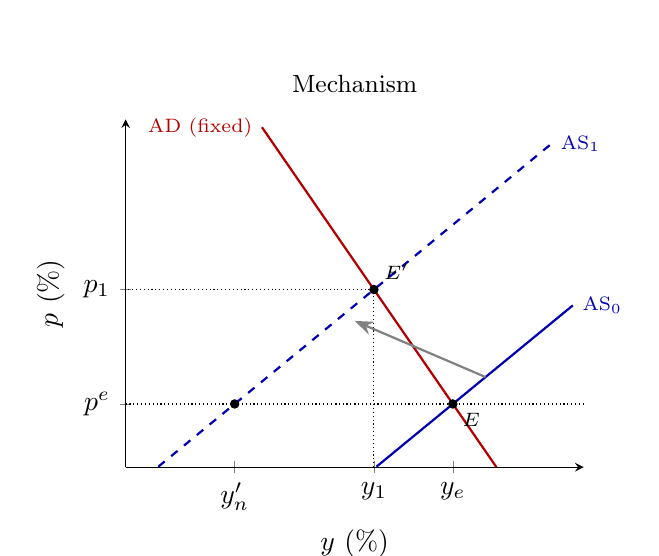
\begin{tikzpicture}
\begin{axis}[width=7.4cm,height=6cm,axis lines=left,xmin=-3,xmax=1.2,ymin=-0.8,ymax=3.6,clip=false,
  xlabel={$y$ (\%)},ylabel={$p$ (\%)},xtick={-2,-0.7234,0},xticklabels={$y_n'$,$y_1$,$y_e$},
  ytick={0,1.4468},yticklabels={$p^e$,$p_1$},title={\small Mechanism}]
\addplot[densely dotted,domain=-3:1.2]{0};
\addplot[thick,blue!70!black,domain=-0.7:1.1]{1.1333*x};
\addplot[thick,blue!70!black,dashed,domain=-2.7:0.9]{1.1333*(x+2)};
\addplot[thick,red!70!black,domain=-1.75:0.4]{-2*x};
\node[font=\scriptsize,blue!70!black,anchor=west] at (axis cs:1.1,1.25) {AS$_0$};
\node[font=\scriptsize,blue!70!black,anchor=west] at (axis cs:0.9,3.29) {AS$_1$};
\node[font=\scriptsize,red!70!black,anchor=east] at (axis cs:-1.75,3.5) {AD (fixed)};
\addplot[only marks,mark=*,mark size=1.5pt] coordinates {(0,0) (-0.7234,1.4468) (-2,0)};
\node[font=\scriptsize,anchor=north west] at (axis cs:0,0) {$E$};
\node[font=\scriptsize,anchor=south west] at (axis cs:-0.72,1.45) {$E'$};
\draw[densely dotted] (axis cs:-0.7234,-0.8)--(axis cs:-0.7234,1.4468)--(axis cs:-3,1.4468);
\draw[-{Stealth},thick,gray] (axis cs:0.3,0.34)--(axis cs:-0.9,1.05);
\end{axis}
\end{tikzpicture}\quad
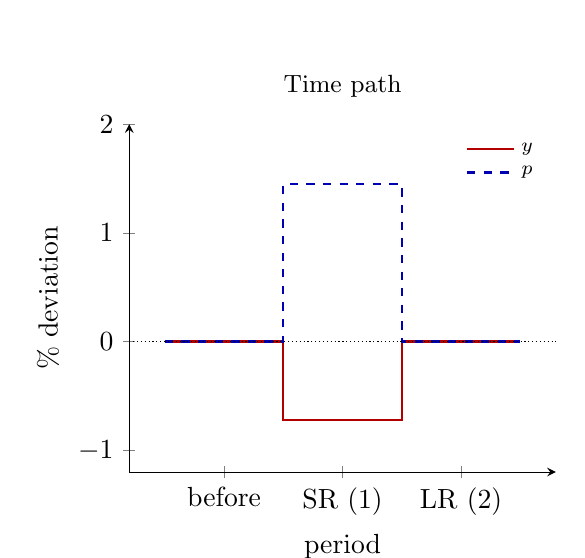
\begin{tikzpicture}
\begin{axis}[width=7cm,height=6cm,axis lines=left,xmin=-0.3,xmax=3.3,ymin=-1.2,ymax=2,
  xlabel={period},xtick={0.5,1.5,2.5},xticklabels={before,SR (1),LR (2)},ylabel={\% deviation},
  title={\small Time path},legend style={font=\scriptsize,draw=none,at={(0.98,0.98)},anchor=north east}]
\addplot[thick,red!70!black,const plot] coordinates {(0,0) (1,-0.7234) (2,0) (3,0)};
\addplot[thick,blue!70!black,dashed,const plot] coordinates {(0,0) (1,1.4468) (2,0) (3,0)};
\addplot[densely dotted,domain=-0.3:3.3]{0};
\legend{$y$,$p$}
\end{axis}
\end{tikzpicture}
\end{center}
\intuicao{The mark-up raises prices at any output; with $\bar p$ anchored, a higher $p$ is a higher real
rate, so demand falls along AD. Output does not fall all the way to $y_n'$ because the sticky firms keep
selling at $p^e$.}
\refbib{Benigno (2015), \S7, Fig.~9, pp.~513--514; \S5, eqs.~(20)--(21).}
\rubrica{
\item AS shifts up/left and AD explicitly does \emph{not} move, with reasons: 1.5 pts.
\item $y=-0.72$, $p=+1.45$: 1 pt (slip: $-1$ pt).
\item Both gaps with opposite signs: 1 pt.
\item Diagram: axes, AS$_0$, AS$_1$ and the unmoved AD labelled, direction of shift: 1 pt; time path SR/LR: 0.5 pt.
\item Shifting AD: max.\ 2 pts on the item. Reporting a single ``output gap'': max.\ 3.5 pts.
}
\end{sol}

\textbf{b)} (5 points) With $u(C)=\dfrac{C^{1-1/\sigma}}{1-1/\sigma}$, $v(L)=\dfrac{L^{1+\eta}}{1+\eta}$,
$Y=AL$ and $C=Y$, the market's labour-supply condition is $\text{MRS}=A/(1+\mu)$ and the planner's is
$\text{MRS}=A$. Derive both, log-linearise, and show $y_n-y_e=-\mu/(\sigma^{-1}+\eta)$. Explain why sticky
prices play no role, and evaluate the gap for this shock.
\resolespaco
\begin{sol}
\passo{1 --- planner}{$\max_Y u(Y)-v(Y/A)$: $u'(Y)=v'(L)/A\Rightarrow\boxed{\dfrac{v'(L)}{u'(C)}=A}$
(MRS $=$ MRT).}
\passo{2 --- market}{Flexible-price firms set $P=(1+\mu)W/A\Rightarrow W/P=A/(1+\mu)$; the household sets
MRS $=W/P$: $\boxed{\dfrac{v'(L)}{u'(C)}=\dfrac{A}{1+\mu}}$. Same condition up to the wedge $1+\mu$.}
\passo{3 --- logs}{$\ln v'=\eta l=\eta(y-a)$; $\ln u'=-\sigma^{-1}c=-\sigma^{-1}y$. So
$\ln\text{MRS}=\eta(y-a)+\sigma^{-1}y$. Planner: $=a\Rightarrow y_e=\dfrac{(1+\eta)a}{\sigma^{-1}+\eta}$.
Market: $=a-\mu\Rightarrow y_n=\dfrac{(1+\eta)a-\mu}{\sigma^{-1}+\eta}$.}
\passo{4 --- subtract}{$\boxed{y_n-y_e=-\dfrac{\mu}{\sigma^{-1}+\eta}}=-\dfrac{4.4}{2.2}=\boxed{-2\%}$.}
\passo{5 --- no stickiness}{$\alpha$ appears in neither condition: $y_n$ is the equilibrium when
\emph{all} prices are flexible; $y_e$ is the planner's, with no prices at all. \#~Stickiness explains
$y\neq y_n$ (it sits in $\kappa$); market power and taxes explain $y_n\neq y_e$. A productivity shock
moves both by $(1+\eta)/(\sigma^{-1}+\eta)$: efficient, no gap.}
\intuicao{A firm with market power pays labour $A/(1+\mu)$ of what it produces; households work until
their MRS equals what they are paid, not what they produce, so the market works and produces too little.}
\refbib{Benigno (2015), \S4.1--\S4.4, eqs.~(14), (15), (19), pp.~507--509.}
\rubrica{
\item Planner MRS $=A$ and market MRS $=A/(1+\mu)$ derived: 2 pts.
\item Log-linearisation and the boxed gap: 1.5 pts; $-2\%$: 0.5 pt.
\item Why stickiness plays no role: 1 pt.
\item Attributing $y_n\neq y_e$ to sticky prices: max.\ 2 pts on the item.
}
\end{sol}

\textbf{c)} (5 points) The Copom minimises $\mathcal L=\phi_y(y-y_e)^2+\phi_p(p-p^e)^2$ with Benigno's
welfare weights $\phi_y=\tfrac12$, $\phi_p=\theta/(2\kappa)$, subject to AS. Derive the targeting rule by
substitution, the optimal $y$ and $p$ and the split of the shock, and the Selic that implements it.
Explain why AS and not AD is the constraint, and what the money market does. Is the optimal response a
rise or a cut relative to doing nothing, and on what does that sign depend?
\resolespaco
\begin{sol}
\passo{1 --- substitute AS}{$\mathcal L(y)=\phi_y y^2+\phi_p\kappa^2(y-y_n)^2$ (with $y_e=0$).
FOC: $\phi_y y+\phi_p\kappa^2(y-y_n)=0$; using $\kappa(y-y_n)=p-p^e$:
$\boxed{\phi_y(y-y_e)+\kappa\phi_p(p-p^e)=0}$; with the welfare weights, $(y-y_e)+\theta(p-p^e)=0$.}
\passo{2 --- optimum}{$\phi_p\kappa^2/\phi_y=\theta\kappa=8\cdot1.133=9.067$.
$y^o=\dfrac{\theta\kappa}{1+\theta\kappa}y_n=0.901\cdot(-2)=\boxed{-1.80\%}$;
$y^o-y_n=\dfrac{2}{1+\theta\kappa}=0.199$; $p^o-p^e=\kappa\cdot0.199=\boxed{+0.23\%}$.
Split: $1/(1+\theta\kappa)=9.9\%$ of the distance $y_e-y_n$ is accepted as output above $y_n$ (hence
prices); $90.1\%$ is absorbed as an output loss. Check: $-1.80+8(0.225)=0$ \checkmark.}
\passo{3 --- the Selic}{Combining AS and AD: $y-y_n=\dfrac{\sigma}{1+\sigma\kappa}(r_n-i)$, with
$r_n=\rho+\sigma^{-1}(\bar y_n-y_n)=5+2\cdot2=9\%$. So
$i^o=9-\dfrac{1.567}{0.5}(0.199)=9-0.623=\boxed{8.38\%}$. Check on AD: $p=5-8.38+2(1.80)=0.23$ \checkmark.
Strict price stability needs $i=r_n=9\%$; strict output stabilisation $i=9-3.133\cdot2=2.73\%$.
Loss: 1.80 at the optimum vs 7.65 with $i=5\%$.}
\passo{4 --- why AS}{One instrument, $i$, which appears only in AD. For any point on AS there is an $i$
that puts AD through it, so AD restricts nothing: it is how the choice is \emph{implemented}. AS is
private pricing behaviour with $p^e$ predetermined, which policy cannot move within the period: it is
the feasible set, like a budget line. The money market has no role in the choice: with $i$ fixed, the
central bank supplies whatever $M=P\,\ell(Y,i)$ is demanded, so it only determines $M$ --- which is why
the model has no LM curve.}
\passo{5 --- sign}{With $i=5\%$, $y-y_n=\dfrac{y_e-y_n}{1+\sigma\kappa}=1.28$; optimum
$\dfrac{y_e-y_n}{1+\theta\kappa}=0.20$. Lower $y-y_n$ needs a higher rate:
\boxed{\text{a rise of }3.38\text{ pp}}. It is a rise iff $\theta\kappa>\sigma\kappa\iff\theta>\sigma$
(general weights: $(\phi_p/\phi_y)\kappa>\sigma$), i.e.\ iff the IT line (slope $-1/\theta$) is flatter
than AD (slope $-1/\sigma$). A dovish bank with $(\phi_p/\phi_y)\kappa<\sigma$ would \emph{cut}.}
\begin{center}
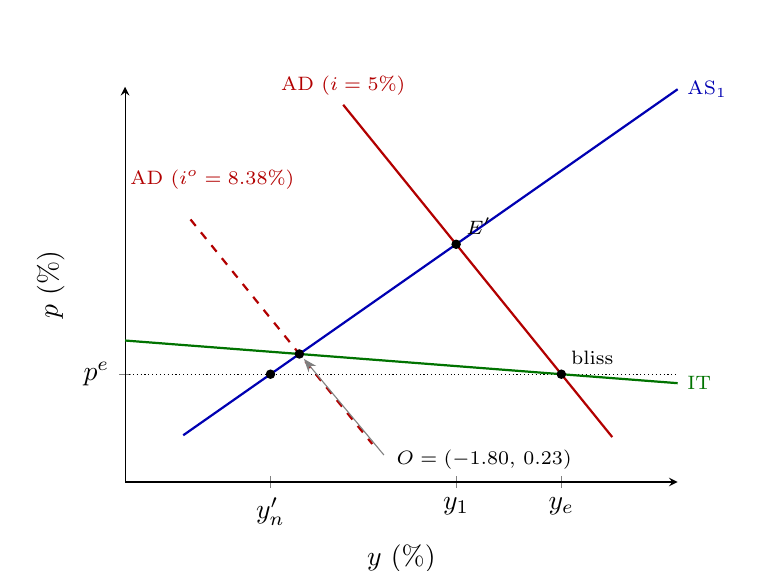
\begin{tikzpicture}
\begin{axis}[width=8.6cm,height=6.6cm,axis lines=left,xmin=-3,xmax=0.8,ymin=-1.2,ymax=3.2,clip=false,
  xlabel={$y$ (\%)},ylabel={$p$ (\%)},xtick={-2,-0.7234,0},xticklabels={$y_n'$,$y_1$,$y_e$},
  ytick={0},yticklabels={$p^e$}]
\addplot[densely dotted,domain=-3:0.8]{0};
\addplot[thick,blue!70!black,domain=-2.6:0.8]{1.1333*(x+2)};
\addplot[thick,green!45!black,domain=-3:0.8]{-x/8};
\addplot[thick,red!70!black,domain=-1.5:0.35]{-2*x};
\addplot[thick,red!70!black,dashed,domain=-2.55:-1.3]{-3.377-2*x};
\node[font=\scriptsize,blue!70!black,anchor=west] at (axis cs:0.8,3.17) {AS$_1$};
\node[font=\scriptsize,green!45!black,anchor=west] at (axis cs:0.8,-0.1) {IT};
\node[font=\scriptsize,red!70!black,anchor=south] at (axis cs:-1.5,3.0) {AD ($i=5\%$)};
\node[font=\scriptsize,red!70!black,anchor=south] at (axis cs:-2.4,1.95) {AD ($i^o=8.38\%$)};
\addplot[only marks,mark=*,mark size=1.5pt] coordinates {(-0.7234,1.4468) (-1.8013,0.2252) (0,0) (-2,0)};
\node[font=\scriptsize,anchor=south west] at (axis cs:-0.72,1.45) {$E'$};
\node[font=\scriptsize,anchor=west] at (axis cs:-1.2,-0.95) {$O=(-1.80,\,0.23)$};
\draw[-{Stealth},gray] (axis cs:-1.22,-0.9)--(axis cs:-1.77,0.17);
\node[font=\scriptsize,anchor=south west] at (axis cs:0,0) {bliss};
\end{axis}
\end{tikzpicture}\\
{\footnotesize The optimum $O$ is where AS$_1$ meets the IT line $(y-y_e)+\theta(p-p^e)=0$; the Copom raises $i$ so that AD shifts
down/left from $E'$ to $O$. AS does not move with policy.}
\end{center}
\intuicao{A mark-up shock moves $y_n$ but not $y_e$, so no rate delivers both targets. Convex losses
make the bank spread the miss; with welfare weights, relative-price dispersion is so costly
($\theta=8$) that it lets only a tenth of the shock into prices.}
\refbib{Benigno (2015), \S11, eqs.~(33)--(35), Fig.~14, pp.~521--523; \S3 on the interest-rate instrument.}
\rubrica{
\item Targeting rule by substitution: 1.5 pts.
\item $y^o=-1.80$, $p^o=+0.23$, split $1/(1+\theta\kappa)$: 1 pt (slip: $-1$ pt).
\item $i^o=8.38\%$ via $r_n=9\%$: 0.5 pt.
\item Why AS is the constraint and the money market determines $M$: 1 pt.
\item Sign relative to no policy with the condition $\theta>\sigma$: 1 pt.
\item Using AD as the constraint: max.\ 2 pts on the item. Targeting $y_n$ instead of $y_e$: max.\ 2.5 pts.
}
\gap{Lista 7 (latest content): a temporary mark-up shock moves only AS; $y-y_n$ vs $y-y_e$; why
$y_n\neq y_e$ (wedge, not stickiness); optimal policy subject to AS and why AD is not a constraint.
Lista 6, 1(d): under a rate instrument the money market determines $M$.}
\end{sol}

\ifsolucoes\else
\vfill
\begin{center}\footnotesize\textit{End of exam.}\end{center}
\fi

\end{document}
"   (run twice)
% Check fonts: pdffonts <file>.pdf  (all Type 1).
% Every number in the key: python simulado_codigo/check_simulado_02.py
% =============================================================================
\documentclass[11pt,a4paper]{article}
\usepackage[utf8]{inputenc}
\usepackage[T1]{fontenc}
\usepackage{lmodern}   % Type 1 vector fonts (replaces PK bitmaps)
\usepackage{cmap}      % ToUnicode CMap -> copyable text and accents
\usepackage[english]{babel}
\usepackage{amsmath,amssymb,amsfonts}
\usepackage[a4paper,margin=2.2cm]{geometry}
\usepackage{enumitem}
\usepackage{fancyhdr}
\usepackage{comment}
\usepackage{xcolor}
\usepackage{microtype}
\usepackage{booktabs}
\usepackage{needspace}
\usepackage{pgfplots}
\pgfplotsset{compat=1.18}
\usetikzlibrary{arrows.meta}

% ====================== CONFIGURATION ======================
\newif\ifsolucoes
\ifdefined\withsolutions\solucoestrue\else\solucoesfalse\fi

\newcommand{\disciplina}{Macroeconomics I --- MPE Insper}
\newcommand{\listatema}{Mock Final Exam 2}
\newcommand{\espacoresol}{6.5cm}

% ====================== MACHINERY ======================
\ifsolucoes\includecomment{sol}\else\excludecomment{sol}\fi

\pagestyle{fancy}\fancyhf{}
\lhead{\footnotesize\disciplina}
\rhead{\footnotesize \listatema\ifsolucoes{} --- Solutions and Rubric\fi}
\cfoot{\footnotesize\thepage}
\renewcommand{\headrulewidth}{0.3pt}
\setlength{\headheight}{14pt}

\setlist{topsep=2pt,itemsep=2pt}
\newcounter{questao}

\newcommand{\bloco}[3]{\Needspace{10\baselineskip}\bigskip\noindent
  {\large\bfseries\color{blue!55!black}Block #1 --- #2}\hfill\textit{(#3)}\par
  \noindent\rule{\linewidth}{0.3pt}\smallskip}
\newcommand{\questao}[1]{\refstepcounter{questao}\medskip\noindent
  \textbf{Question \thequestao.}~#1\par}
\newenvironment{alternativas}{\begin{enumerate}[label=\Alph*.,leftmargin=2.2em,topsep=1pt]}{\end{enumerate}}
\newcommand{\gabarito}[1]{\ifsolucoes\par\noindent\textbf{Answer:}~#1\fi}
\newcommand{\resolespaco}{\ifsolucoes\else\par\textit{Solution:}\vspace{\espacoresol}\par\fi}
\newcommand{\passo}[2]{\par\smallskip\noindent\textbf{Step #1.}~#2}
\newcommand{\intuicao}[1]{\par\smallskip\noindent\textit{Intuition.}~#1}
\newcommand{\refbib}[1]{\par\smallskip\noindent{\footnotesize\color{black!60}\textbf{Ref:} #1}}
\newcommand{\gap}[1]{\par\smallskip\noindent{\footnotesize\color{red!55!black}\textbf{Gap targeted:} #1}}
\newcommand{\trap}[1]{\par\smallskip\noindent{\small\color{red!55!black}\#~#1}}
\newcommand{\rubrica}[1]{\par\smallskip\noindent\textbf{Grading rubric.}\begin{itemize}[leftmargin=1.4em,topsep=1pt]#1\end{itemize}}

% =============================================================================
\begin{document}
\begin{center}
  {\Large\bfseries \disciplina}\\[2pt]
  {\large \listatema\ (Simulado 2) --- 2026, 3rd term}\ifsolucoes\\[2pt]\textit{Solutions and Grading Rubric}\fi
\end{center}
\vspace{2pt}

{\footnotesize\noindent\textbf{Instructions.} Four blocks of 25 points (100 in total). Duration: 3 hours,
closed book, non-programmable calculator allowed. Each block has one objective question (10 points)
and one discursive question (15 points).
\emph{Multiple choice} (items a, b): mark the single correct option; no penalty for a wrong answer.
\emph{True/False} (items c, d): the score of the T/F items is
$\max\{0,\ \text{correct}-\text{wrong}/2\}\times$ item value, i.e.\ every two wrong items cancel one
correct item; blank items do not count as wrong.
\emph{Discursive questions}: show every step; box final answers; sign every derivative before
interpreting it; label axes and curves in diagrams. Notation: Kurlat (2020) in Blocks I--III, Benigno
(2015) in Block IV. All numbers are illustrative.\par}

\ifsolucoes
\medskip
{\footnotesize\noindent\textbf{How the rubric works.} Conceptual caps (``max.\ $x$ pts'') bound an
item whatever else is right. Light penalties ($-1$ pt) apply to arithmetic slips with a correct method.
Caps and penalties are \emph{not cumulative}: when a cap applies, the penalties inside it are ignored.
Each question ends with the graded mistake it retests (``Gap targeted''). Every number below is
recomputed by \texttt{simulado\_codigo/check\_simulado\_02.py}.\par}
\fi

% =============================================================================
\bloco{I}{Measurement and national accounts}{Lecture 1 \,\textbullet\, 25 points}

\questao{(10 points) Objective items.}

\textbf{a)} (3 points) A soy chain in Mato Grosso, one year, values in R\$ million. A fertiliser
producer, which uses no intermediate inputs, sells its whole output, 30, to a soy farm. The farm
harvests soy worth 100: it sells 70 to a crushing plant and exports 30 to China. The crusher sells
soybean oil worth 150 to Brazilian households. By the production (value-added) approach, the chain's
contribution to Brazil's GDP is:
\begin{alternativas}
\item 150
\item 280
\item 180
\item 210
\item 250
\end{alternativas}
\gabarito{C.}
\begin{sol}
Value added $=(30-0)+(100-30)+(150-70)=30+70+80=\boxed{180}$. Check by expenditure:
$C+X=150+30=180$. B (280) is gross production, which counts the intermediate inputs 30 and 70 twice;
A (150) forgets the exports; D (210) subtracts only the soy input; E (250) adds the last two sales.
\refbib{Kurlat ch.~1, \S1.1 (the three approaches), pp.~15--21.}
\end{sol}

\medskip
\textbf{b)} (3 points) IBGE data for a year, in R\$ billion: GDP is 10{,}000; wages earned by
Brazilian residents on short assignments abroad, 50; profits of foreign-owned plants in Brazil sent to
their parent companies, 300; interest on Brazilian bonds held by non-residents, 150; personal transfers
sent home by Brazilians who live permanently abroad, 40. Using Kurlat's definition,
$\text{GNI}=\text{GDP}+F^{\text{out}}-F^{\text{in}}$, where $F^{\text{out}}$ is factor income earned
abroad by residents and $F^{\text{in}}$ factor income earned at home by non-residents, Brazil's GNI is:
\begin{alternativas}
\item 9{,}640
\item 10{,}400
\item 9{,}750
\item 9{,}600
\item 10{,}000
\end{alternativas}
\gabarito{D.}
\begin{sol}
$\text{GNI}=10{,}000+50-300-150=\boxed{9{,}600}$. Profits and interest are \emph{factor} income of
non-residents; the 40 are transfers, not payments to a factor of production, so they are not in GNI
(A adds them). B flips the signs; C leaves the interest out; E confuses territory (GDP) with
ownership (GNI).
\refbib{Kurlat ch.~1, \S1.1, GDP vs GNP.}
\end{sol}

\medskip
\textbf{c)} (2 points, T or F) In a year in which Brazil's gross fixed capital formation equals
17\% of GDP, Brazil's stock of fixed capital rises by 17\% of GDP.
\gabarito{F.}
\begin{sol}
Investment is a gross \emph{flow}; the stock changes by the net flow, $K_{t+1}-K_t=I_t-\delta K_t$.
With, say, $K/Y=3$ and $\delta=4\%$, $\delta K=12\%$ of GDP is replacement, and the stock rises by
only $17-12=5\%$ of GDP.
\refbib{Kurlat ch.~1, eq.~(1.2) and the depreciation discussion, p.~21.}
\end{sol}

\medskip
\textbf{d)} (2 points, T or F) In 2015 Brazil's nominal GDP grew by about 3.8\% while real GDP fell by
about 3.5\%. Hence the GDP deflator rose by less than 3.8\% that year.
\gabarito{F.}
\begin{sol}
$1+\pi_{\text{defl}}=\dfrac{1+g_{\text{nominal}}}{1+g_{\text{real}}}=\dfrac{1.038}{0.965}=1.0756$, so
$\boxed{\pi_{\text{defl}}\approx7.6\%>3.8\%}$. When real output falls, the deflator must grow
\emph{faster} than nominal GDP, not slower.
\refbib{Kurlat ch.~1, \S1.2 (real vs nominal), pp.~22--25.}
\end{sol}
\begin{sol}
\gap{Lista 1, 1(b)--(c): both lost marks were numbers that changed between the line computing them
and the line using them. Items (a) and (d) reward copying each intermediate result exactly.}
\end{sol}

% -----------------------------------------------------------------------------
\questao{(15 points) Brazil and Portugal: exchange rates, prices and welfare.
A think tank compares living standards in Brazil and Portugal with a two-good economy. Per-capita
annual quantities and local prices are:}

\begin{center}\small
\begin{tabular}{@{}lcccc@{}}
\toprule
& \multicolumn{2}{c}{Traded good $T$ (grains, manufactures)} & \multicolumn{2}{c}{Non-traded good $N$ (housing, haircuts, services)}\\
& quantity & price & quantity & price \\
\midrule
Brazil & 5 & 10 reais & 10 & 4 reais \\
Portugal & 10 & 2 euros & 15 & 2 euros \\
\bottomrule
\end{tabular}
\end{center}
\noindent The traded good obeys the law of one price at the market exchange rate. Output per worker is
$A_T=2$, $A_N=5$ in Brazil and $A_T=A_N=5$ in Portugal; within each country labour moves freely between
sectors and firms are competitive.

\textbf{a)} (5 points) Find the market exchange rate (reais per euro), Brazil's GDP per capita in
euros at the market rate and at PPP (Brazil's quantities valued at Portuguese prices), the
Brazil/Portugal ratio under each conversion, the PPP exchange rate and Brazil's price level relative
to Portugal's.
\resolespaco
\begin{sol}
\passo{1 --- market rate}{Law of one price in $T$: 10 reais $=$ 2 euros, so
$\boxed{e=5\text{ reais per euro}}$.}
\passo{2 --- nominal GDP per capita}{Brazil: $5\cdot10+10\cdot4=50+40=90$ reais. Portugal:
$10\cdot2+15\cdot2=20+30=50$ euros.}
\passo{3 --- market-rate conversion}{Brazil $=90/5=18$ euros; ratio $18/50=\boxed{0.36}$.}
\passo{4 --- PPP conversion}{Brazil at Portuguese prices: $5\cdot2+10\cdot2=10+20=30$ euros; ratio
$30/50=\boxed{0.60}$.}
\passo{5 --- PPP rate and price level}{$e^{\text{PPP}}=90/30=\boxed{3\text{ reais per euro}}$.
Relative price level $=e^{\text{PPP}}/e=3/5=\boxed{0.6}$: Brazil's basket costs 60\% of what it costs in
Portugal.}
\passo{6 --- check}{$0.60/0.36=1.667=1/0.6$: the two ratios differ exactly by the price level.}
\refbib{Kurlat ch.~1, \S1.2, international comparisons and PPP, pp.~25--27.}
\rubrica{
\item $e=5$: 1 pt. Market-rate ratio 0.36: 1 pt. PPP ratio 0.60: 1.5 pts. $e^{\text{PPP}}=3$ and price level 0.6: 1.5 pts.
\item Valuing Portugal at Brazilian prices instead is a legitimate PPP (ratio $90/(10\cdot10+15\cdot4)=0.5625$) if stated: full marks for that part; unstated mix of bases: max.\ 3 pts.
\item Arithmetic slip with correct method: $-1$ pt.
}
\end{sol}

\textbf{b)} (5 points) Which good drives the gap between the two ratios? Derive the relative price of
the non-traded good in each country from the firms' and workers' conditions, explain the direction of
the bias of the market-rate comparison (Balassa--Samuelson), and explain why ``transport and trade
costs'' is \emph{not} the explanation here.
\resolespaco
\begin{sol}
\passo{1 --- split Brazil's output by good}{Traded: $50/5=10$ euros at the market rate and
$5\cdot2=10$ euros at PPP --- identical. Non-traded: $40/5=8$ euros at the market rate and
$10\cdot2=20$ euros at PPP. \boxed{\text{The whole 12-euro gap comes from the non-traded good.}}}
\passo{2 --- wage equalisation}{Competitive firms pay the value of the marginal product and workers
move until wages are equal: $W=p_TA_T=p_NA_N\;\Rightarrow\;\boxed{p_N/p_T=A_T/A_N}$.
Brazil: $2/5=0.4=4/10$ \checkmark. Portugal: $5/5=1=2/2$ \checkmark.}
\passo{3 --- mechanism}{$A_T^{BR}/A_T^{PT}=0.4$ while $A_N^{BR}/A_N^{PT}=1$: Brazil's productivity gap
is in traded goods.
$A_T\downarrow\;\rightarrow\;W=p_TA_T\downarrow$ (with $p_T$ tied to the world price)
$\rightarrow\;p_N=W/A_N\downarrow\;\rightarrow$ non-traded goods are cheap in Brazil
$\rightarrow$ the market rate values Brazil's non-traded output at a price nobody pays in Portugal.}
\passo{4 --- direction}{\boxed{\text{The market rate understates Brazil's real output}} (0.36 vs 0.60),
and more so the larger the productivity gap in $T$ relative to $N$. A uniform gap in both sectors
would leave $A_T/A_N$ and hence the price level unchanged.}
\passo{5 --- why not trade costs}{Trade costs are frictions on \emph{traded} goods, and in this
economy the law of one price holds exactly for $T$ --- where the market rate works perfectly (Step 1).
The bias sits in the good that is never traded, for which there is no arbitrage at \emph{any} trade
cost. Trade costs would also push the importer's price up, not produce a systematic ``poorer is
cheaper'' pattern.}
\intuicao{Wages are set by productivity in the sector that faces world prices, and the same wage is
paid to haircutters whose productivity is the same everywhere. Cheap services in poor countries are a
wage fact, not a transport fact.}
\refbib{Kurlat ch.~1, \S1.2, pp.~25--27; Balassa--Samuelson as derived in the course notes
(\texttt{Map/aula-01-mensuracao/04}).}
\rubrica{
\item Decomposition showing the gap is entirely in $N$: 1.5 pts.
\item $p_N/p_T=A_T/A_N$ from wage equalisation, both countries checked: 1.5 pts.
\item Direction (understates) with the mechanism in words: 1 pt.
\item Why trade costs fail: 1 pt.
\item Explaining the gap by trade/import costs: max.\ 2 pts on the item (conceptual cap).
}
\end{sol}

\textbf{c)} (5 points) Welfare beyond GDP. Use Kurlat's consumption-equivalent (Jones--Klenow)
measure with log utility ($\sigma=1$), lognormal consumption within each country and equal leisure
(set the leisure term to zero). A person lives in a country with probability $e=\text{LE}/100$ and then
enjoys $\bar u+\mathbb E[\ln c]$. Data: Brazil's mean consumption per capita is 60\% of Portugal's
(normalise Portugal's to 1); the standard deviation of log consumption is $s_{BR}=0.9$ and
$s_{PT}=0.5$; life expectancy is 76 and 81 years; $\bar u=5$. Find $\lambda$, the factor applied to
Portuguese consumption that makes a person behind the veil indifferent between the two countries,
decompose $\ln\lambda$ into consumption, inequality and life-expectancy terms, and compare with (a).
\resolespaco
\begin{sol}
\passo{1 --- set-up}{Indifference:
$e_{PT}\left[\bar u+\ln\lambda+\mathbb E\ln c_{PT}\right]=e_{BR}\left[\bar u+\mathbb E\ln c_{BR}\right]$.
Lognormal: $\mathbb E\ln c=\ln\bar c-\tfrac12s^2$.}
\passo{2 --- ingredients}{$\mathbb E\ln c_{PT}=0-\tfrac12(0.25)=-0.125$;
$\mathbb E\ln c_{BR}=\ln0.6-\tfrac12(0.81)=-0.5108-0.405=-0.9158$.
Flow values: $v_{PT}=5-0.125=4.875$, $v_{BR}=5-0.9158=4.0842$.}
\passo{3 --- solve}{$\ln\lambda=\dfrac{e_{BR}}{e_{PT}}v_{BR}-v_{PT}=\dfrac{76}{81}(4.0842)-4.875
=0.93827\cdot4.0842-4.875=3.8321-4.875=\boxed{-1.043}$, so $\boxed{\lambda=e^{-1.043}\approx0.35}$.}
\passo{4 --- decomposition}{$\ln\lambda=\underbrace{\ln0.6}_{\text{consumption}}
\underbrace{-\tfrac12(0.81-0.25)}_{\text{inequality}}
+\underbrace{\left(\tfrac{76}{81}-1\right)4.0842}_{\text{life expectancy}}
=-0.511-0.280-0.252=-1.043$ \checkmark\ (exact, not an approximation).}
\passo{5 --- comparison}{The PPP ratio 0.60 is the right GDP benchmark; welfare is lower, 0.35,
because inequality and shorter lives add $0.53$ log points to the gap. That 0.35 is close to the
market-rate ratio 0.36 is a coincidence: the market rate is wrong for a price reason (b); $\lambda$ is
low for inequality and mortality reasons.}
\intuicao{Behind the veil, inequality is risk, and log utility prices it at half the log variance;
a shorter life scales down every year's utility, weighted by the value of being alive, $\bar u$.}
\refbib{Kurlat ch.~2, \S2.2 (Jones--Klenow), eqs.~(2.2.1)--(2.2.3), pp.~33--41.}
\rubrica{
\item Indifference condition written with $e$ multiplying the whole bracket: 1.5 pts.
\item $\mathbb E\ln c=\ln\bar c-s^2/2$ used for both countries: 1 pt.
\item $\ln\lambda=-1.043$, $\lambda\approx0.35$: 1 pt; three terms: 1 pt.
\item Comparison with 0.60 (not 0.36) as the benchmark: 0.5 pt.
\item Treating life expectancy additively (not as a probability weight): max.\ 2.5 pts.
\item Reading $\lambda\approx0.36$ as vindicating the market rate: $-1$ pt.
}
\gap{Lista 1, 1(e): the PPP gap was explained with import/export costs; the mark is for
non-tradables and Balassa--Samuelson. Also Lista 1's rule ``answer every object'': (a) asks for five
numbers.}
\end{sol}

% =============================================================================
\bloco{II}{Long-run growth and the Solow model}{Lectures 2--3 \,\textbullet\, 25 points}

\questao{(10 points) Objective items.}

\textbf{a)} (3 points) Solow model in \emph{per-worker} terms, no technological progress,
$Y=K^{1/3}L^{2/3}$, $s=0.20$, $\delta=0.05$. Starting from its steady state, Brazil's population growth
falls permanently from 2\% to 1\% a year (the demographic transition). Which statement about
steady-state output per worker $y^\ast$, the growth of $y$ during the transition and the growth of
aggregate $Y$ in the new steady state is correct?
\begin{alternativas}
\item $y^\ast$ rises by about 26.0\%; $g_y>0$ only during the transition; $g_Y$ falls from 2\% to 1\%.
\item $y^\ast$ rises by about 8.0\%; $g_y>0$ only during the transition; $g_Y$ stays at 2\%.
\item $y^\ast$ rises by about 8.0\%; $g_y$ is permanently higher than before; $g_Y$ stays at 2\%.
\item $y^\ast$ rises by about 16.7\%; $g_y>0$ only during the transition; $g_Y$ falls from 2\% to 1\%.
\item $y^\ast$ rises by about 8.0\%; $g_y>0$ only during the transition; $g_Y$ falls from 2\% to 1\%.
\end{alternativas}
\gabarito{E.}
\begin{sol}
$k^\ast=\left(\dfrac{s}{n+\delta}\right)^{\frac{1}{1-\alpha}}$, $y^\ast=\left(\dfrac{s}{n+\delta}\right)^{\frac{\alpha}{1-\alpha}}
=\left(\dfrac{s}{n+\delta}\right)^{1/2}$, so
$\dfrac{y^\ast_{new}}{y^\ast_{old}}=\left(\dfrac{0.07}{0.06}\right)^{1/2}=1.080$: $\boxed{+8.0\%}$.
The flatter break-even line $(n'+\delta)k$ leaves $sf(k)>(n'+\delta)k$ at the old $k^\ast$, so $k$ and
$y$ grow until the new steady state and then $g_y=0$ again. Aggregate $Y=yL$ grows at $g_y+n$: $n$
before, $n'$ after. \#~Higher level, same (zero) steady-state per-worker growth, higher growth during
convergence, \emph{lower} aggregate growth. A uses $k^\ast$ ($+26.0\%$); D uses the ratio of
break-even slopes ($+16.7\%$); B and C forget aggregate vs per worker.
\end{sol}
\begin{sol}
\begin{center}
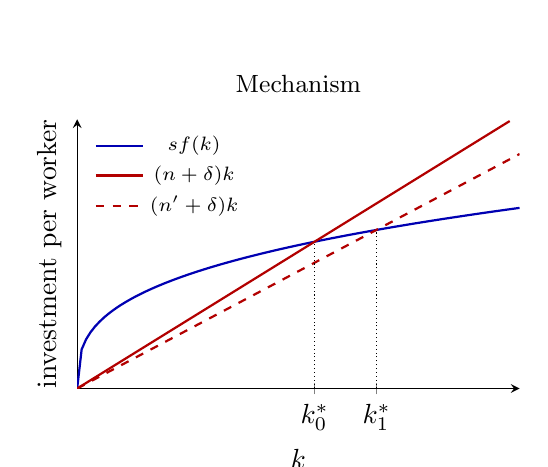
\begin{tikzpicture}
\begin{axis}[width=7.2cm,height=5cm,axis lines=left,xmin=0,xmax=9,ymin=0,ymax=0.62,
  xlabel={$k$},ylabel={investment per worker},xtick={4.83,6.09},xticklabels={$k^\ast_0$,$k^\ast_1$},
  ytick=\empty,title={\small Mechanism},legend style={font=\scriptsize,at={(0.02,0.98)},anchor=north west,draw=none}]
\addplot[thick,blue!70!black,domain=0:9,samples=100]{0.2*x^(1/3)};
\addplot[thick,red!70!black,domain=0:8.8]{0.07*x};
\addplot[thick,red!70!black,dashed,domain=0:9]{0.06*x};
\legend{$sf(k)$,$(n+\delta)k$,$(n'+\delta)k$}
\draw[densely dotted] (axis cs:4.83,0)--(axis cs:4.83,0.338);
\draw[densely dotted] (axis cs:6.09,0)--(axis cs:6.09,0.365);
\end{axis}
\end{tikzpicture}\quad
\begin{tikzpicture}
\begin{axis}[width=7.2cm,height=5cm,axis lines=left,xmin=-10,xmax=60,ymin=0.5,ymax=0.63,
  xlabel={time},ylabel={$\ln y$},xtick={0},xticklabels={$t_0$},ytick={0.525,0.602},
  yticklabels={$\ln y^\ast_0$,$\ln y^\ast_1$},title={\small Time path}]
\addplot[thick,blue!70!black,domain=-10:0]{0.5249};
\addplot[thick,blue!70!black,domain=0:60,samples=60]{0.6019-(0.6019-0.5249)*exp(-0.04*x)};
\addplot[densely dotted,domain=-10:60]{0.6019};
\end{axis}
\end{tikzpicture}
\end{center}
{\footnotesize Left: $n$ falls, the break-even ray rotates down, $k^\ast$ rises. Right: $\ln y$ rises
during the transition and flattens; $\ln Y$ (not drawn) has slope $n=2\%$ before and $n'=1\%$ after.}
\refbib{Kurlat ch.~4, \S4.2 (comparative statics), pp.~59--61.}
\end{sol}

\medskip
\textbf{b)} (3 points) Same model with $\alpha=0.35$ and $n+\delta=0.07$; Brazil saves 17\% of GDP.
Which statement is correct about the golden-rule saving rate and the effect on steady-state
consumption per worker of raising $s$ from 0.17 to 0.25?
\begin{alternativas}
\item $s_{GR}=0.65$; raising $s$ from 0.17 to 0.25 lowers steady-state consumption per worker.
\item $s_{GR}=0.35$; raising $s$ from 0.17 to 0.25 raises steady-state consumption per worker.
\item $s_{GR}=0.35$; raising $s$ from 0.17 to 0.25 lowers steady-state consumption per worker.
\item $s_{GR}=1.00$; raising $s$ from 0.17 to 0.25 raises steady-state consumption per worker.
\end{alternativas}
\gabarito{B.}
\begin{sol}
$c^\ast=f(k^\ast)-(n+\delta)k^\ast$ is maximised at $f'(k_{GR})=n+\delta$; with Cobb--Douglas
$\alpha k^{\alpha-1}=n+\delta$ and $s\,k^{\alpha-1}=n+\delta$ give $\boxed{s_{GR}=\alpha=0.35}$.
$c^\ast(s)=(1-s)\left(\frac{s}{0.07}\right)^{0.35/0.65}$: $c^\ast(0.17)=1.338<c^\ast(0.25)=1.488$.
Below the golden rule a higher $s$ raises long-run consumption (after an initial fall). A uses
$1-\alpha$; C reads only the $(1-s)$ factor; D maximises $k^\ast$, not $c^\ast$.
\refbib{Kurlat ch.~4, \S4.3 (golden rule), pp.~61--63.}
\end{sol}

\medskip
\textbf{c)} (2 points, T or F) Of two economies with the same technology, depreciation and population
growth, the one with lower capital per worker necessarily grows faster.
\gabarito{F.}
\begin{sol}
Convergence is \emph{conditional}: $g_k=s\,k^{\alpha-1}-(n+\delta)$ depends on the distance to each
economy's own steady state, which depends on $s$. With $\alpha=1/3$, $n+\delta=0.07$: $X$ with $k=3$,
$s=0.10$ has $g_k=-2.2\%$; $Z$ with $k=5$, $s=0.30$ has $g_k=+3.3\%$.
\refbib{Kurlat ch.~5, \S5.1--\S5.3 (convergence), pp.~75--86.}
\end{sol}

\medskip
\textbf{d)} (2 points, T or F) If a country's national accounts show a capital share of income of one
third, the same as in undistorted economies with $\alpha=1/3$, then its measured TFP reflects only
technology.
\gabarito{F.}
\begin{sol}
Normal factor shares do not rule out distortions. A requirement to hold unproductive capital recorded
as capital leaves $rK/Y=\alpha$ exactly and puts the whole distortion in the residual,
$\hat A=A(1+\theta)^{-\alpha}$ (Question 4).
\refbib{Kurlat ch.~5, \S5.4--\S5.5 (growth and development accounting), pp.~86--95.}
\gap{Lista 1, 4(b): a Solow comparative static in $n$ left blank; Lista 1, 4(a): aggregate vs per
capita (item a). Item (d) previews Lista 2, 2(c).}
\end{sol}

% -----------------------------------------------------------------------------
\questao{(15 points) ``Custo Brasil'' in the growth accounts.
Output is $Y=AK_P^{\alpha}L^{1-\alpha}$ with $\alpha=0.4$, where $K_P$ is productive capital.
Regulation, legal uncertainty and crime force every firm to hold $\theta$ units of \emph{compliance
capital} (duplicate tax-filing systems, armoured vehicles, walls, back-up generators) for each unit of
productive capital. Compliance capital produces nothing, but the national accounts record it as capital
like any other, so measured capital is $K=K_P+\theta K_P$. Capital is rented at $r$ and labour hired
at $w$ in competitive markets. Today $\theta=0.6$.}

\textbf{a)} (5 points) Write aggregate output as a function of $A,K,L,\theta$. What share of measured
capital is unproductive? How much output is lost relative to an economy with $\theta=0$ and the same
$A,K,L$? State the base of your percentage.
\resolespaco
\begin{sol}
\passo{1 --- composition}{$K=(1+\theta)K_P\Rightarrow K_P=K/(1+\theta)$.}
\passo{2 --- output}{$Y=A\left(\dfrac{K}{1+\theta}\right)^{\alpha}L^{1-\alpha}
\;\Rightarrow\;\boxed{Y=\underbrace{A(1+\theta)^{-\alpha}}_{\text{wedge on TFP}}K^{\alpha}L^{1-\alpha}}$.}
\passo{3 --- unproductive share}{$\dfrac{\theta K_P}{(1+\theta)K_P}=\dfrac{0.6}{1.6}=\boxed{37.5\%}$.}
\passo{4 --- output lost}{$\dfrac{Y(\theta)}{Y(0)}=(1.6)^{-0.4}=e^{-0.4\ln1.6}=e^{-0.4\cdot0.4700}=e^{-0.1880}=0.8286$.
\boxed{\text{Output is }17.1\%\text{ below the undistorted level}} (base: $Y(0)$). Equivalently,
removing $\theta$ would raise output by $1/0.8286-1=\boxed{20.7\%}$ (base: $Y(\theta)$).
\#~Careful with the chosen base.}
\intuicao{A third of the capital stock does no work, but output falls by less than a third because
capital has diminishing returns and a share of only 0.4.}
\refbib{Kurlat ch.~5, \S5.4--\S5.5, pp.~86--95.}
\rubrica{
\item $K_P=K/(1+\theta)$ and the boxed $Y$ with the wedge named: 2 pts.
\item Share 37.5\%: 1 pt.
\item Loss 17.1\% (or gain 20.7\%) with the base stated: 2 pts; no base stated: $-1$ pt.
\item Loss computed as $\theta/(1+\theta)=37.5\%$ of output: max.\ 2 pts on the item.
}
\end{sol}

\textbf{b)} (5 points) Write the representative firm's problem and first-order conditions and derive
the measured factor shares $rK/Y$ and $wL/Y$. A development accountant has data on $Y$, $K$, $L$ and
factor payments only. What does she conclude about $\alpha$ and about TFP? Who bears the cost of
$\theta$?
\resolespaco
\begin{sol}
\passo{1 --- problem}{To use $K_P$ productive units the firm must rent $(1+\theta)K_P$:
$\max_{K_P,L}\;AK_P^{\alpha}L^{1-\alpha}-r(1+\theta)K_P-wL$.}
\passo{2 --- FOCs}{$\alpha\dfrac{Y}{K_P}=r(1+\theta)$ and $(1-\alpha)\dfrac{Y}{L}=w$.}
\passo{3 --- shares}{Using $(1+\theta)K_P=K$: $r=\dfrac{\alpha Y}{(1+\theta)K_P}=\alpha\dfrac{Y}{K}$, so
$\boxed{rK/Y=\alpha=0.4}$ and $\boxed{wL/Y=1-\alpha=0.6}$: \emph{undistorted}.}
\passo{4 --- the accountant}{She sets $\hat\alpha=rK/Y=0.4=\alpha$ (correct) and computes
$\hat A=\dfrac{Y}{K^{\hat\alpha}L^{1-\hat\alpha}}=\boxed{A(1+\theta)^{-\alpha}=0.83A}$.
She concludes that Brazil has 17\% lower \emph{technology}. Wrong: technology is $A$; the gap is a
wasted-capital distortion that the data classify as productivity.}
\passo{5 --- incidence}{The rental rate $r=\alpha Y/K$ and the wage
$w=(1-\alpha)\hat A(K/L)^{\alpha}$ are both lower at given $K/L$ by the factor $(1+\theta)^{-\alpha}$.
\#~Workers are also affected: capital and labour are complements.}
\intuicao{Each productive machine drags $\theta$ idle ones with it, so capital looks less productive
by exactly the amount it is paid less: the share is untouched, the level is not.}
\refbib{Kurlat ch.~5, \S5.4 (factor shares and TFP), pp.~86--92.}
\rubrica{
\item Problem with cost $r(1+\theta)K_P$ and both FOCs: 1.5 pts.
\item $rK/Y=\alpha$, $wL/Y=1-\alpha$: 1.5 pts.
\item $\hat\alpha=\alpha$ and $\hat A=A(1+\theta)^{-\alpha}$, read as distortion, not technology: 1.5 pts.
\item Workers also bear the cost: 0.5 pt.
\item Claiming the capital share is distorted ($\hat\alpha\neq\alpha$): max.\ 2 pts on the item.
}
\end{sol}

\textbf{c)} (5 points) A reform (tax simplification, digital filing, lower crime) cuts $\theta$ from
0.6 to 0.28 gradually over the decade 2027--2036, while true $A$ stays constant; $K$ and $L$ grow at
whatever rates they grow. Write the growth-accounting decomposition, compute the average annual Solow
residual, say what it would show if $\theta$ instead \emph{rose} from 0.28 to 0.6, and explain why
this is consistent with Kurlat's reading of the residual.
\resolespaco
\begin{sol}
\passo{1 --- decomposition}{From $Y_t=A(1+\theta_t)^{-\alpha}K_t^{\alpha}L_t^{1-\alpha}$, in logs over the decade:
$\Delta\ln Y=\alpha\,\Delta\ln K+(1-\alpha)\Delta\ln L+\underbrace{\Delta\ln A}_{=0}\underbrace{-\alpha\,\Delta\ln(1+\theta)}_{\Delta\theta}$.
The accountant computes $\text{residual}=\Delta\ln Y-\alpha\Delta\ln K-(1-\alpha)\Delta\ln L=\underbrace{g_{\text{TFP}}+\Delta\theta\text{ term}}_{\text{Solow residual}}$.}
\passo{2 --- number}{$\alpha\ln\dfrac{1+\theta}{1+\theta'}=0.4\ln\dfrac{1.6}{1.28}=0.4\ln1.25=0.4\cdot0.2231=0.0893$
over ten years, i.e.\ $\boxed{\approx0.89\text{ pp per year}}$ of measured ``TFP growth'' with zero
technical progress. $\ln\hat A$ goes from $-0.188$ to $-0.099$.}
\passo{3 --- the reverse}{If $\theta$ rose from 0.28 to 0.6 the residual would be
$\boxed{-0.89\text{ pp per year}}$: measured technological regress with unchanged technology.}
\passo{4 --- check}{$K$ and $L$ are subtracted with the right weights (shares are undistorted, (b)),
so the $\theta$ effect lands entirely in the residual whatever $K$ and $L$ do.}
\passo{5 --- Kurlat's reading}{The residual is whatever output growth the measured inputs do not
explain --- ``a measure of our ignorance''. It contains technology \emph{and} the efficiency with which
measured inputs are used (regulation, institutions, misallocation). A falling $\theta$ is exactly an
efficiency gain in the use of measured capital, so it belongs in the residual.}
\begin{center}
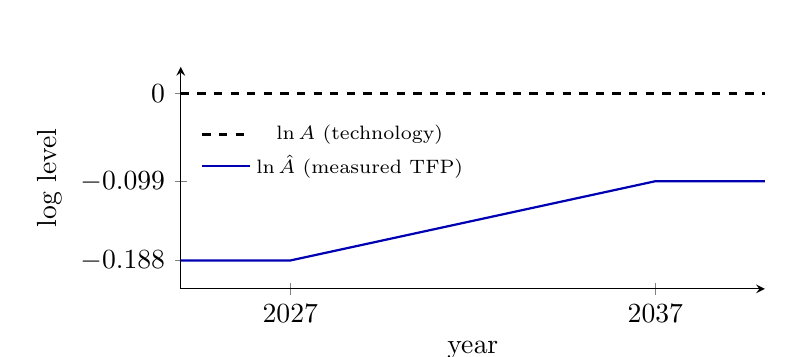
\begin{tikzpicture}
\begin{axis}[width=9cm,height=4.4cm,axis lines=left,xmin=2024,xmax=2040,ymin=-0.22,ymax=0.03,
  xlabel={year},ylabel={log level},xtick={2027,2037},xticklabels={2027,2037},
  ytick={-0.188,-0.099,0},yticklabels={$-0.188$,$-0.099$,$0$},
  legend style={font=\scriptsize,at={(0.02,0.62)},anchor=west,draw=none},
  x tick label style={/pgf/number format/1000 sep=}]
\addplot[thick,dashed,black,domain=2024:2040]{0};
\addplot[thick,blue!70!black] coordinates {(2024,-0.188) (2027,-0.188) (2037,-0.0987) (2040,-0.0987)};
\legend{$\ln A$ (technology),$\ln\hat A$ (measured TFP)}
\end{axis}
\end{tikzpicture}\\
{\footnotesize Measured TFP rises 0.89 pp a year during the reform and stops when $\theta$ stops falling; true $A$ never moves.}
\end{center}
\intuicao{The reform does not invent anything; it releases capital that was already paid for. The
data see more output from the same measured inputs and call it productivity.}
\refbib{Kurlat ch.~5, \S5.4--\S5.5 (growth accounting and what the residual contains), pp.~86--95.}
\rubrica{
\item Decomposition with the residual split into $g_{\text{TFP}}$ and the $\theta$ term: 1.5 pts.
\item $0.4\ln1.25=0.089$, about 0.89 pp per year: 1.5 pts (arithmetic slip: $-1$ pt).
\item Reverse case with the sign: 1 pt.
\item Kurlat's reading of the residual: 1 pt.
\item Residual set to zero ``because $A$ is constant'': max.\ 1 pt on the item.
}
\gap{Lista 2, 2(d), left blank: the growth-accounting residual when a capital-wasting distortion
falls. Items (a)--(c) of Lista 2 were right; this question re-asks (d) with new numbers.}
\end{sol}

% =============================================================================
\bloco{III}{Microfoundations: consumption, labour and general equilibrium}{Lectures 4--6 \,\textbullet\, 25 points}

\questao{(10 points) Objective items.}

\textbf{a)} (3 points) A two-period household (Kurlat ch.~6) has $u=\ln c_1+\beta\ln c_2$ with
$\beta=1$, faces $r=0$, can borrow and lend freely and earns $y_1=y_2=10{,}000$ reais. Consider three
separate scenarios, each against this baseline: (i) a one-off bonus of 1{,}000 today (an extraordinary
FGTS withdrawal); (ii) a credible announcement today of a raise of 1{,}000 paid in period 2 only;
(iii) a permanent raise of 1{,}000 in both periods. The changes in $c_1$ in (i), (ii), (iii) are:
\begin{alternativas}
\item 1{,}000; \ 0; \ 1{,}000
\item 500; \ 0; \ 1{,}000
\item 500; \ 500; \ 1{,}000
\item 500; \ 500; \ 500
\item 1{,}000; \ 500; \ 2{,}000
\end{alternativas}
\gabarito{C.}
\begin{sol}
With log utility $c_1=\dfrac{y_1+y_2/(1+r)}{1+\beta}=\dfrac{y_1+y_2}{2}$. (i) $\Delta W=1{,}000\Rightarrow\Delta c_1=500$;
(ii) $\Delta W=1{,}000/(1+0)=1{,}000\Rightarrow\Delta c_1=500$: news about future income moves
consumption \emph{today}, financed by borrowing; (iii) $\Delta W=2{,}000\Rightarrow\Delta c_1=1{,}000$.
\boxed{500;\ 500;\ 1{,}000}. A is Keynesian (current income only); B ignores the news.
\refbib{Kurlat ch.~6, \S6.2--\S6.3 (permanent income), pp.~105--120.}
\end{sol}

\medskip
\textbf{b)} (3 points) The government must raise a given revenue from households that save. It can tax
interest income or levy a lump-sum tax in period 2 that raises the same revenue. With CRRA utility,
which statement is correct?
\begin{alternativas}
\item Only the tax on interest changes $c_2/c_1$, through the net return in the Euler equation; at equal revenue the lump sum gives higher utility.
\item Both taxes lower $c_2/c_1$ by the same amount, because they raise the same revenue in present value and so lower wealth equally.
\item Only the lump-sum tax changes $c_2/c_1$, because it lowers wealth; the tax on interest is neutral once its revenue is fixed.
\item Only the tax on interest changes $c_2/c_1$, through the net return in the Euler equation; at equal revenue both give the same utility.
\end{alternativas}
\gabarito{A.}
\begin{sol}
Euler: $u'(c_1)=\beta[1+r(1-\tau)]u'(c_2)\Rightarrow c_2/c_1=\{\beta[1+r(1-\tau)]\}^{1/\sigma}$: the
\emph{intertemporal margin} is distorted. The lump sum shifts the budget line in parallel and leaves
$c_2/c_1=[\beta(1+r)]^{1/\sigma}$. At equal revenue $T=\tau ra$, the plan chosen under the interest tax
costs exactly $y_1+(y_2-T)/(1+r)$ at market prices, so it was affordable under the lump sum and not
chosen: \boxed{U^{\text{lump sum}}>U^{\text{interest tax}}}, the difference being deadweight loss
(D misses this).
\refbib{Kurlat ch.~6, \S6.2--\S6.4 (taxes in the two-period model), pp.~105--126.}
\end{sol}

\medskip
\textbf{c)} (2 points, T or F) A household with $u=\ln c_1+\beta\ln c_2$ earns $y_1>0$ in period 1 and
nothing in period 2 (no taxes), so it is a net saver. When $r$ rises it raises $c_1$, because for a
saver the income effect of a higher return dominates the substitution effect.
\gabarito{F.}
\begin{sol}
$c_1=\dfrac{y_1}{1+\beta}$, independent of $r$: with $\sigma=1$ and no future income to revalue, the
income and substitution effects cancel \emph{exactly}. The sign of $\partial c_1/\partial r$ is that
of $\sigma-1$; the income effect wins only if $\sigma>1$.
\refbib{Kurlat ch.~6, \S6.2 (the effect of interest rates), pp.~108--115.}
\end{sol}

\medskip
\textbf{d)} (2 points, T or F) With $u=\ln c-\chi\,h^{1+\eta}/(1+\eta)$ and no non-labour income, hours
do not respond to a permanent change in the wage (the Marshallian elasticity is zero). Therefore a
temporary, anticipated wage rise within a life of given wealth leaves hours unchanged too: the Frisch
elasticity is also zero.
\gabarito{F.}
\begin{sol}
Marshallian: $\chi h^{\eta}=w/c=w/(wh)=1/h$, hours constant. Frisch (marginal utility of wealth
$\mu$ fixed): $\chi h^{\eta}=\mu w\Rightarrow\varepsilon^F=1/\eta>0$. The ordering is
$\varepsilon^F\ge\varepsilon^H\ge\varepsilon^M$; a zero Marshallian elasticity means two effects
cancel, not that labour supply is unresponsive.
\refbib{Kurlat ch.~7, \S7.3--\S7.4, pp.~137--142.}
\gap{Lista 3, 1(b): no permanent-income story for a rise in expected $y_2$ (item a). Lista 3, 2(d): the
equal-revenue lump-sum comparison and the distorted margin were never stated (item b).}
\end{sol}

% -----------------------------------------------------------------------------
\questao{(15 points) An agribusiness productivity boom in general equilibrium.
A one-period economy has a fixed capital stock $\bar K$. The representative household owns $\bar K$ and
the firm, has one unit of time and utility $u=\dfrac{c^{1-\sigma}}{1-\sigma}+\psi\ln(1-L)$ with
$\psi=2/3$ ($\sigma$ is the curvature of utility; $1/\sigma$ the elasticity of substitution).
The competitive firm produces $Y=A\bar K^{\alpha}L^{1-\alpha}$ with $\alpha=1/3$. At the baseline
$A\bar K^{\alpha}=2^{2/3}$ and $\sigma=2$. New seed varieties raise $A$ in agriculture, which we treat
as a rise in aggregate $A$.}

\textbf{a)} (5 points) Write the household's and the firm's problems, the first-order conditions and the
market-clearing conditions. Show that profits are zero. Reduce the equilibrium to one equation in $L$,
verify that $L=1/2$ at the baseline, and compute $c$, $w$ and $r^K\bar K$.
\resolespaco
\begin{sol}
\passo{1 --- household}{$\max_{c,L}\ \frac{c^{1-\sigma}}{1-\sigma}+\psi\ln(1-L)$ s.t.\
$c=wL+r^K\bar K+\Pi$. FOC: $\boxed{\dfrac{\psi}{1-L}=w\,c^{-\sigma}}$ (MRS between leisure and
consumption $=$ real wage).}
\passo{2 --- firm}{$\max_L\ A\bar K^{\alpha}L^{1-\alpha}-wL-r^K\bar K$:
$w=(1-\alpha)\dfrac{Y}{L}$ (MPL), $r^K=\alpha\dfrac{Y}{\bar K}$ (MPK).
$\Pi=Y-(1-\alpha)Y-\alpha Y=0$ (constant returns, Euler's theorem).}
\passo{3 --- clearing}{Goods: $c=Y$ (no investment, no government). Capital: supply fixed at $\bar K$.}
\passo{4 --- one equation}{Let $\tilde A=A\bar K^{\alpha}$, so $c=\tilde AL^{1-\alpha}$ and
$w=(1-\alpha)\tilde AL^{-\alpha}$. Substituting into Step 1:
$\boxed{\psi\dfrac{L^{\alpha+(1-\alpha)\sigma}}{1-L}=(1-\alpha)\tilde A^{1-\sigma}}$ (MRS $=$ MPL).
The left side rises in $L$, so the solution is unique.}
\passo{5 --- verify}{$\sigma=2$: exponent $\tfrac13+\tfrac43=\tfrac53$. LHS at $L=\tfrac12$:
$\tfrac23\cdot\dfrac{2^{-5/3}}{2^{-1}}=\tfrac23\,2^{-2/3}$. RHS: $\tfrac23(2^{2/3})^{-1}=\tfrac23\,2^{-2/3}$ \checkmark.
Then $\boxed{c=Y=2^{2/3}\,2^{-2/3}=1}$, $\boxed{w=\tfrac23\cdot1/\tfrac12=\tfrac43}$,
$\boxed{r^K\bar K=\tfrac13}$; check $wL+r^K\bar K=\tfrac23+\tfrac13=1=Y$.}
\refbib{Kurlat ch.~9, \S9.1--\S9.2 (competitive equilibrium), pp.~165--180; ch.~7, \S7.2.}
\rubrica{
\item Both problems and FOCs, including MRS $=w$: 2 pts.
\item Zero profits and $c=Y$: 1 pt.
\item Equation in $L$ and the baseline check with $c,w,r^K\bar K$: 2 pts.
\item Adding the principal $\bar K$ to household income: $-1$ pt (budget no longer matches $c=Y$).
}
\end{sol}

\textbf{b)} (5 points) Derive $d\ln L/d\ln A$ in general and sign it by $\sigma$. Evaluate it at the
baseline and give the first-order effects of a 10\% rise in $A$ on $L$, $w$, $r^K$ and $c$. Explain in
words that match the sign.
\resolespaco
\begin{sol}
\passo{1 --- differentiate}{Log of the equation in (a):
$\ln\psi+[\alpha+(1-\alpha)\sigma]\ln L-\ln(1-L)=\ln(1-\alpha)+(1-\sigma)\ln\tilde A$.
Differentiating, with $d\ln\tilde A=d\ln A$:
$\boxed{\dfrac{d\ln L}{d\ln A}=\dfrac{1-\sigma}{\alpha+(1-\alpha)\sigma+\frac{L}{1-L}}}$.}
\passo{2 --- sign}{The denominator is positive, so the sign is that of $1-\sigma$:
$\sigma<1\Rightarrow L\uparrow$; $\sigma=1\Rightarrow L$ unchanged; $\sigma>1\Rightarrow L\downarrow$.}
\passo{3 --- baseline}{$\sigma=2$, $L=\tfrac12$: $\dfrac{-1}{\frac13+\frac43+1}=\dfrac{-1}{8/3}=\boxed{-0.375}$.}
\passo{4 --- 10\% boom}{$d\ln L=-3.75\%$. $d\ln w=d\ln A-\alpha\,d\ln L=10+\tfrac13(3.75)=\boxed{+11.25\%}$.
$d\ln r^K=d\ln A+(1-\alpha)d\ln L=10-\tfrac23(3.75)=\boxed{+7.5\%}$.
$d\ln c=d\ln Y=d\ln A+(1-\alpha)d\ln L=\boxed{+7.5\%}$.}
\passo{5 --- words}{$A\uparrow\rightarrow w\uparrow$: leisure is dearer (substitution effect, work more)
but the household is richer (income effect, enjoy more leisure). With $\sigma=2$ marginal utility of
consumption falls fast as $c$ rises, so the \emph{income effect dominates} and hours fall. Output and
consumption still rise, by less than $A$.}
\intuicao{$\sigma$ measures how fast extra consumption loses value. Above one, a richer household
prefers to take part of its gain as leisure; at exactly one the two effects cancel.}
\refbib{Kurlat ch.~7, \S7.2 (income and substitution effects), pp.~131--137; ch.~9, \S9.2.}
\rubrica{
\item Correct derivative: 2 pts. Sign by $\sigma$ with the three cases: 1 pt.
\item $-0.375$ and the four effects: 1 pt (arithmetic slip: $-1$ pt, non-cumulative).
\item Words matching the sign: 1 pt.
\item Words describing only the substitution effect (``higher wage, so they work more'') when the derivative is negative: max.\ 3 pts on the item.
}
\end{sol}

\textbf{c)} (5 points) Now set $\sigma=1$. The government taxes labour income at $\tau=0.25$.
Compute equilibrium hours without the tax and in two cases: (i) the revenue is rebated lump sum;
(ii) the revenue is thrown away (spent on something with no value to the household). Explain why hours
fall in (i) even with log utility, why they fall less in (ii), and what happens in (ii) if $\alpha\to0$.
\resolespaco
\begin{sol}
\passo{1 --- FOC with the tax}{Budget $c=(1-\tau)wL+r^K\bar K+T$; FOC
$\dfrac{\psi}{1-L}=\dfrac{(1-\tau)w}{c}$, with $w=(1-\alpha)Y/L$.}
\passo{2 --- no tax}{$c=Y$: $\psi\dfrac{L}{1-L}=1-\alpha\Rightarrow\tfrac23\dfrac{L}{1-L}=\tfrac23\Rightarrow\boxed{L=\tfrac12}$.}
\passo{3 --- (i) rebate}{$T=\tau wL\Rightarrow c=Y$:
$\psi\dfrac{L}{1-L}=(1-\tau)(1-\alpha)=0.75\cdot\tfrac23=0.5\Rightarrow
L=\dfrac{0.5}{\frac23+0.5}=\boxed{\tfrac37\approx0.429}$.}
\passo{4 --- (ii) thrown away}{$c=Y-\tau wL=Y[1-\tau(1-\alpha)]$:
$\psi\dfrac{L}{1-L}=\dfrac{(1-\tau)(1-\alpha)}{1-\tau(1-\alpha)}=\dfrac{0.5}{5/6}=0.6\Rightarrow
\dfrac{L}{1-L}=0.9\Rightarrow\boxed{L=\tfrac{9}{19}\approx0.474}$.}
\passo{5 --- why (i) falls}{The rebate hands back the revenue: total income is unchanged ($c=Y$) but the
price of leisure falls to $(1-\tau)w$. The transfer is non-labour income that does not shrink with
the net wage, so the tax acts as a \emph{compensated} wage cut: a pure substitution effect $\Rightarrow$
hours fall, with log utility or not.}
\passo{6 --- why (ii) falls less, and $\alpha\to0$}{Without the rebate the household is poorer. On
labour income, log utility makes the income and substitution effects cancel; only the capital rents
$r^K\bar K$ (share $\alpha$), unearned income that does not fall with the net wage, leave a residual
effect. As $\alpha\to0$ the right side tends to $(1-\tau)/(1-\tau)=1$ and
\boxed{L\text{ is independent of }\tau}.}
\intuicao{With log consumption utility, a wage tax changes hours only through non-labour income ---
the transfer and the capital rents. Set that income to zero and the effect vanishes; the story must
therefore be about the transfer.}
\refbib{Kurlat ch.~7, \S7.2 (taxes and labour supply), pp.~131--137; ch.~9, \S9.2.}
\rubrica{
\item FOC with $(1-\tau)w$: 1 pt. $L=\tfrac12$, $\tfrac37$, $\tfrac{9}{19}$: 2 pts (slip: $-1$ pt).
\item Rebate $=$ compensated change, substitution effect only: 1 pt.
\item Role of non-labour income in (ii) and the $\alpha\to0$ limit: 1 pt.
\item Explaining (i) by ``the tax lowers the wage, so leisure is cheaper'' with no role for the transfer, and claiming the same in (ii): max.\ 2 pts on the item.
}
\gap{Lista 4, 1(b): with log utility labour responds to a wage tax only through the transfer, but the
words described the substitution effect. Lista 5, Q1: the sign of $d\ln L/d\ln A$ is that of
$1-\sigma$ and the words must match it.}
\end{sol}

% =============================================================================
\bloco{IV}{Money, inflation and the New-Keynesian AS--AD model}{Lectures 7--9 \,\textbullet\, 25 points}

\questao{(10 points) Objective items.}

\textbf{a)} (3 points) A flexible-price economy (Kurlat ch.~11) has real money demand $M/P=Y\,\ell(i)$,
$\ell'<0$, with $Y$ and $r$ fixed by the real side. Which statement is correct?
\begin{alternativas}
\item A one-off 10\% rise in $M$ raises $P$ by 10\% and leaves $Y$, $r$ and $M/P$ unchanged; a permanent rise in money growth also leaves $M/P$ unchanged, as money is superneutral.
\item A one-off 10\% rise in $M$ raises $P$ by 10\% and leaves $Y$, $r$ and $M/P$ unchanged; a permanent rise in money growth raises $i$ and lowers $M/P$.
\item A one-off 10\% rise in $M$ lowers $i$ through a liquidity effect and raises $Y$ for good; a permanent rise in money growth raises $i$ and lowers $M/P$.
\item A one-off 10\% rise in $M$ raises $P$ by 10\% and leaves $Y$, $r$ and $M/P$ unchanged; under a Selic target the Copom fixes both $i$ and $M$ independently.
\end{alternativas}
\gabarito{B.}
\begin{sol}
Level change: neutrality, $P$ moves one for one. Growth change: $\pi\uparrow\Rightarrow i=r+\pi\uparrow
\Rightarrow\ell(i)\downarrow$: money is neutral but \emph{not superneutral} (A). C is IS--LM with
flexible prices. D: with $i$ as the instrument, $M=P\,Y\ell(\bar\imath)$ is \emph{determined} by the
money market; the bank cannot also choose $M$.
\refbib{Kurlat ch.~11, \S11.1--\S11.2, pp.~205--215; ch.~10 on the instrument.}
\end{sol}

\medskip
\textbf{b)} (3 points) Real money demand is $M/P=0.10\,Y\,e^{-4\pi}$ (Cagan form, $\pi$ in decimal per
year), $Y$ is constant and in steady state $\pi$ equals money growth. The inflation rate that maximises
seigniorage, and seigniorage at that rate, are:
\begin{alternativas}
\item $\pi=12.5\%$; seigniorage $0.76\%$ of GDP
\item $\pi=25\%$; seigniorage $2.50\%$ of GDP
\item $\pi=50\%$; seigniorage $0.68\%$ of GDP
\item $\pi=25\%$; seigniorage $0.92\%$ of GDP
\end{alternativas}
\gabarito{D.}
\begin{sol}
$S/Y=\pi\cdot0.10e^{-4\pi}$; $\frac{d}{d\pi}=0.10e^{-4\pi}(1-4\pi)=0\Rightarrow\boxed{\pi=1/a=25\%}$;
$S/Y=0.25\cdot0.10\cdot e^{-1}=\boxed{0.92\%}$. B ignores the erosion of the base ($0.25\times0.10$);
A and C are off the peak ($0.76\%$, $0.68\%$).
\refbib{Kurlat ch.~11, \S11.3 (seigniorage) and Exercise 11.6 (Cagan), pp.~215--222.}
\end{sol}

\medskip
\textbf{c)} (2 points, T or F) In Benigno's AS--AD model, a cut in the Selic moves the economy along the
AS curve.
\gabarito{T.}
\begin{sol}
$i$ enters only AD. The cut shifts AD up and to the right; AS (anchored at $(p^e,y_n)$) does not move,
so the new equilibrium lies further up the same AS: $y\uparrow$, $p\uparrow$.
\refbib{Benigno (2015), \S5, Figs.~3--5, pp.~509--511.}
\end{sol}

\medskip
\textbf{d)} (2 points, T or F) In Benigno's model, natural output $y_n$ differs from efficient output
$y_e$ because a fraction of prices is sticky.
\gabarito{F.}
\begin{sol}
$y_n$ is the flexible-price equilibrium, $y_e$ the planner's choice; the stickiness share $\alpha$ is
in neither. The gap is the mark-up wedge (market power and taxes): $y_n-y_e=-\mu/(\sigma^{-1}+\eta)$.
Stickiness explains $y\neq y_n$.
\refbib{Benigno (2015), \S4.2--\S4.4, eqs.~(15), (19), pp.~508--509.}
\gap{Lista 6, 1(c)--(d): flexible prices $\Rightarrow$ neutrality; under an interest-rate instrument
the money market determines $M$ (item a). Lista 7 traps 1 and 4 (items c, d).}
\end{sol}

% -----------------------------------------------------------------------------
\questao{(15 points) A mark-up shock in fuel distribution.
A merger wave concentrates fuel distribution and raises firms' desired mark-up by 4.4\% for one period
only. Use Benigno's model in log deviations from an efficient steady state, with no public spending
($g=0$), no tax changes, $\bar p=p^e=0$ and $\bar y_n=0$:
\[
\text{AS: } p-p^e=\kappa(y-y_n),\quad \kappa=\frac{(1-\alpha)(\sigma^{-1}+\eta)}{\alpha};\qquad
\text{AD: } y=\bar y_n-\sigma\left[i-(\bar p-p)-\rho\right].
\]
Calibration: $\alpha=0.66$ (share of sticky prices), $\sigma=0.5$, $\eta=0.2$, $\theta=8$, $\rho=5\%$.
Before the shock $i=\rho$, $y=y_n=y_e=0$ and $p=p^e$. At first the Copom keeps the Selic at 5\%.}

\textbf{a)} (5 points) Which curve shifts and which does not, and why? Find $y$ and $p$, and the signs
of $y-y_n$ and $y-y_e$. Draw the AS--AD diagram and the time path of $y$ and $p$ over the short run
(period 1) and the long run (period 2).
\resolespaco
\begin{sol}
\passo{1 --- slope}{$\kappa=\dfrac{0.34\cdot(2+0.2)}{0.66}=\dfrac{0.748}{0.66}=1.133$; $\sigma\kappa=0.567$.}
\passo{2 --- what shifts}{$y_n=\dfrac{(1+\eta)a-\mu}{\sigma^{-1}+\eta}\Rightarrow dy_n=-\dfrac{4.4}{2.2}=\boxed{-2\%}$;
$y_e$ has no $\mu$, $dy_e=0$. \boxed{\text{AS shifts up/left}} through $(p^e,y_n'=-2)$, by
$\kappa\cdot2=2.27$ pp at given $y$ ($=\frac{1-\alpha}{\alpha}d\mu=0.515\cdot4.4$ \checkmark).
\boxed{\text{AD does not shift}}: $\mu$ is not in AD, $i$ is unchanged, and a \emph{temporary} shock leaves $\bar y_n$ unchanged.}
\passo{3 --- equilibrium}{AD with $i=\rho$: $p=-y/\sigma=-2y$. AS: $p=1.133(y+2)$.
$-2y=1.133y+2.267\Rightarrow y=-\dfrac{2.267}{3.133}=\boxed{-0.72\%}$, $\boxed{p=+1.45\%}$: stagflation.
(Closed form: $dy=\frac{\sigma\kappa}{1+\sigma\kappa}dy_n$, $dp=-\frac{\kappa}{1+\sigma\kappa}dy_n$.)}
\passo{4 --- two gaps}{$\boxed{y-y_n=-0.72+2=+1.28>0}$ (why prices rise: AS responds to $y-y_n$);
$\boxed{y-y_e=-0.72<0}$ (why welfare falls).}
\passo{5 --- chain}{$\mu\uparrow\rightarrow$ adjusting firms raise prices $\rightarrow p\uparrow
\rightarrow$ real rate $i-(\bar p-p)\uparrow\rightarrow c\downarrow\rightarrow y\downarrow$ along AD.
LR: the shock is over, all firms reset, $y=\bar y_n=0$, $p=\bar p=0$.}
\begin{center}
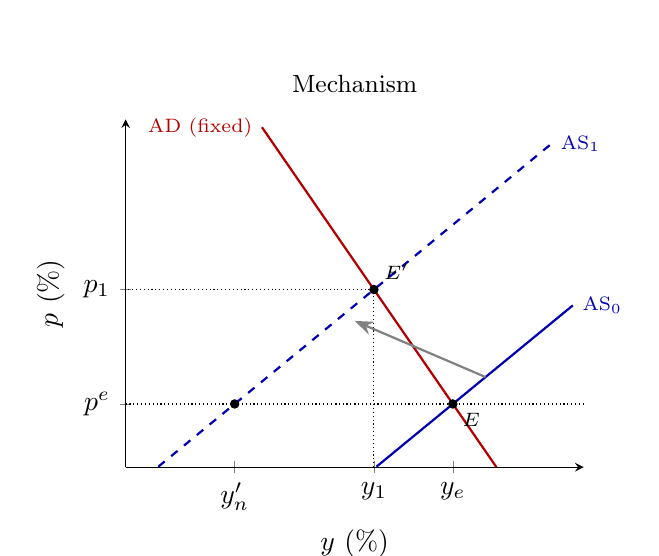
\begin{tikzpicture}
\begin{axis}[width=7.4cm,height=6cm,axis lines=left,xmin=-3,xmax=1.2,ymin=-0.8,ymax=3.6,clip=false,
  xlabel={$y$ (\%)},ylabel={$p$ (\%)},xtick={-2,-0.7234,0},xticklabels={$y_n'$,$y_1$,$y_e$},
  ytick={0,1.4468},yticklabels={$p^e$,$p_1$},title={\small Mechanism}]
\addplot[densely dotted,domain=-3:1.2]{0};
\addplot[thick,blue!70!black,domain=-0.7:1.1]{1.1333*x};
\addplot[thick,blue!70!black,dashed,domain=-2.7:0.9]{1.1333*(x+2)};
\addplot[thick,red!70!black,domain=-1.75:0.4]{-2*x};
\node[font=\scriptsize,blue!70!black,anchor=west] at (axis cs:1.1,1.25) {AS$_0$};
\node[font=\scriptsize,blue!70!black,anchor=west] at (axis cs:0.9,3.29) {AS$_1$};
\node[font=\scriptsize,red!70!black,anchor=east] at (axis cs:-1.75,3.5) {AD (fixed)};
\addplot[only marks,mark=*,mark size=1.5pt] coordinates {(0,0) (-0.7234,1.4468) (-2,0)};
\node[font=\scriptsize,anchor=north west] at (axis cs:0,0) {$E$};
\node[font=\scriptsize,anchor=south west] at (axis cs:-0.72,1.45) {$E'$};
\draw[densely dotted] (axis cs:-0.7234,-0.8)--(axis cs:-0.7234,1.4468)--(axis cs:-3,1.4468);
\draw[-{Stealth},thick,gray] (axis cs:0.3,0.34)--(axis cs:-0.9,1.05);
\end{axis}
\end{tikzpicture}\quad
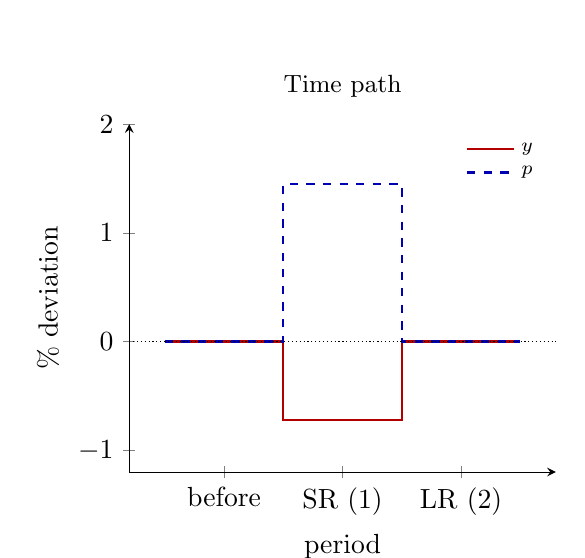
\begin{tikzpicture}
\begin{axis}[width=7cm,height=6cm,axis lines=left,xmin=-0.3,xmax=3.3,ymin=-1.2,ymax=2,
  xlabel={period},xtick={0.5,1.5,2.5},xticklabels={before,SR (1),LR (2)},ylabel={\% deviation},
  title={\small Time path},legend style={font=\scriptsize,draw=none,at={(0.98,0.98)},anchor=north east}]
\addplot[thick,red!70!black,const plot] coordinates {(0,0) (1,-0.7234) (2,0) (3,0)};
\addplot[thick,blue!70!black,dashed,const plot] coordinates {(0,0) (1,1.4468) (2,0) (3,0)};
\addplot[densely dotted,domain=-0.3:3.3]{0};
\legend{$y$,$p$}
\end{axis}
\end{tikzpicture}
\end{center}
\intuicao{The mark-up raises prices at any output; with $\bar p$ anchored, a higher $p$ is a higher real
rate, so demand falls along AD. Output does not fall all the way to $y_n'$ because the sticky firms keep
selling at $p^e$.}
\refbib{Benigno (2015), \S7, Fig.~9, pp.~513--514; \S5, eqs.~(20)--(21).}
\rubrica{
\item AS shifts up/left and AD explicitly does \emph{not} move, with reasons: 1.5 pts.
\item $y=-0.72$, $p=+1.45$: 1 pt (slip: $-1$ pt).
\item Both gaps with opposite signs: 1 pt.
\item Diagram: axes, AS$_0$, AS$_1$ and the unmoved AD labelled, direction of shift: 1 pt; time path SR/LR: 0.5 pt.
\item Shifting AD: max.\ 2 pts on the item. Reporting a single ``output gap'': max.\ 3.5 pts.
}
\end{sol}

\textbf{b)} (5 points) With $u(C)=\dfrac{C^{1-1/\sigma}}{1-1/\sigma}$, $v(L)=\dfrac{L^{1+\eta}}{1+\eta}$,
$Y=AL$ and $C=Y$, the market's labour-supply condition is $\text{MRS}=A/(1+\mu)$ and the planner's is
$\text{MRS}=A$. Derive both, log-linearise, and show $y_n-y_e=-\mu/(\sigma^{-1}+\eta)$. Explain why sticky
prices play no role, and evaluate the gap for this shock.
\resolespaco
\begin{sol}
\passo{1 --- planner}{$\max_Y u(Y)-v(Y/A)$: $u'(Y)=v'(L)/A\Rightarrow\boxed{\dfrac{v'(L)}{u'(C)}=A}$
(MRS $=$ MRT).}
\passo{2 --- market}{Flexible-price firms set $P=(1+\mu)W/A\Rightarrow W/P=A/(1+\mu)$; the household sets
MRS $=W/P$: $\boxed{\dfrac{v'(L)}{u'(C)}=\dfrac{A}{1+\mu}}$. Same condition up to the wedge $1+\mu$.}
\passo{3 --- logs}{$\ln v'=\eta l=\eta(y-a)$; $\ln u'=-\sigma^{-1}c=-\sigma^{-1}y$. So
$\ln\text{MRS}=\eta(y-a)+\sigma^{-1}y$. Planner: $=a\Rightarrow y_e=\dfrac{(1+\eta)a}{\sigma^{-1}+\eta}$.
Market: $=a-\mu\Rightarrow y_n=\dfrac{(1+\eta)a-\mu}{\sigma^{-1}+\eta}$.}
\passo{4 --- subtract}{$\boxed{y_n-y_e=-\dfrac{\mu}{\sigma^{-1}+\eta}}=-\dfrac{4.4}{2.2}=\boxed{-2\%}$.}
\passo{5 --- no stickiness}{$\alpha$ appears in neither condition: $y_n$ is the equilibrium when
\emph{all} prices are flexible; $y_e$ is the planner's, with no prices at all. \#~Stickiness explains
$y\neq y_n$ (it sits in $\kappa$); market power and taxes explain $y_n\neq y_e$. A productivity shock
moves both by $(1+\eta)/(\sigma^{-1}+\eta)$: efficient, no gap.}
\intuicao{A firm with market power pays labour $A/(1+\mu)$ of what it produces; households work until
their MRS equals what they are paid, not what they produce, so the market works and produces too little.}
\refbib{Benigno (2015), \S4.1--\S4.4, eqs.~(14), (15), (19), pp.~507--509.}
\rubrica{
\item Planner MRS $=A$ and market MRS $=A/(1+\mu)$ derived: 2 pts.
\item Log-linearisation and the boxed gap: 1.5 pts; $-2\%$: 0.5 pt.
\item Why stickiness plays no role: 1 pt.
\item Attributing $y_n\neq y_e$ to sticky prices: max.\ 2 pts on the item.
}
\end{sol}

\textbf{c)} (5 points) The Copom minimises $\mathcal L=\phi_y(y-y_e)^2+\phi_p(p-p^e)^2$ with Benigno's
welfare weights $\phi_y=\tfrac12$, $\phi_p=\theta/(2\kappa)$, subject to AS. Derive the targeting rule by
substitution, the optimal $y$ and $p$ and the split of the shock, and the Selic that implements it.
Explain why AS and not AD is the constraint, and what the money market does. Is the optimal response a
rise or a cut relative to doing nothing, and on what does that sign depend?
\resolespaco
\begin{sol}
\passo{1 --- substitute AS}{$\mathcal L(y)=\phi_y y^2+\phi_p\kappa^2(y-y_n)^2$ (with $y_e=0$).
FOC: $\phi_y y+\phi_p\kappa^2(y-y_n)=0$; using $\kappa(y-y_n)=p-p^e$:
$\boxed{\phi_y(y-y_e)+\kappa\phi_p(p-p^e)=0}$; with the welfare weights, $(y-y_e)+\theta(p-p^e)=0$.}
\passo{2 --- optimum}{$\phi_p\kappa^2/\phi_y=\theta\kappa=8\cdot1.133=9.067$.
$y^o=\dfrac{\theta\kappa}{1+\theta\kappa}y_n=0.901\cdot(-2)=\boxed{-1.80\%}$;
$y^o-y_n=\dfrac{2}{1+\theta\kappa}=0.199$; $p^o-p^e=\kappa\cdot0.199=\boxed{+0.23\%}$.
Split: $1/(1+\theta\kappa)=9.9\%$ of the distance $y_e-y_n$ is accepted as output above $y_n$ (hence
prices); $90.1\%$ is absorbed as an output loss. Check: $-1.80+8(0.225)=0$ \checkmark.}
\passo{3 --- the Selic}{Combining AS and AD: $y-y_n=\dfrac{\sigma}{1+\sigma\kappa}(r_n-i)$, with
$r_n=\rho+\sigma^{-1}(\bar y_n-y_n)=5+2\cdot2=9\%$. So
$i^o=9-\dfrac{1.567}{0.5}(0.199)=9-0.623=\boxed{8.38\%}$. Check on AD: $p=5-8.38+2(1.80)=0.23$ \checkmark.
Strict price stability needs $i=r_n=9\%$; strict output stabilisation $i=9-3.133\cdot2=2.73\%$.
Loss: 1.80 at the optimum vs 7.65 with $i=5\%$.}
\passo{4 --- why AS}{One instrument, $i$, which appears only in AD. For any point on AS there is an $i$
that puts AD through it, so AD restricts nothing: it is how the choice is \emph{implemented}. AS is
private pricing behaviour with $p^e$ predetermined, which policy cannot move within the period: it is
the feasible set, like a budget line. The money market has no role in the choice: with $i$ fixed, the
central bank supplies whatever $M=P\,\ell(Y,i)$ is demanded, so it only determines $M$ --- which is why
the model has no LM curve.}
\passo{5 --- sign}{With $i=5\%$, $y-y_n=\dfrac{y_e-y_n}{1+\sigma\kappa}=1.28$; optimum
$\dfrac{y_e-y_n}{1+\theta\kappa}=0.20$. Lower $y-y_n$ needs a higher rate:
\boxed{\text{a rise of }3.38\text{ pp}}. It is a rise iff $\theta\kappa>\sigma\kappa\iff\theta>\sigma$
(general weights: $(\phi_p/\phi_y)\kappa>\sigma$), i.e.\ iff the IT line (slope $-1/\theta$) is flatter
than AD (slope $-1/\sigma$). A dovish bank with $(\phi_p/\phi_y)\kappa<\sigma$ would \emph{cut}.}
\begin{center}
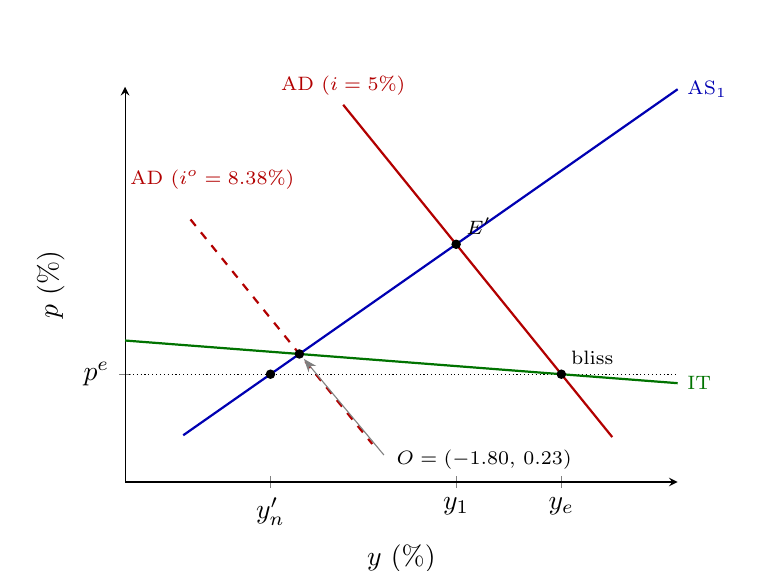
\begin{tikzpicture}
\begin{axis}[width=8.6cm,height=6.6cm,axis lines=left,xmin=-3,xmax=0.8,ymin=-1.2,ymax=3.2,clip=false,
  xlabel={$y$ (\%)},ylabel={$p$ (\%)},xtick={-2,-0.7234,0},xticklabels={$y_n'$,$y_1$,$y_e$},
  ytick={0},yticklabels={$p^e$}]
\addplot[densely dotted,domain=-3:0.8]{0};
\addplot[thick,blue!70!black,domain=-2.6:0.8]{1.1333*(x+2)};
\addplot[thick,green!45!black,domain=-3:0.8]{-x/8};
\addplot[thick,red!70!black,domain=-1.5:0.35]{-2*x};
\addplot[thick,red!70!black,dashed,domain=-2.55:-1.3]{-3.377-2*x};
\node[font=\scriptsize,blue!70!black,anchor=west] at (axis cs:0.8,3.17) {AS$_1$};
\node[font=\scriptsize,green!45!black,anchor=west] at (axis cs:0.8,-0.1) {IT};
\node[font=\scriptsize,red!70!black,anchor=south] at (axis cs:-1.5,3.0) {AD ($i=5\%$)};
\node[font=\scriptsize,red!70!black,anchor=south] at (axis cs:-2.4,1.95) {AD ($i^o=8.38\%$)};
\addplot[only marks,mark=*,mark size=1.5pt] coordinates {(-0.7234,1.4468) (-1.8013,0.2252) (0,0) (-2,0)};
\node[font=\scriptsize,anchor=south west] at (axis cs:-0.72,1.45) {$E'$};
\node[font=\scriptsize,anchor=west] at (axis cs:-1.2,-0.95) {$O=(-1.80,\,0.23)$};
\draw[-{Stealth},gray] (axis cs:-1.22,-0.9)--(axis cs:-1.77,0.17);
\node[font=\scriptsize,anchor=south west] at (axis cs:0,0) {bliss};
\end{axis}
\end{tikzpicture}\\
{\footnotesize The optimum $O$ is where AS$_1$ meets the IT line $(y-y_e)+\theta(p-p^e)=0$; the Copom raises $i$ so that AD shifts
down/left from $E'$ to $O$. AS does not move with policy.}
\end{center}
\intuicao{A mark-up shock moves $y_n$ but not $y_e$, so no rate delivers both targets. Convex losses
make the bank spread the miss; with welfare weights, relative-price dispersion is so costly
($\theta=8$) that it lets only a tenth of the shock into prices.}
\refbib{Benigno (2015), \S11, eqs.~(33)--(35), Fig.~14, pp.~521--523; \S3 on the interest-rate instrument.}
\rubrica{
\item Targeting rule by substitution: 1.5 pts.
\item $y^o=-1.80$, $p^o=+0.23$, split $1/(1+\theta\kappa)$: 1 pt (slip: $-1$ pt).
\item $i^o=8.38\%$ via $r_n=9\%$: 0.5 pt.
\item Why AS is the constraint and the money market determines $M$: 1 pt.
\item Sign relative to no policy with the condition $\theta>\sigma$: 1 pt.
\item Using AD as the constraint: max.\ 2 pts on the item. Targeting $y_n$ instead of $y_e$: max.\ 2.5 pts.
}
\gap{Lista 7 (latest content): a temporary mark-up shock moves only AS; $y-y_n$ vs $y-y_e$; why
$y_n\neq y_e$ (wedge, not stickiness); optimal policy subject to AS and why AD is not a constraint.
Lista 6, 1(d): under a rate instrument the money market determines $M$.}
\end{sol}

\ifsolucoes\else
\vfill
\begin{center}\footnotesize\textit{End of exam.}\end{center}
\fi

\end{document}
